%%%%%%%%%%%%%%%%%%%%%%%%%%%%%%%%%%%%%%%%%%%%%%%%%%%%%%%%%%%%%%%%%%%%%%%%%%%%%%%%%%
\begin{frame}[fragile]\frametitle{}
\begin{center}
{\Large What is Graph Data Science}

{\tiny (Primarily based on deck by Alison Cossette - neo4j)}
\end{center}
\end{frame}

%%%%%%%%%%%%%%%%%%%%%%%%%%%%%%%%%%%%%%%%%%%%%%%%%%%%%%%%%%%%%%%%%%%%%%%%%%%%%%%%%%
\begin{frame}[fragile]\frametitle{Everything is Naturally Connected}

\begin{center}
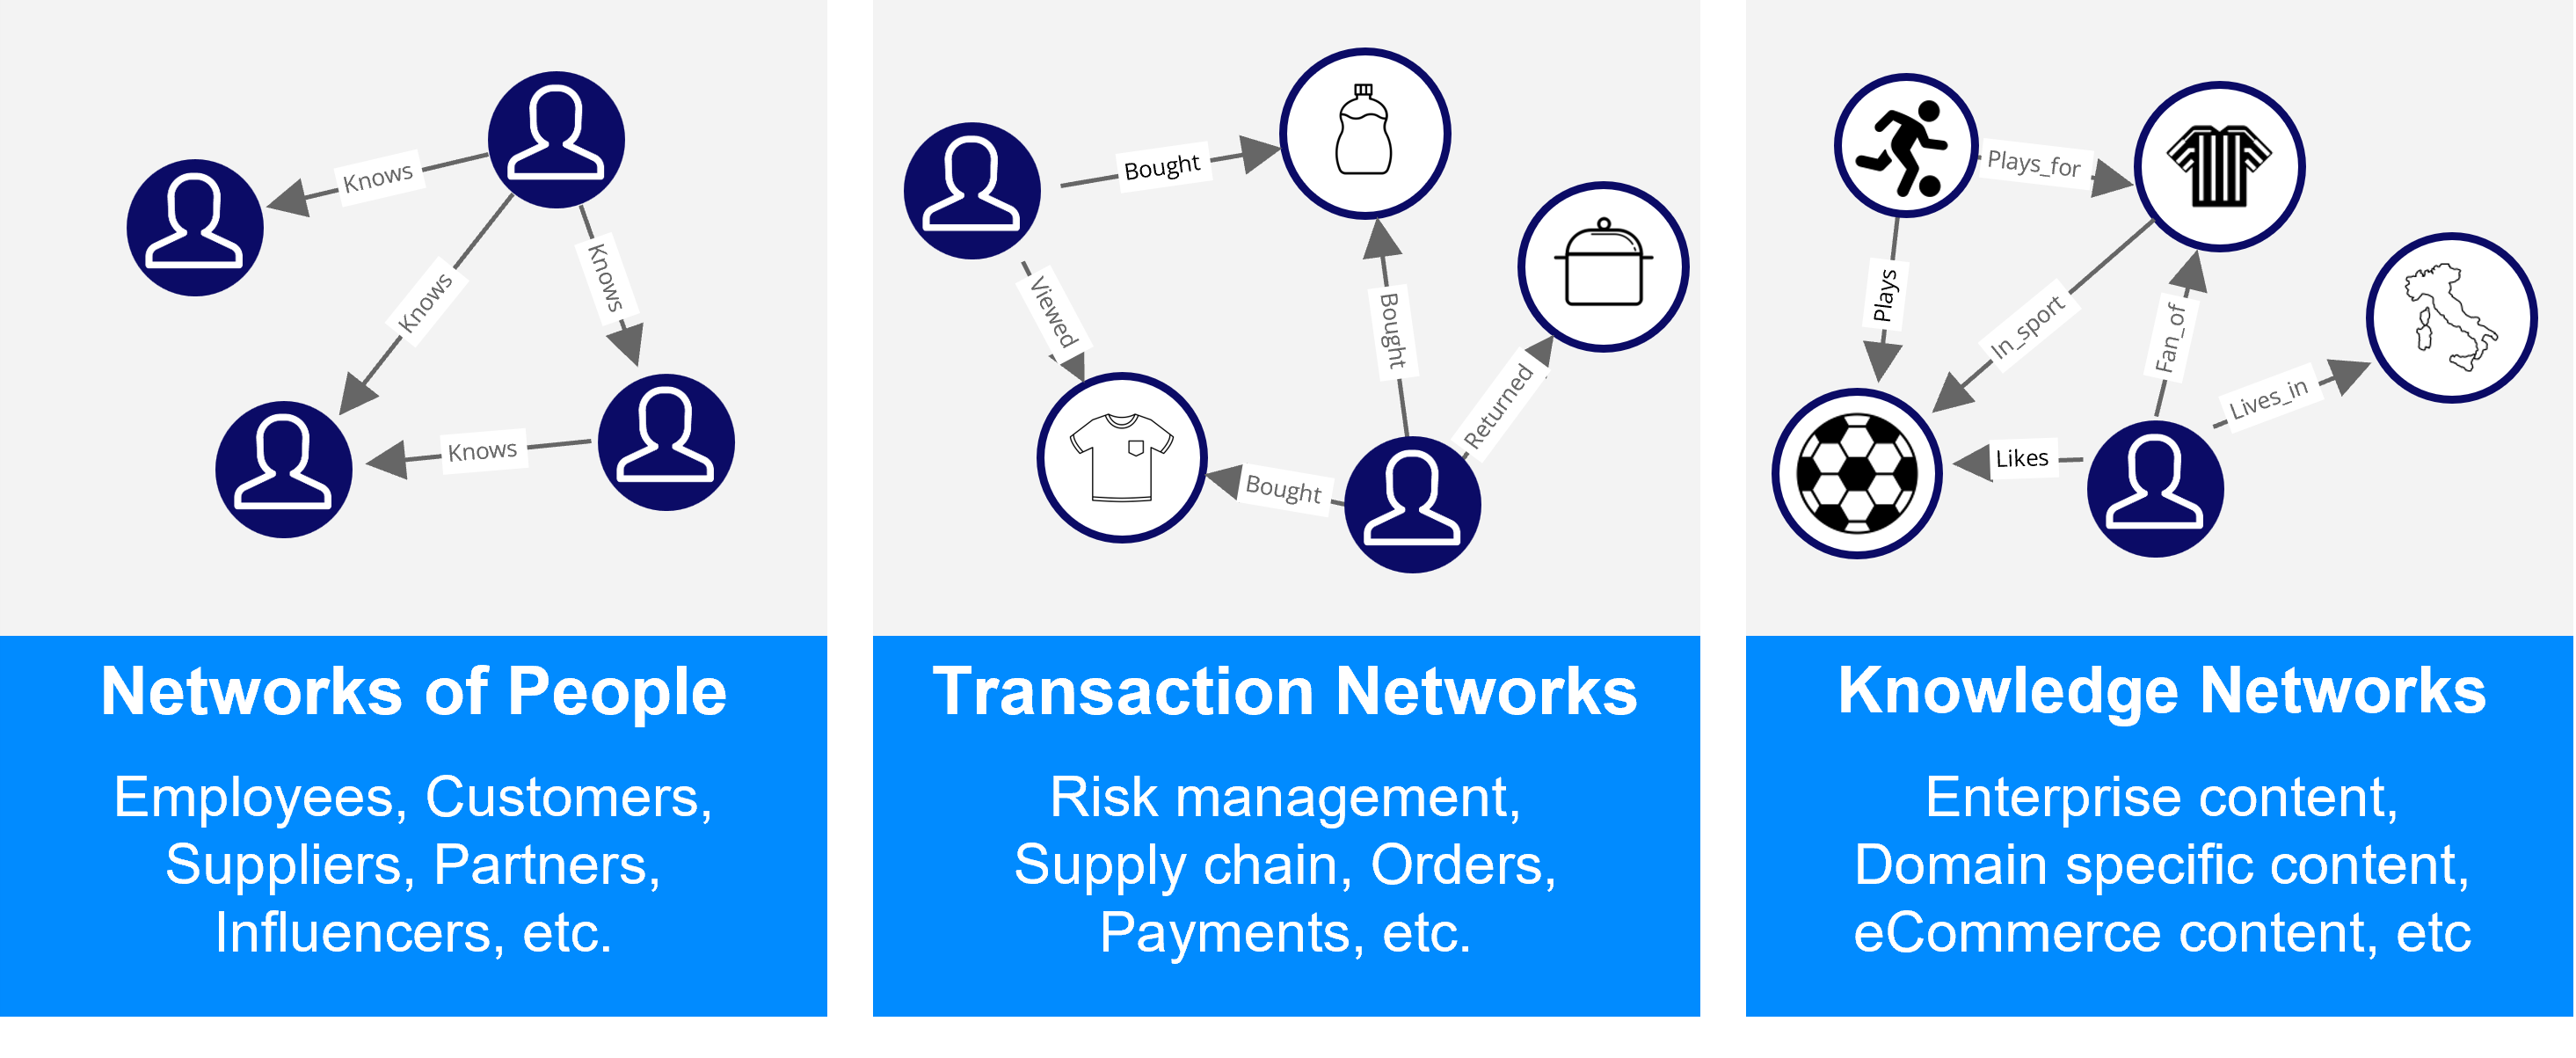
\includegraphics[width=\linewidth,keepaspectratio]{gds1}
\end{center}

\end{frame}

%%%%%%%%%%%%%%%%%%%%%%%%%%%%%%%%%%%%%%%%%%%%%%%%%%%%%%%%%%%%%%%%%%%%%%%%%%%%%%%%%%
\begin{frame}[fragile]\frametitle{Example}

\begin{center}
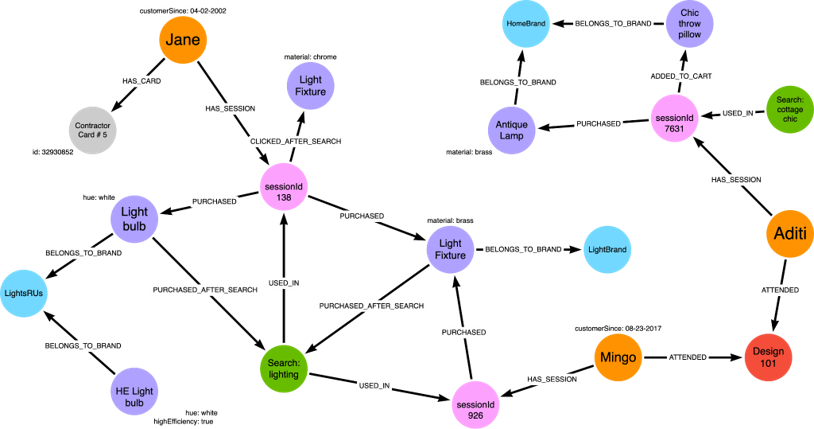
\includegraphics[width=\linewidth,keepaspectratio]{gds2}
\end{center}

\end{frame}

%%%%%%%%%%%%%%%%%%%%%%%%%%%%%%%%%%%%%%%%%%%%%%%%%%%%%%%%%%%%%%%%%%%%%%%%%%%%%%%%%%
\begin{frame}[fragile]\frametitle{Can you imagine?}

Graph to Tabular data for ML \ldots

\begin{center}
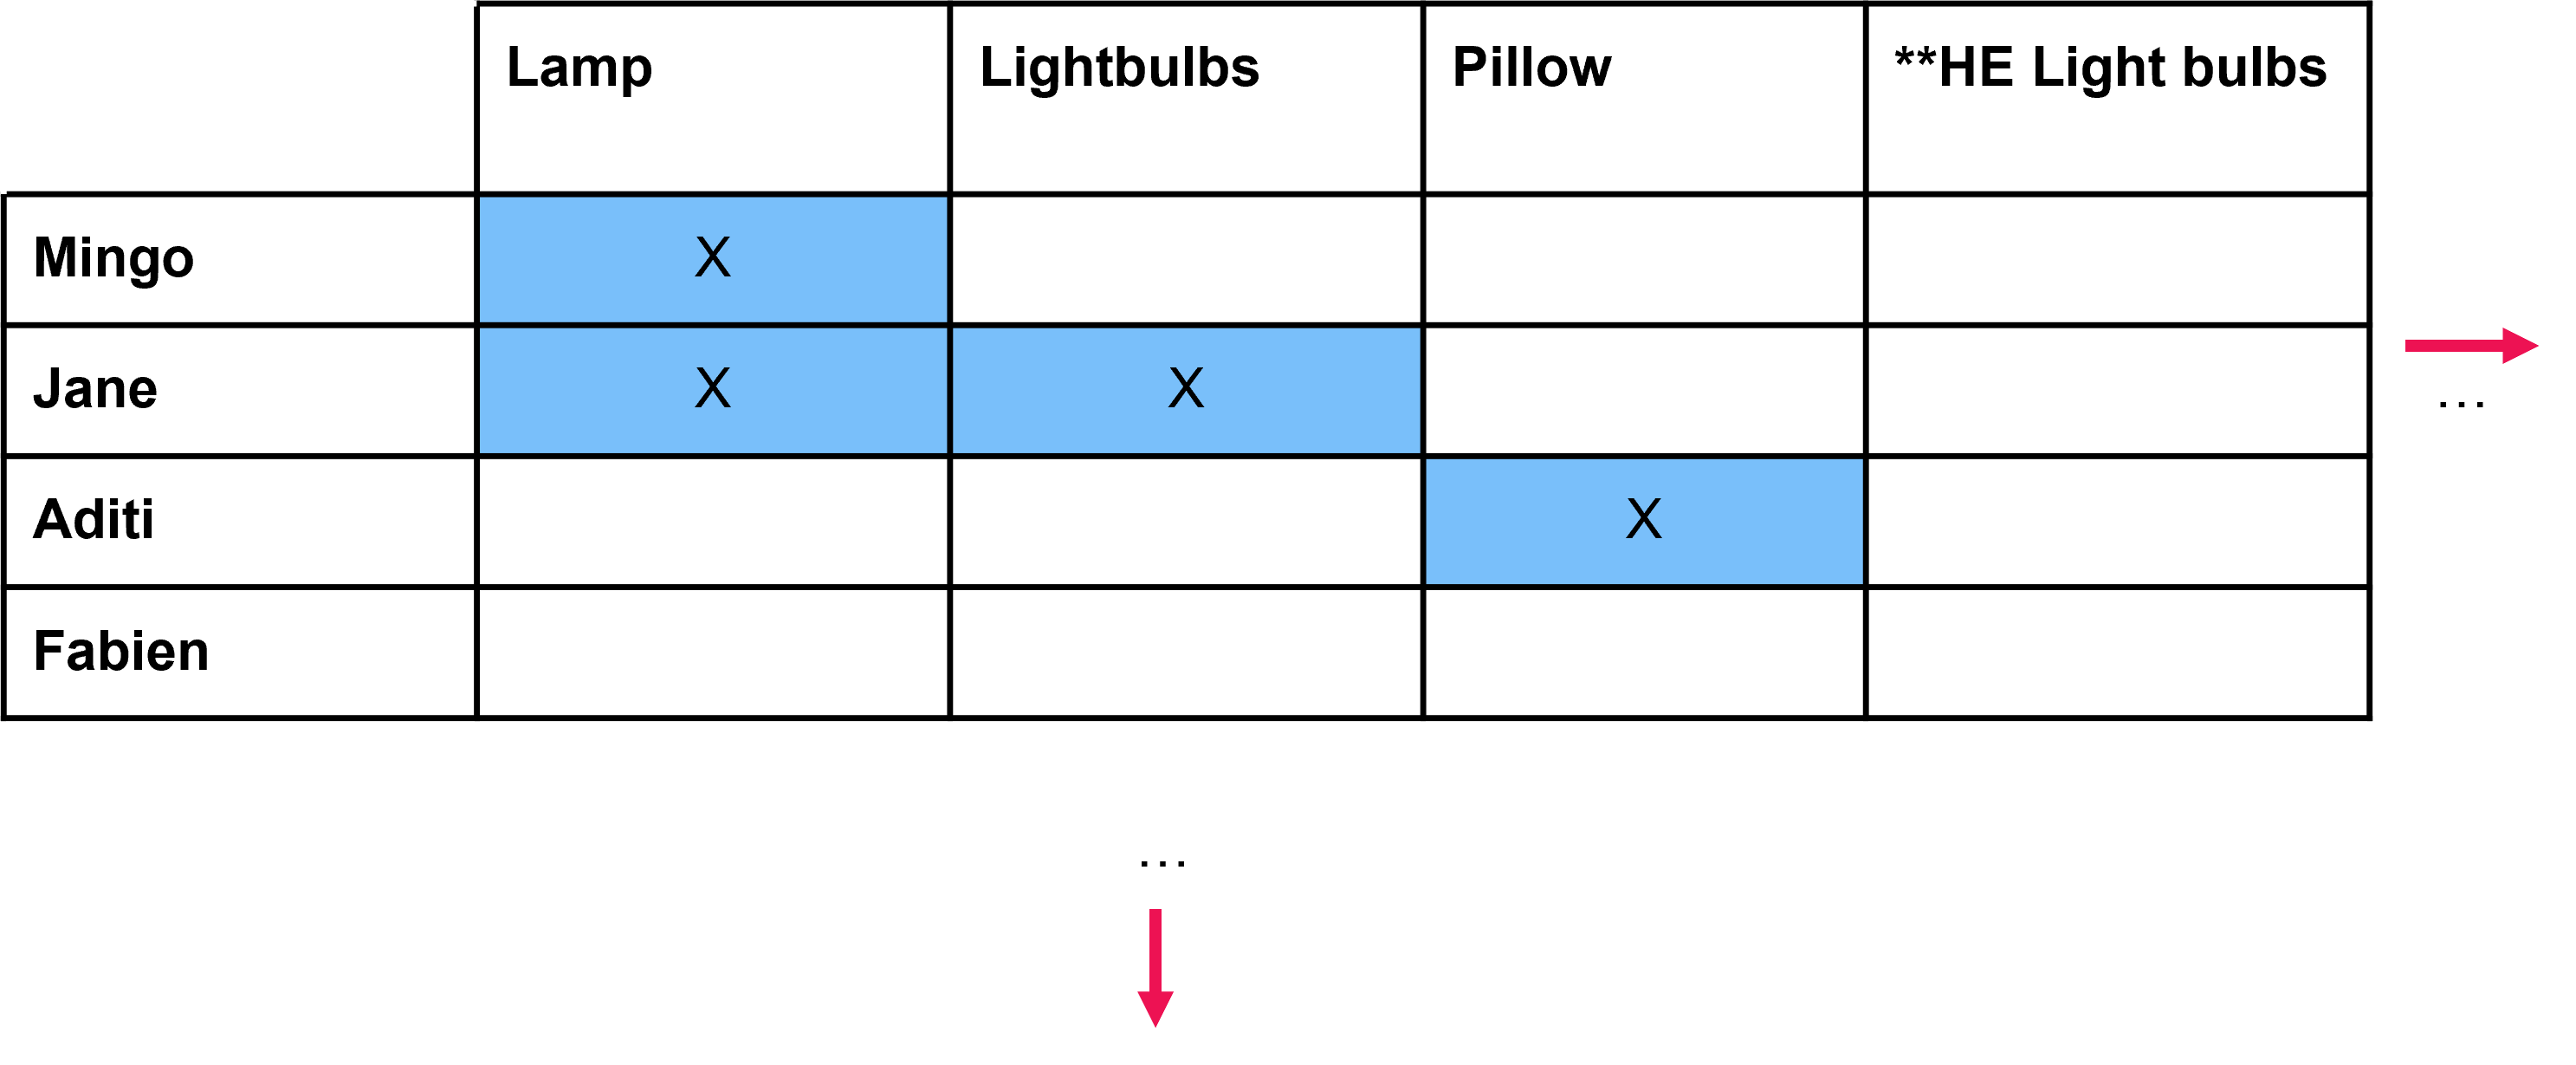
\includegraphics[width=\linewidth,keepaspectratio]{gds3}
\end{center}

\end{frame}


%%%%%%%%%%%%%%%%%%%%%%%%%%%%%%%%%%%%%%%%%%%%%%%%%%%%%%%%%%%%%%%%%%%%%%%%%%%%%%%%%%
\begin{frame}[fragile]\frametitle{What's the problem?}

\begin{itemize}
\item History for every customer to generate personalized recommendations: Increases the problem of **sparse** and insufficient information
\item Reduce dimensionality by matrix factorization and content (word) embeddings: Only suited for content based recommendations
\item Macro level insights for cold start problem: Generates poor recommendations
\item Generating personalized recommendations is hard due to high dimensionality and sparse data sets
\end{itemize}

\end{frame}


%%%%%%%%%%%%%%%%%%%%%%%%%%%%%%%%%%%%%%%%%%%%%%%%%%%%%%%%%%%%%%%%%%%%%%%%%%%%%%%%%%
\begin{frame}[fragile]\frametitle{What's the problem?}

Take advantage of 

\begin{itemize}
\item graphs to capture the network structure
\item graph queries to store and retrieve relationships
\item graph algorithms to infer relationships 
\end{itemize}

\begin{center}
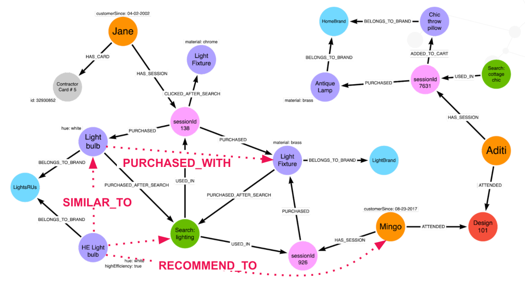
\includegraphics[width=0.9\linewidth,keepaspectratio]{gds4}
\end{center}

\end{frame}

%%%%%%%%%%%%%%%%%%%%%%%%%%%%%%%%%%%%%%%%%%%%%%%%%%%%%%%%%%%%%%%%%%%%%%%%%%%%%%%%%%
\begin{frame}[fragile]\frametitle{Any confusion?}

\begin{center}
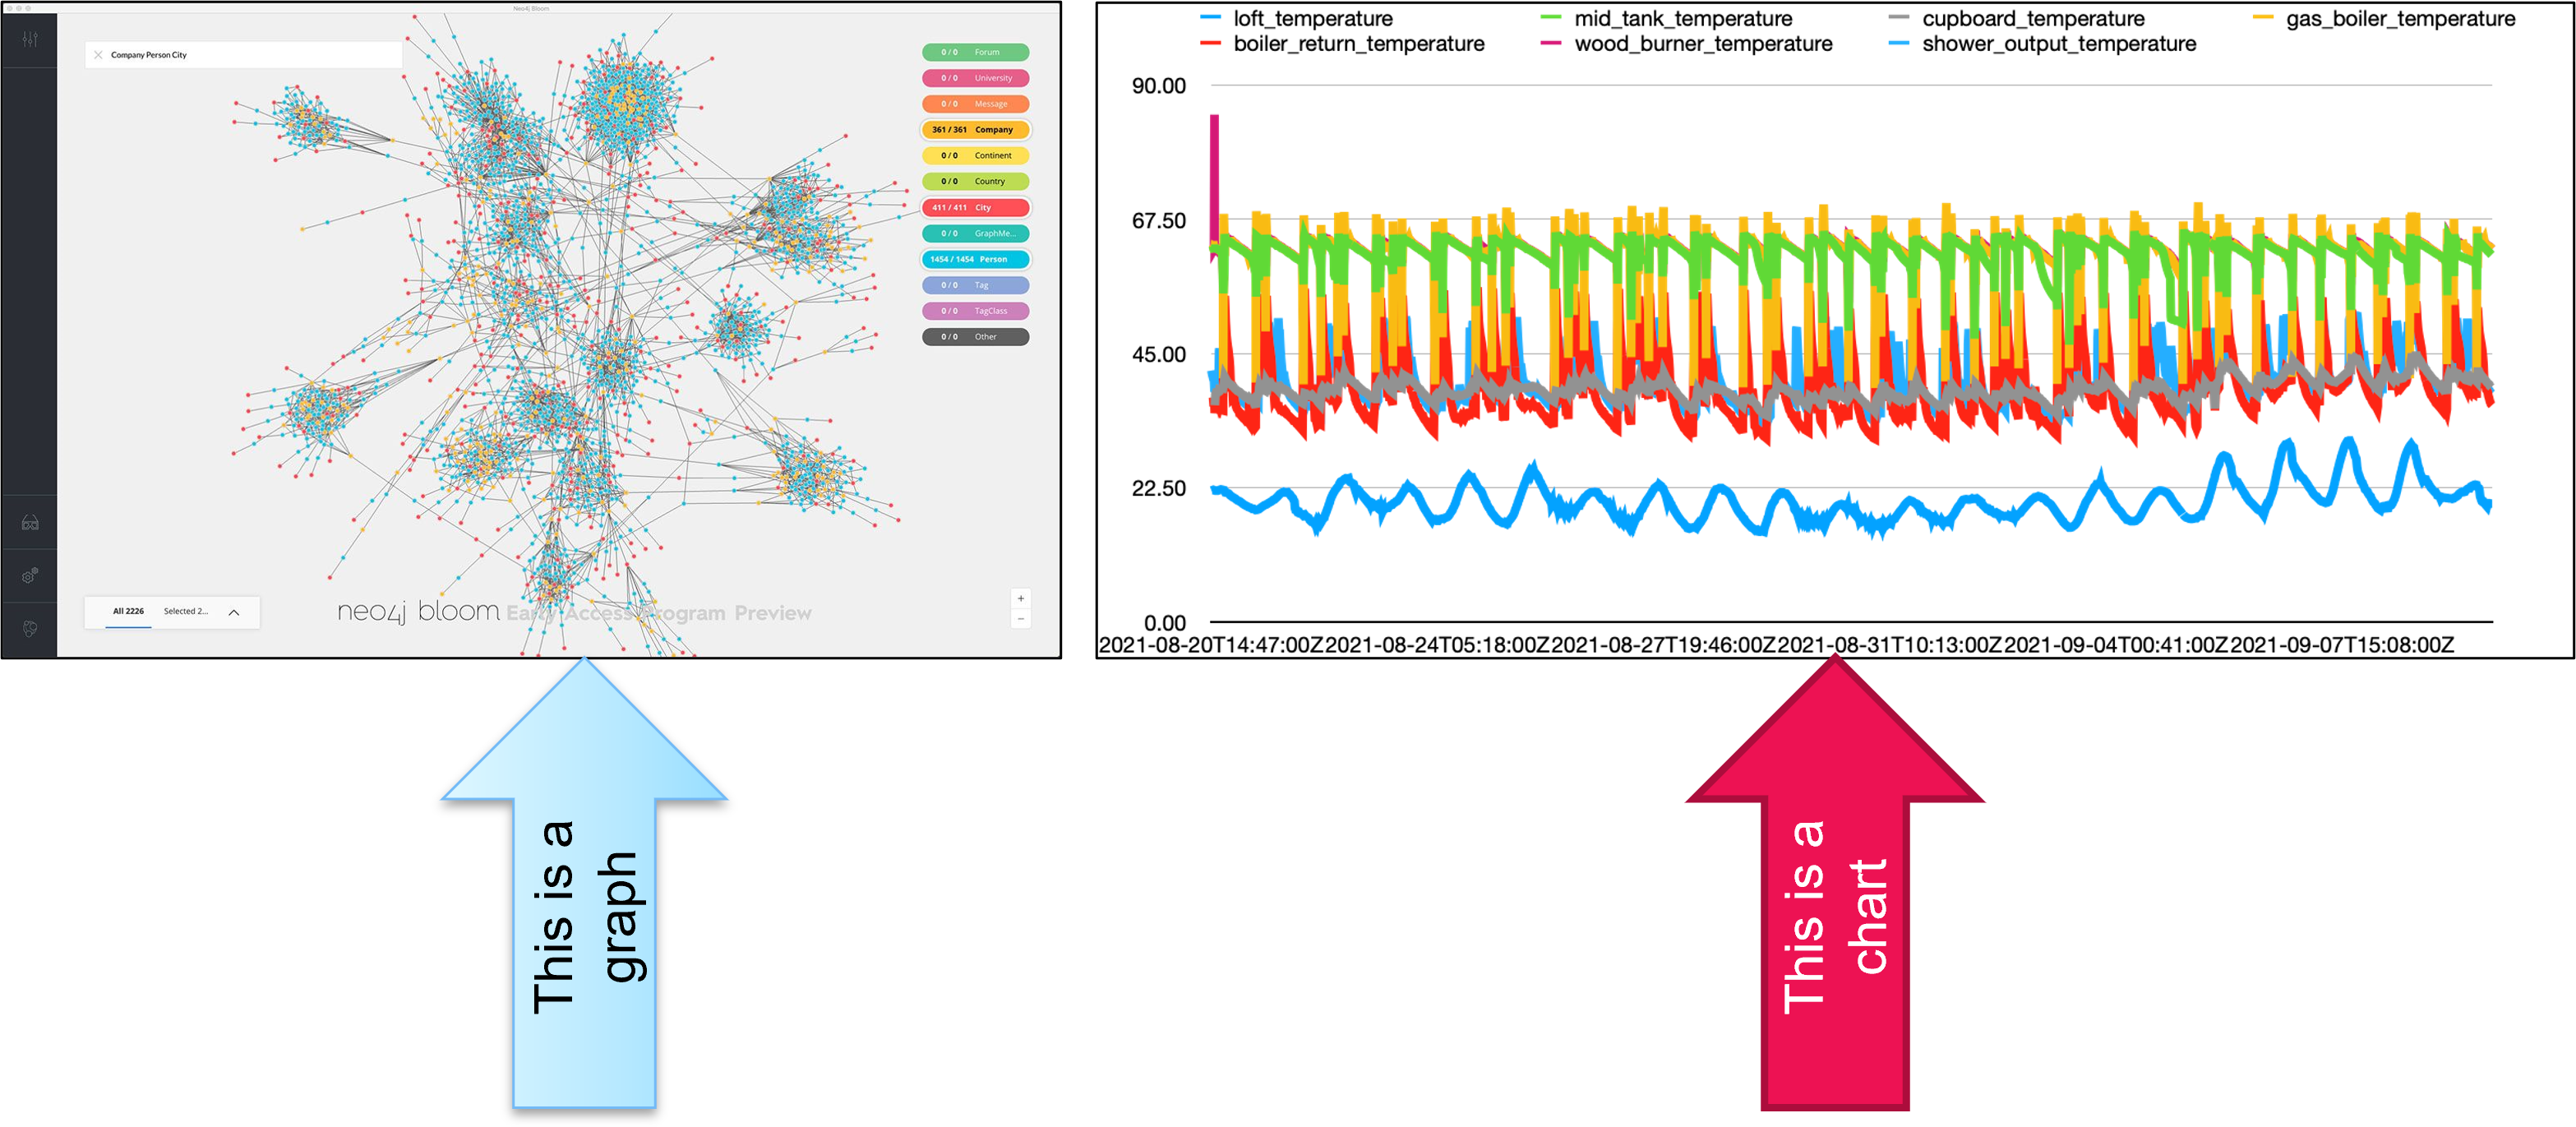
\includegraphics[width=\linewidth,keepaspectratio]{gds5}
\end{center}

\end{frame}

%%%%%%%%%%%%%%%%%%%%%%%%%%%%%%%%%%%%%%%%%%%%%%%%%%%%%%%%%%%%%%%%%%%%%%%%%%%%%%%%%%
\begin{frame}[fragile]\frametitle{Whats different?}

\begin{itemize}
\item Separate vs connected
\item Fixed vs variable size
\end{itemize}

\begin{center}
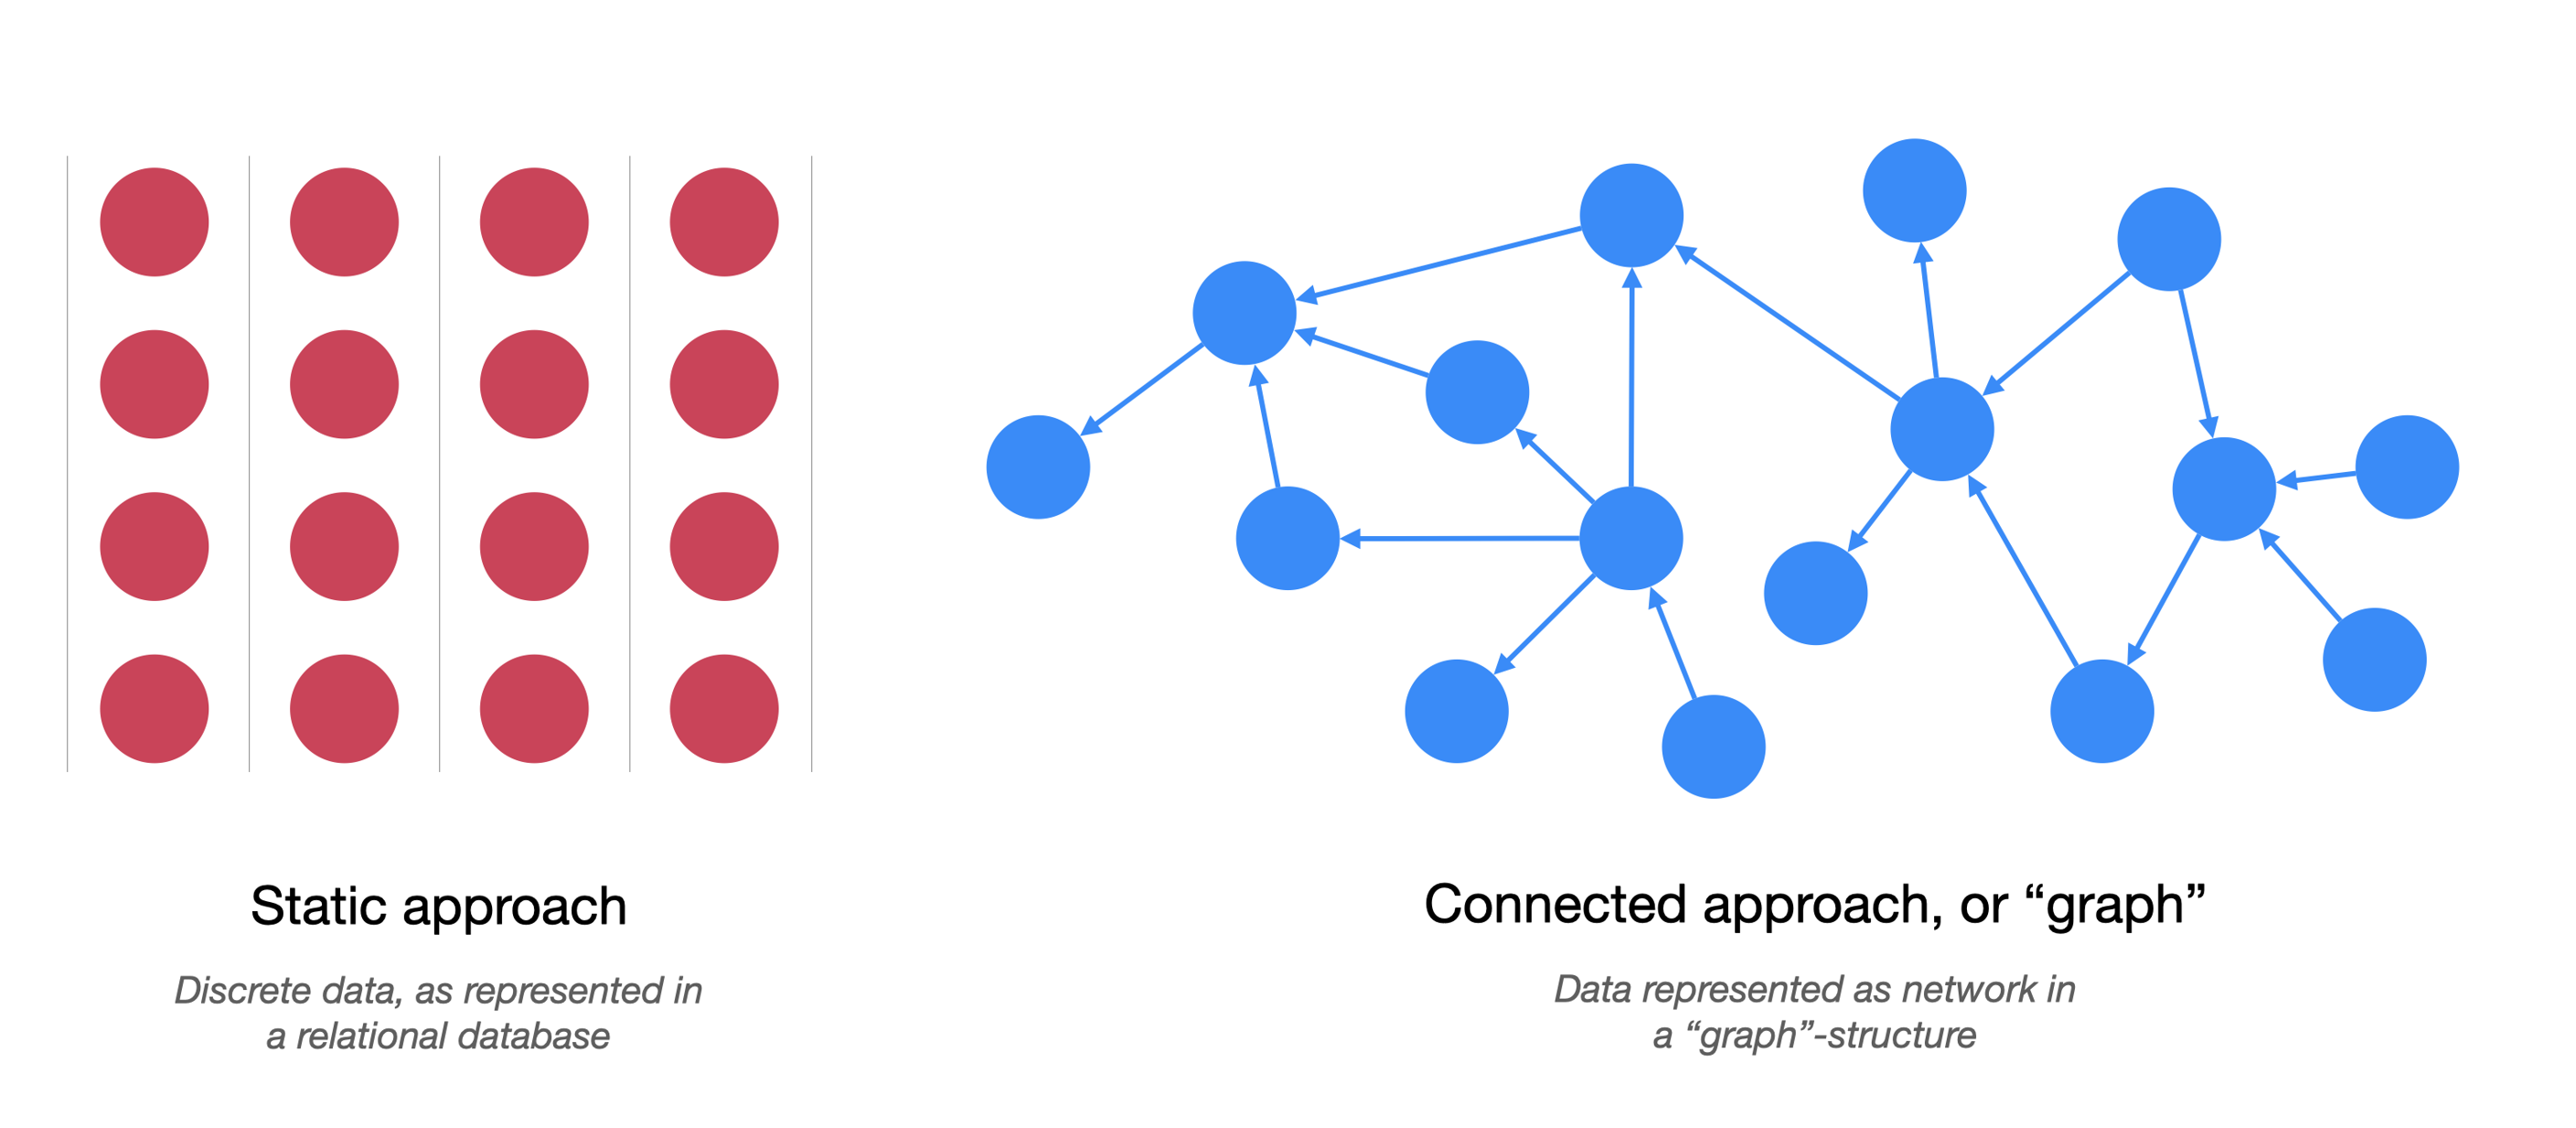
\includegraphics[width=\linewidth,keepaspectratio]{gds6}
\end{center}

\end{frame}

%%%%%%%%%%%%%%%%%%%%%%%%%%%%%%%%%%%%%%%%%%%%%%%%%%%%%%%%%%%%%%%%%%%%%%%%%%%%%%%%%%
\begin{frame}[fragile]\frametitle{What is data science?}

\begin{center}
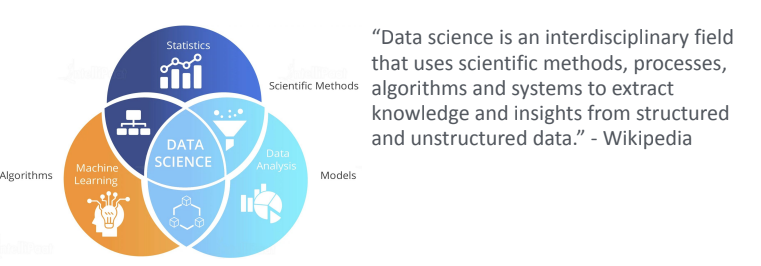
\includegraphics[width=\linewidth,keepaspectratio]{gds29}

{\tiny (Mark Needham - Intro to Graph Data Science with Neo4j)}

\end{center}

Data scientists use data to answer questions.

\end{frame}

%%%%%%%%%%%%%%%%%%%%%%%%%%%%%%%%%%%%%%%%%%%%%%%%%%%%%%%%%%%%%%%%%%%%%%%%%%%%%%%%%%
\begin{frame}[fragile]\frametitle{What is GRAPH data science?}

\begin{center}
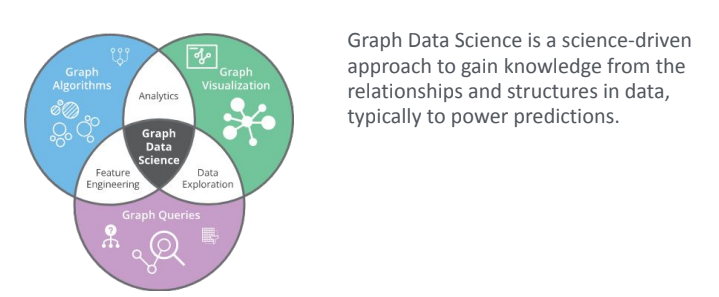
\includegraphics[width=\linewidth,keepaspectratio]{gds30}

{\tiny (Mark Needham - Intro to Graph Data Science with Neo4j)}

\end{center}

Data scientists use relationships to answer questions.
\end{frame}

%%%%%%%%%%%%%%%%%%%%%%%%%%%%%%%%%%%%%%%%%%%%%%%%%%%%%%%%%%%%%%%%%%%%%%%%%%%%%%%%%%
\begin{frame}[fragile]\frametitle{What is GRAPH data science?}

\begin{center}
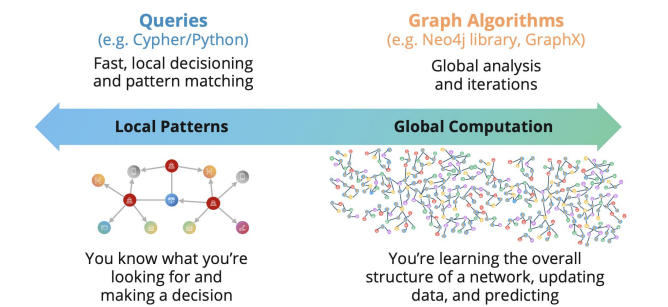
\includegraphics[width=\linewidth,keepaspectratio]{gds31}

{\tiny (Mark Needham - Intro to Graph Data Science with Neo4j)}

\end{center}

\end{frame}



%%%%%%%%%%%%%%%%%%%%%%%%%%%%%%%%%%%%%%%%%%%%%%%%%%%%%%%%%%%%%%%%%%%%%%%%%%%%%%%%%%
\begin{frame}[fragile]\frametitle{Graphs enrich all stages of Data Science}

\begin{center}
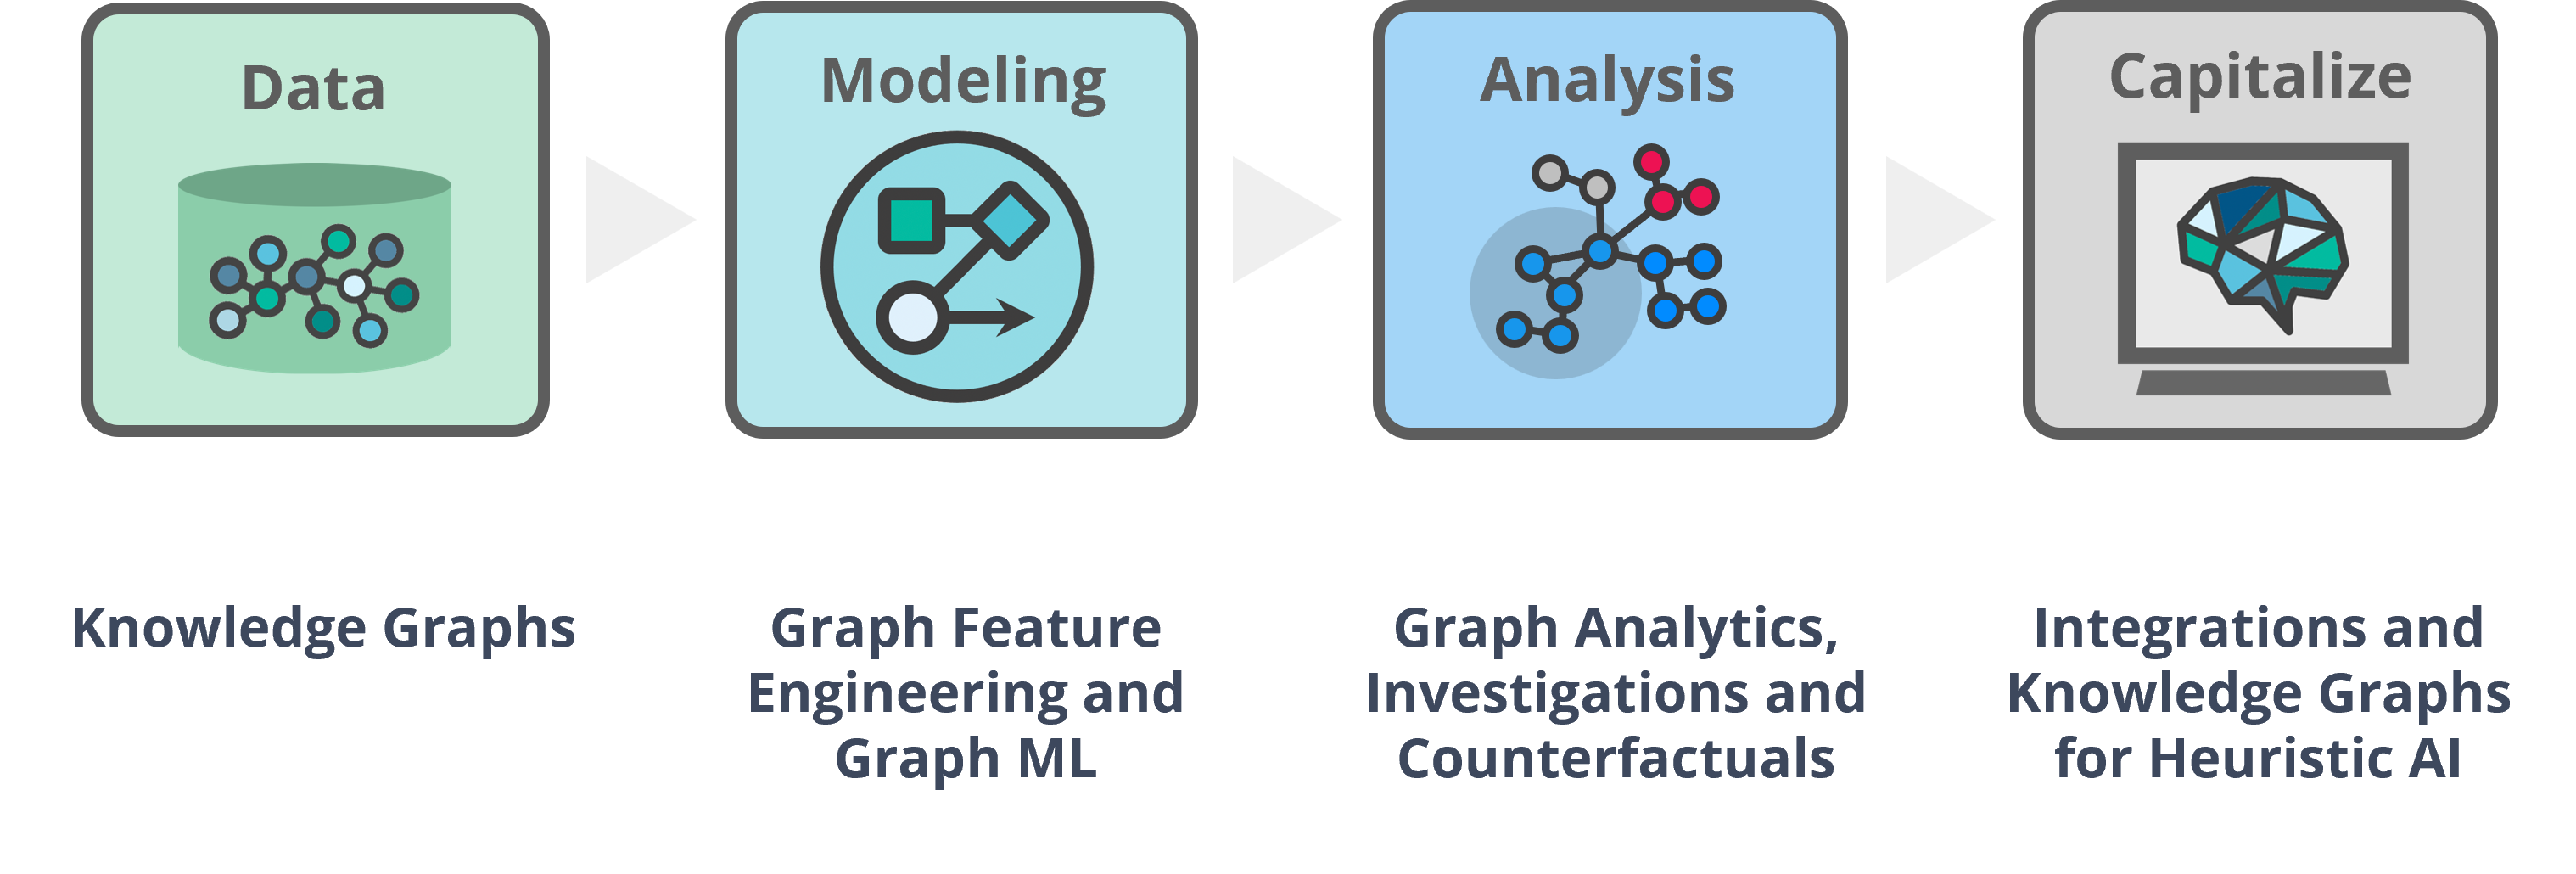
\includegraphics[width=\linewidth,keepaspectratio]{gds7}
\end{center}

\end{frame}


%%%%%%%%%%%%%%%%%%%%%%%%%%%%%%%%%%%%%%%%%%%%%%%%%%%%%%%%%%%%%%%%%%%%%%%%%%%%%%%%%%
\begin{frame}[fragile]\frametitle{Graph Data Science}

\begin{center}
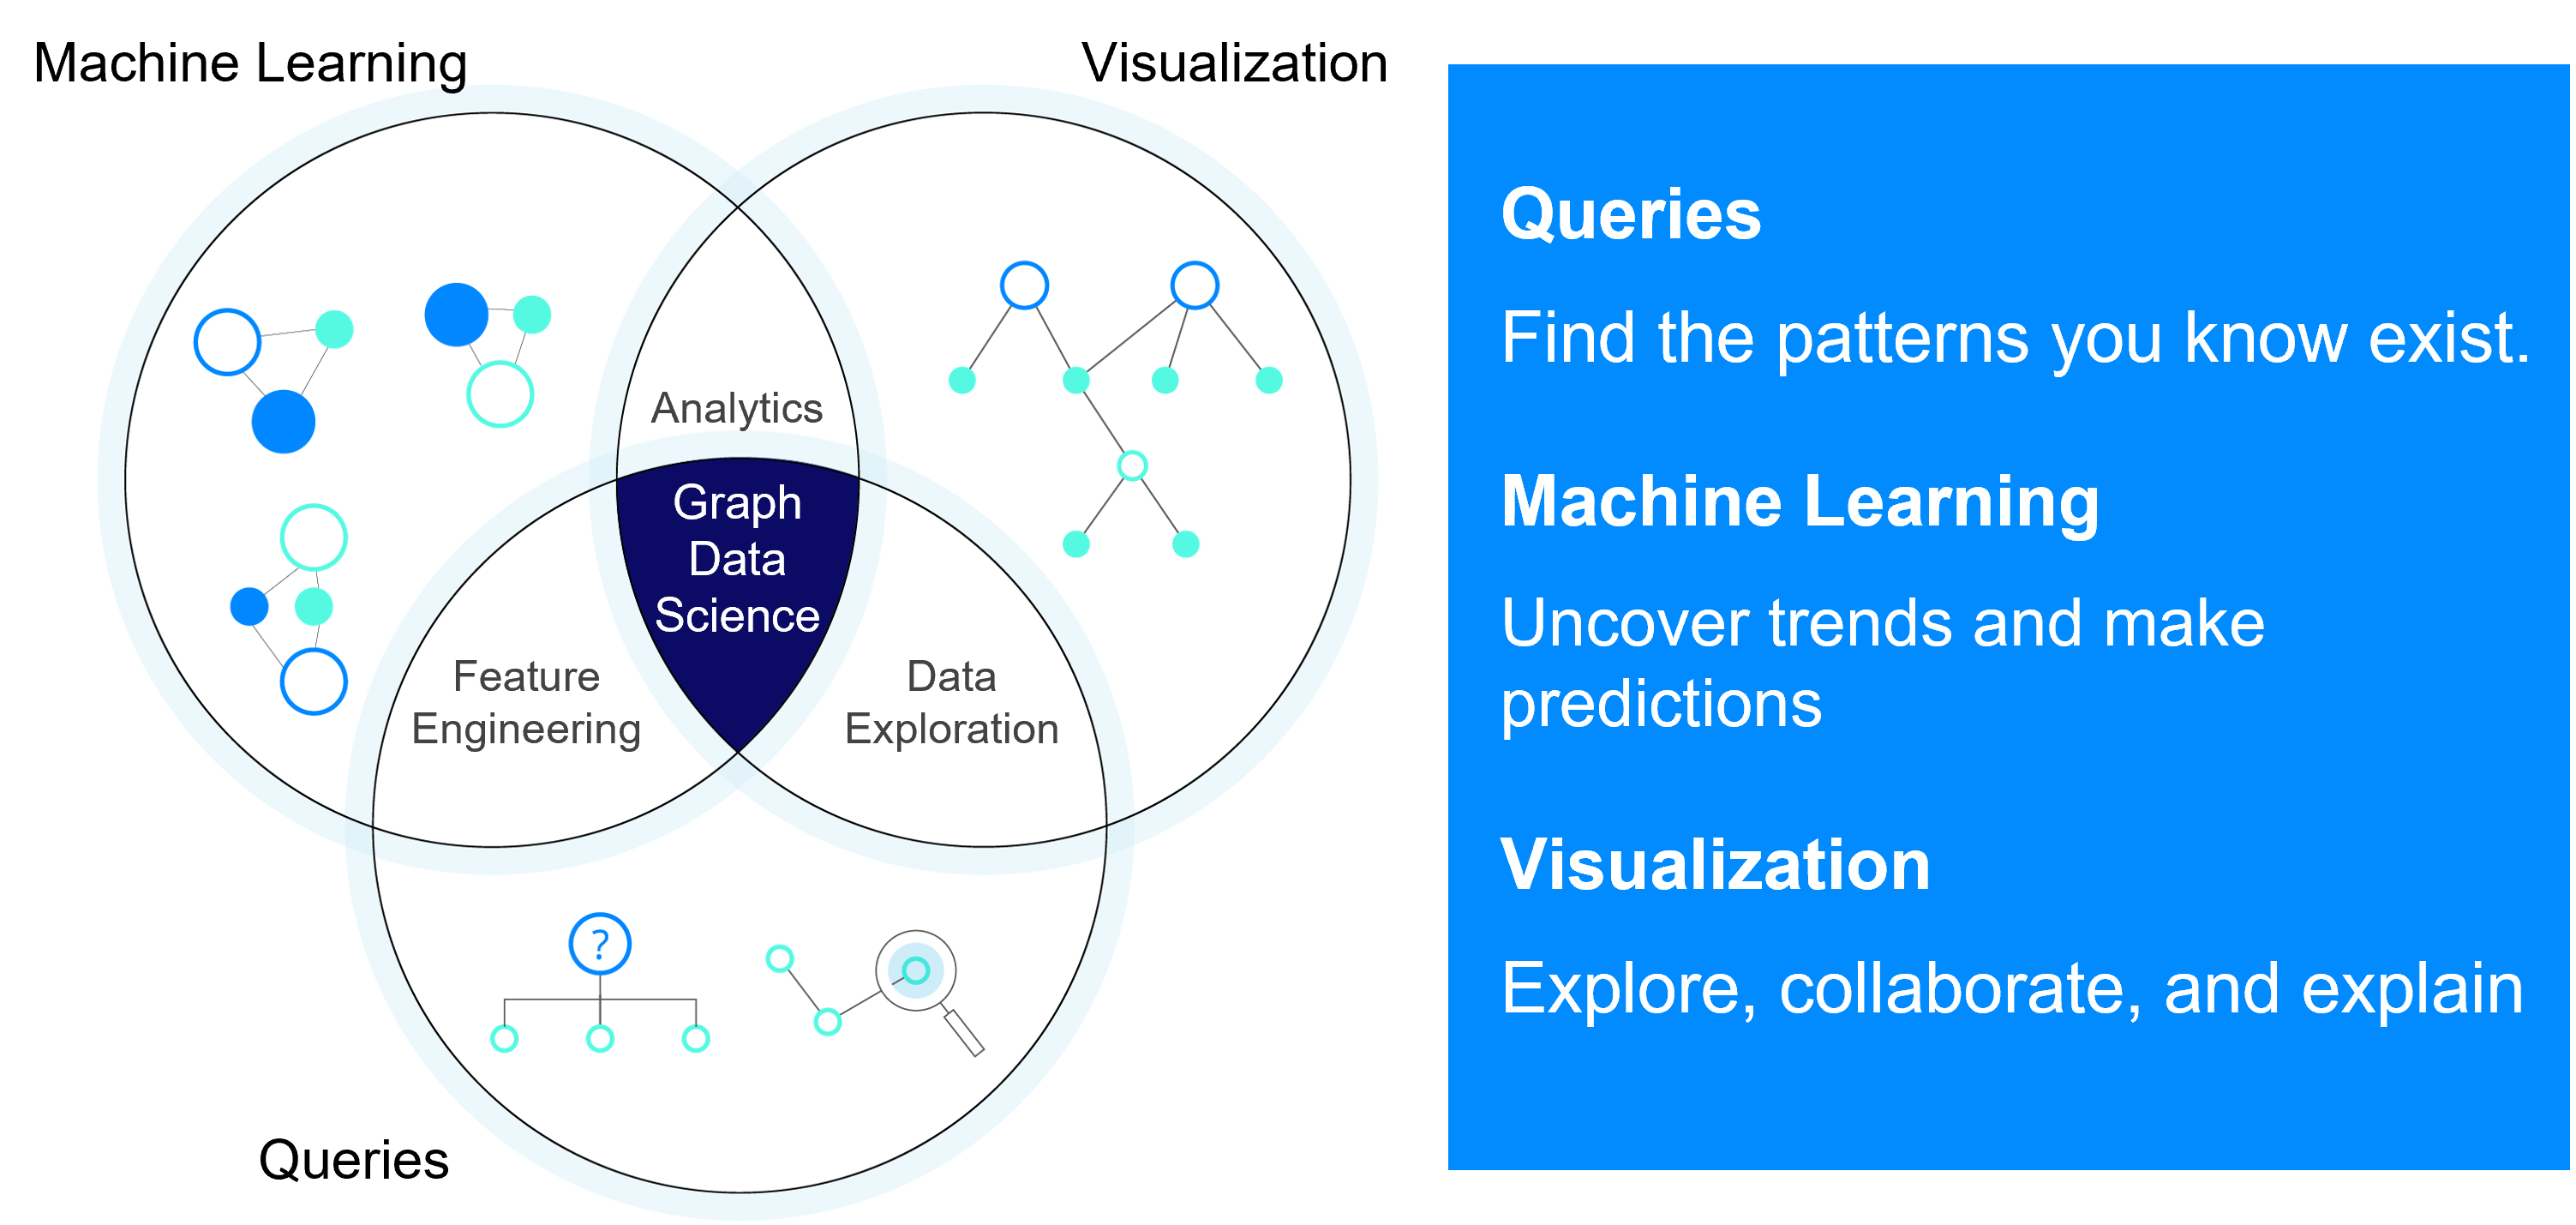
\includegraphics[width=\linewidth,keepaspectratio]{gds8}
\end{center}

\end{frame}

%%%%%%%%%%%%%%%%%%%%%%%%%%%%%%%%%%%%%%%%%%%%%%%%%%%%%%%%%%%%%%%%%%%%%%%%%%%%%%%%%%
\begin{frame}[fragile]\frametitle{Graph Data Science Applications}

\begin{center}
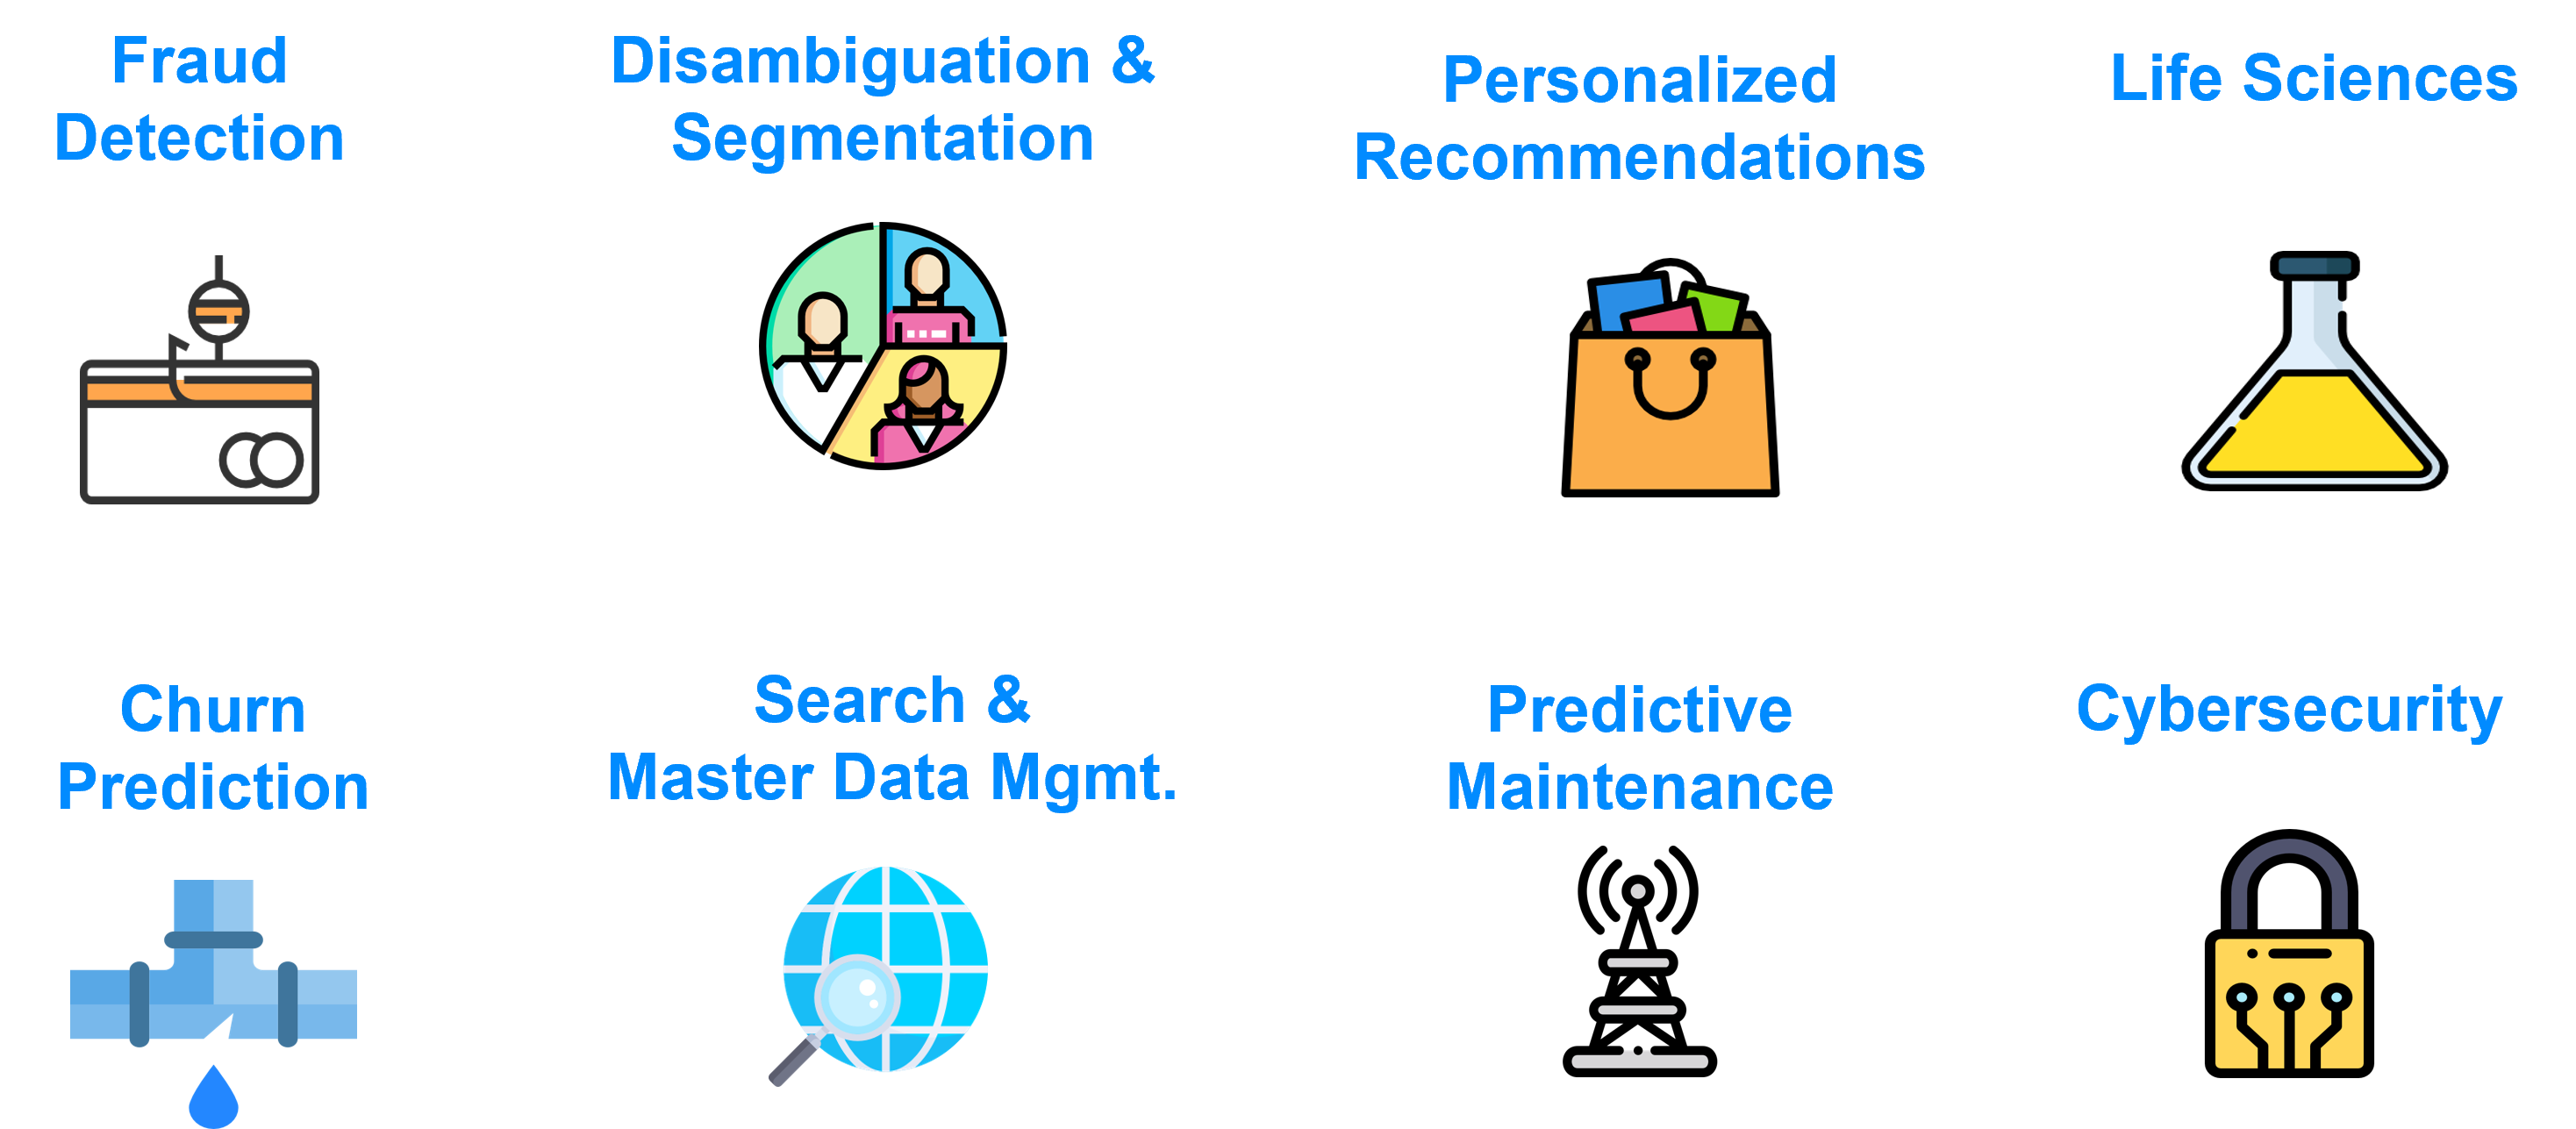
\includegraphics[width=\linewidth,keepaspectratio]{gds9}
\end{center}

\end{frame}

%%%%%%%%%%%%%%%%%%%%%%%%%%%%%%%%%%%%%%%%%%%%%%%%%%%%%%%%%%%%%%%%%%%%%%%%%%%%%%%%%%
\begin{frame}[fragile]\frametitle{Graph Data Science}

\begin{center}
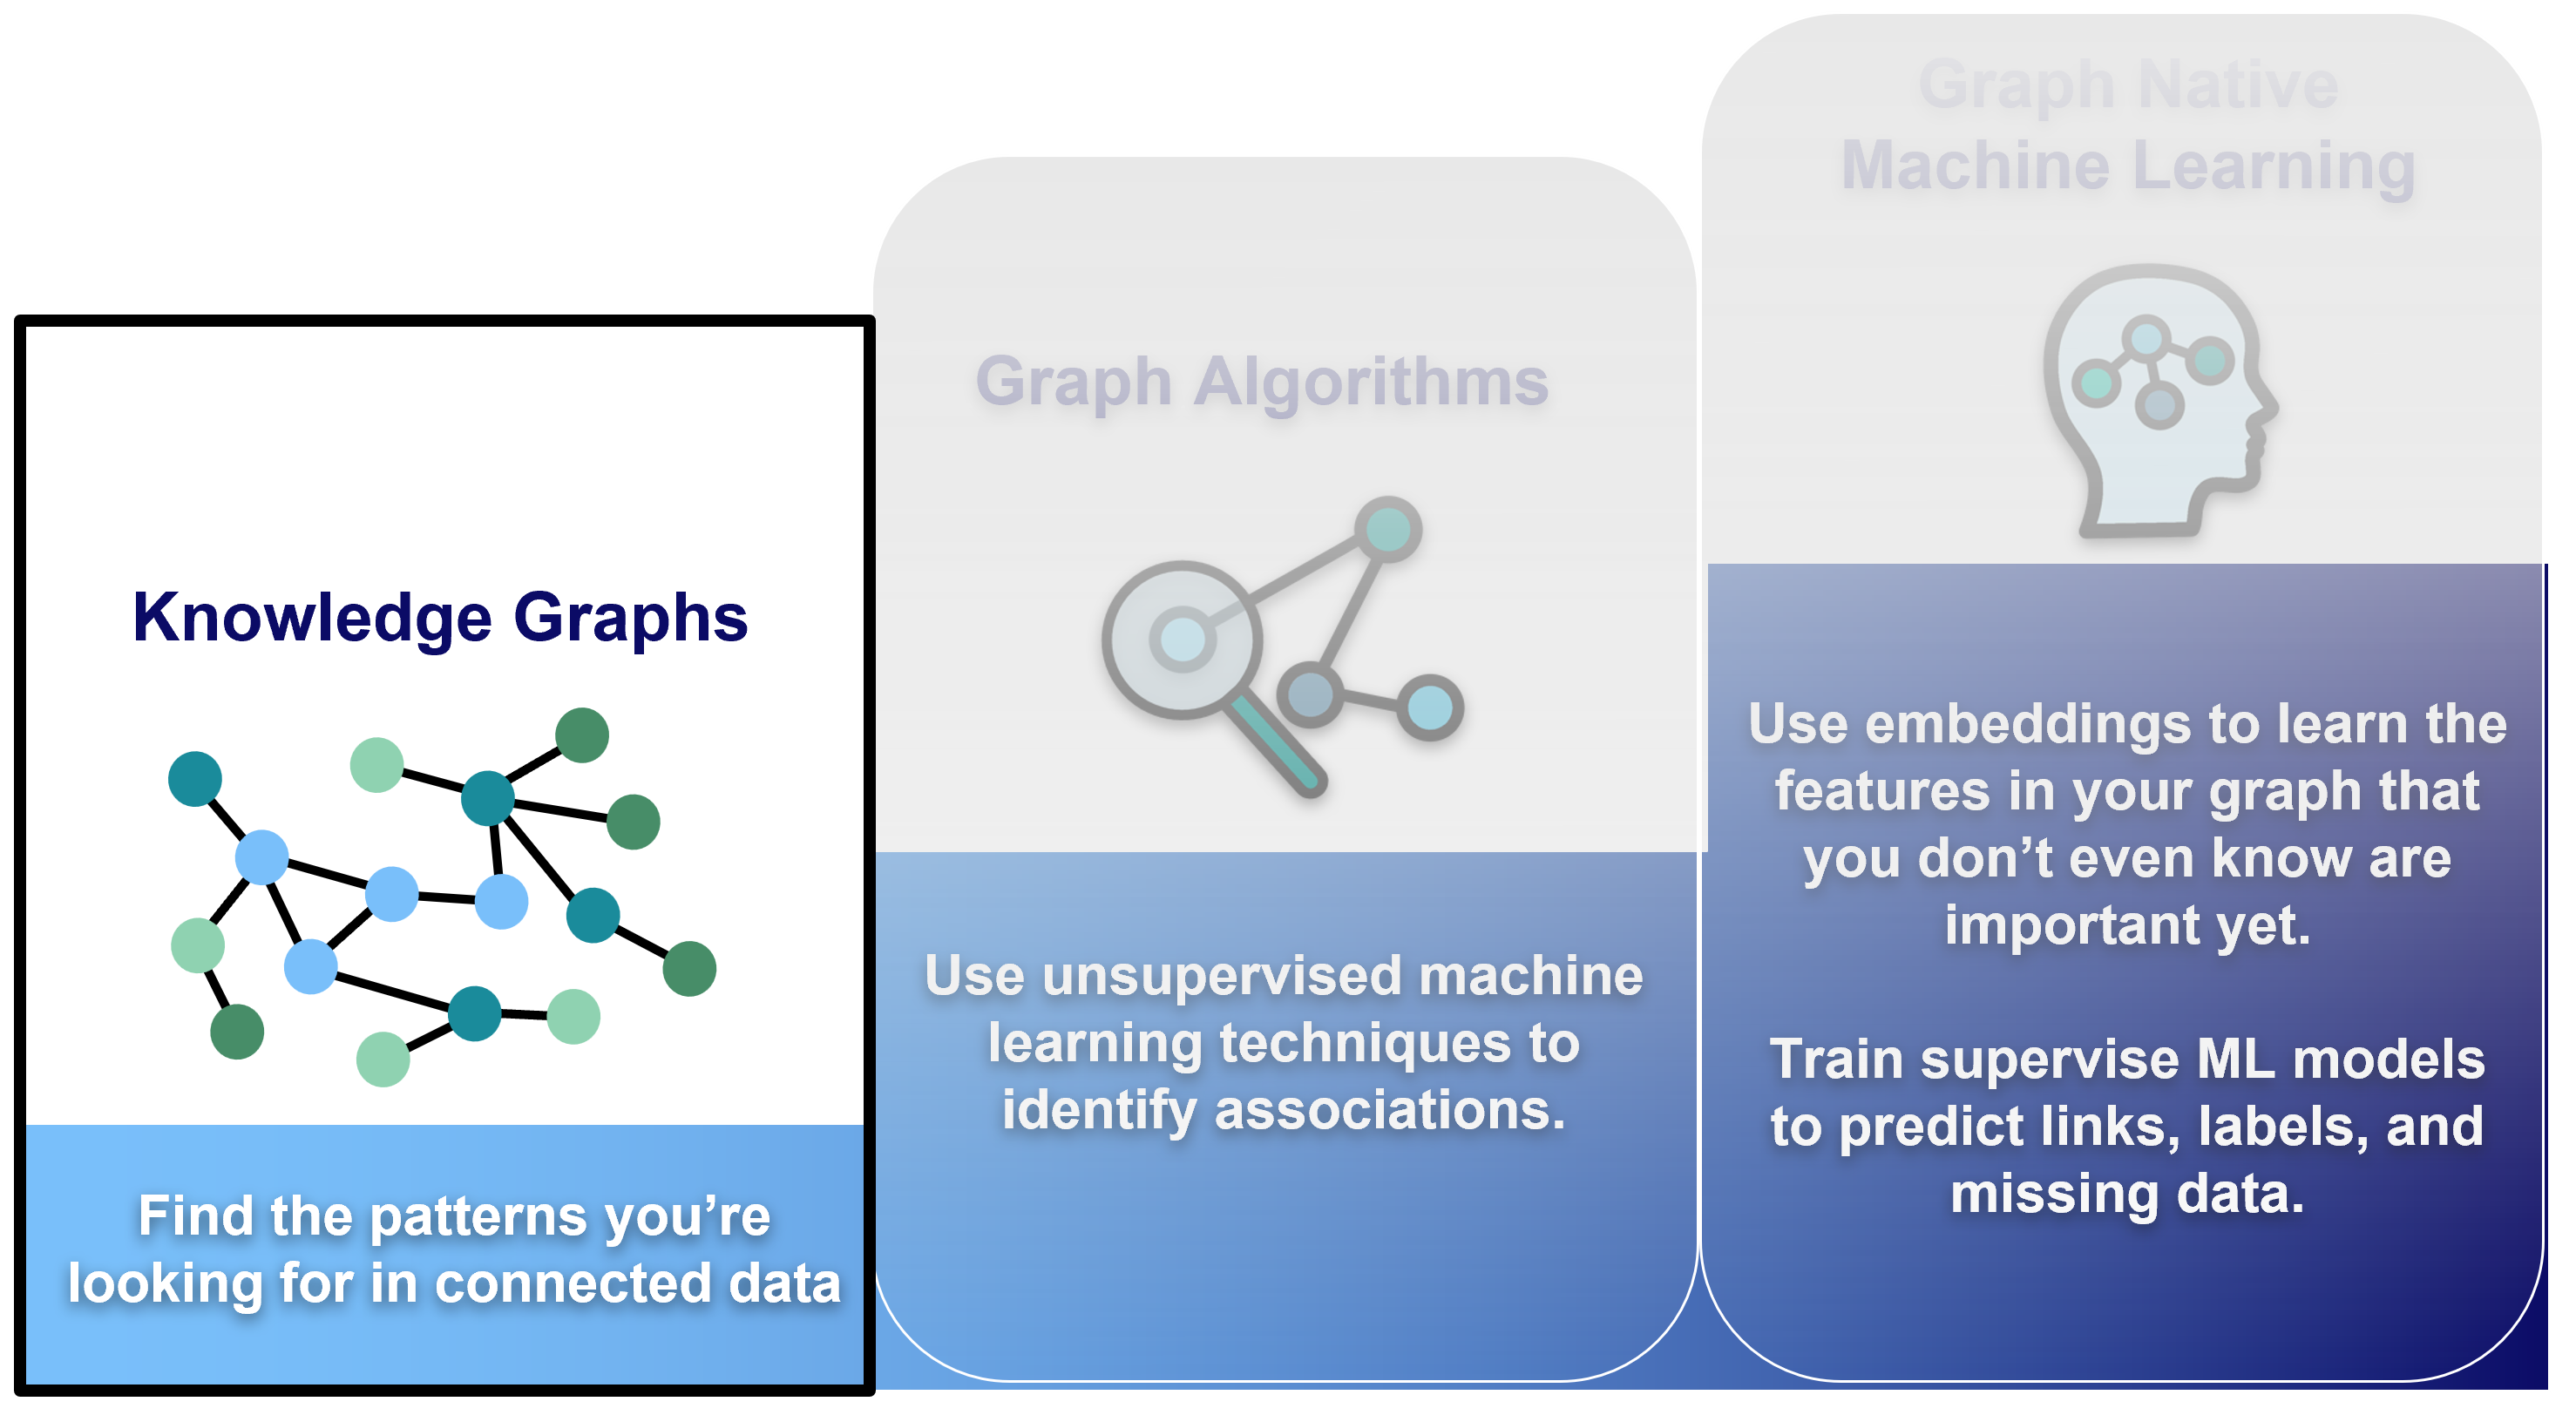
\includegraphics[width=\linewidth,keepaspectratio]{gds10}
\end{center}

\end{frame}

%%%%%%%%%%%%%%%%%%%%%%%%%%%%%%%%%%%%%%%%%%%%%%%%%%%%%%%%%%%%%%%%%%%%%%%%%%%%%%%%%%
\begin{frame}[fragile]\frametitle{Knowledge Graph - Building Blocks}

\begin{center}
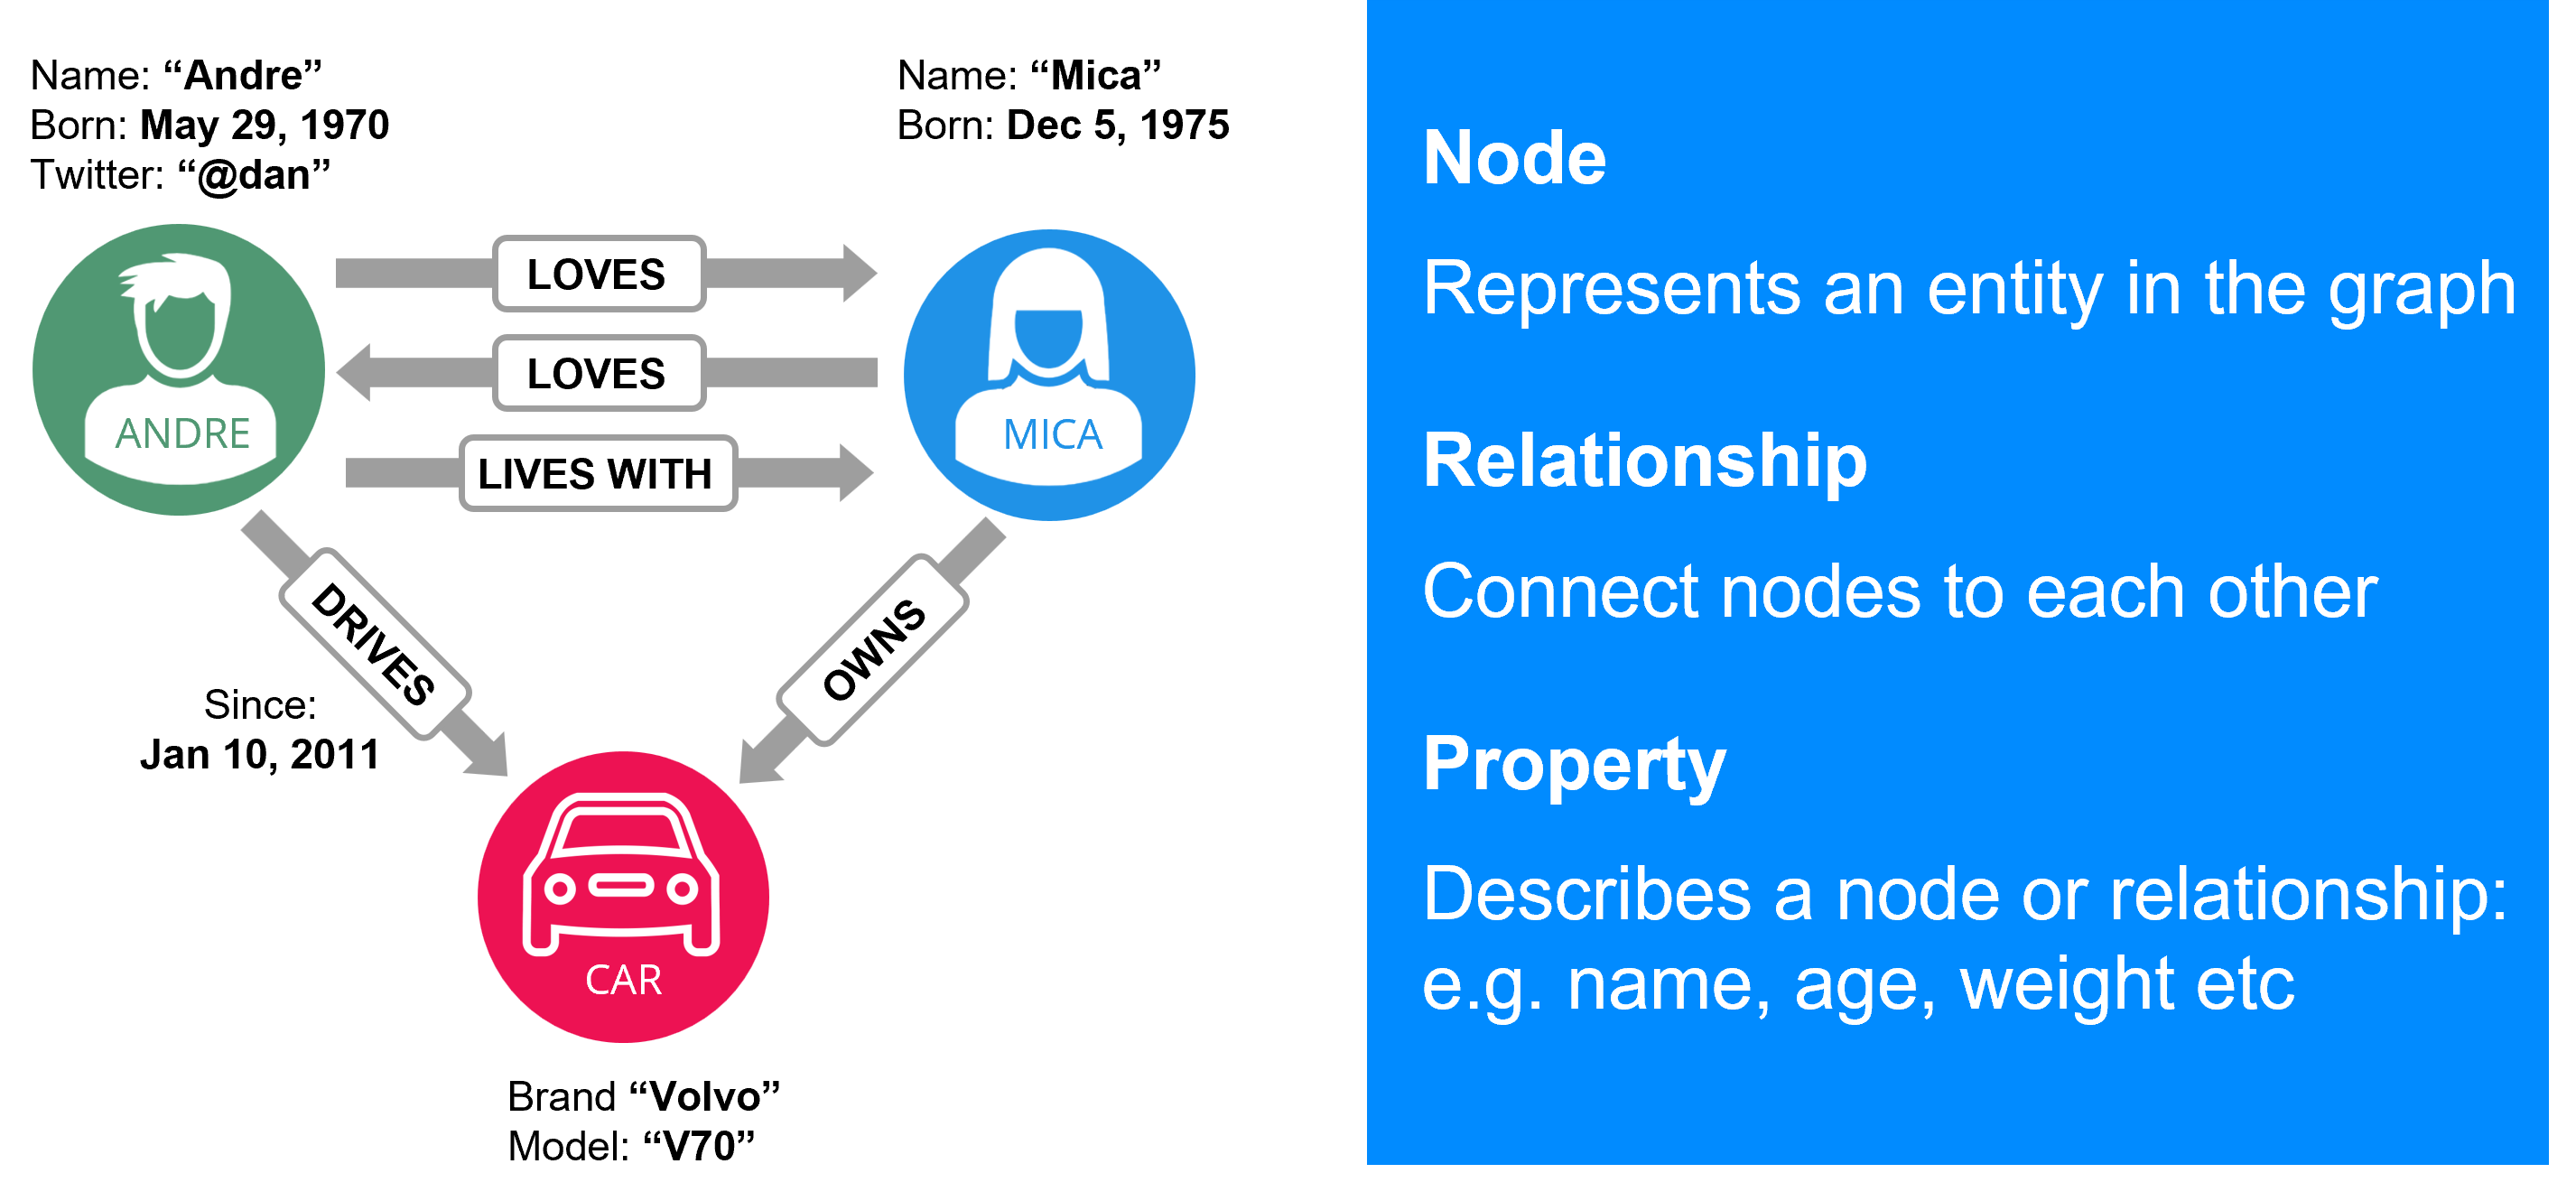
\includegraphics[width=\linewidth,keepaspectratio]{gds11}
\end{center}

\end{frame}

%%%%%%%%%%%%%%%%%%%%%%%%%%%%%%%%%%%%%%%%%%%%%%%%%%%%%%%%%%%%%%%%%%%%%%%%%%%%%%%%%%
\begin{frame}[fragile]\frametitle{Database, Query Language and Visualization}

\begin{center}
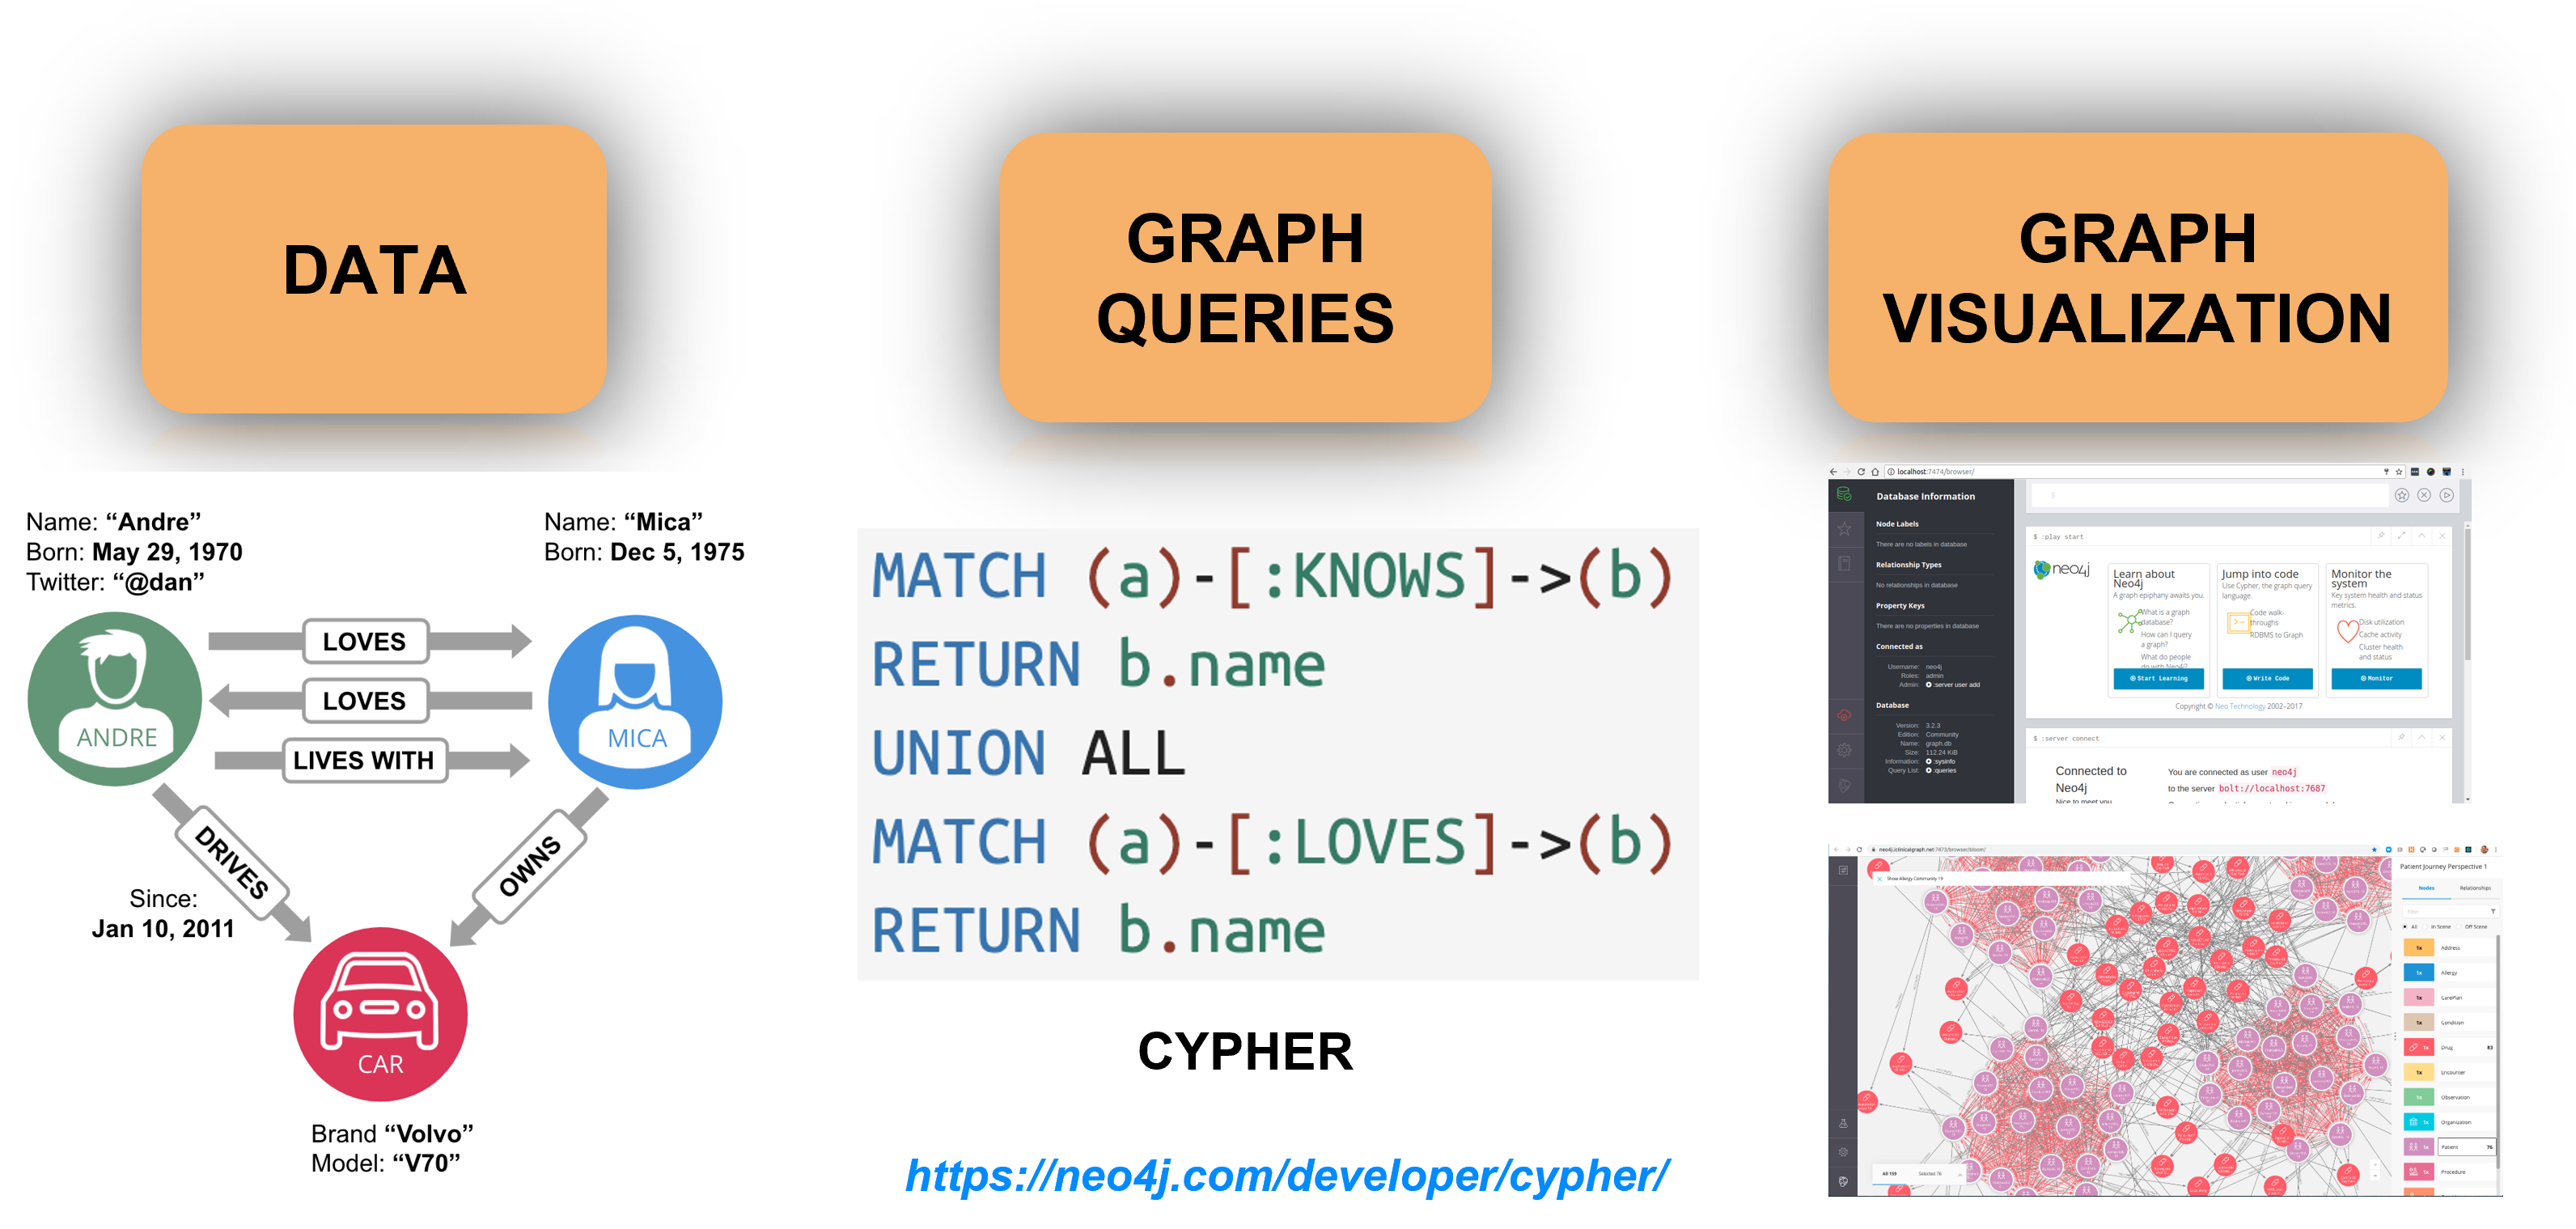
\includegraphics[width=\linewidth,keepaspectratio]{gds12}
\end{center}

\end{frame}

%%%%%%%%%%%%%%%%%%%%%%%%%%%%%%%%%%%%%%%%%%%%%%%%%%%%%%%%%%%%%%%%%%%%%%%%%%%%%%%%%%
\begin{frame}[fragile]\frametitle{What can you do with a knowledge graph?}

\begin{center}
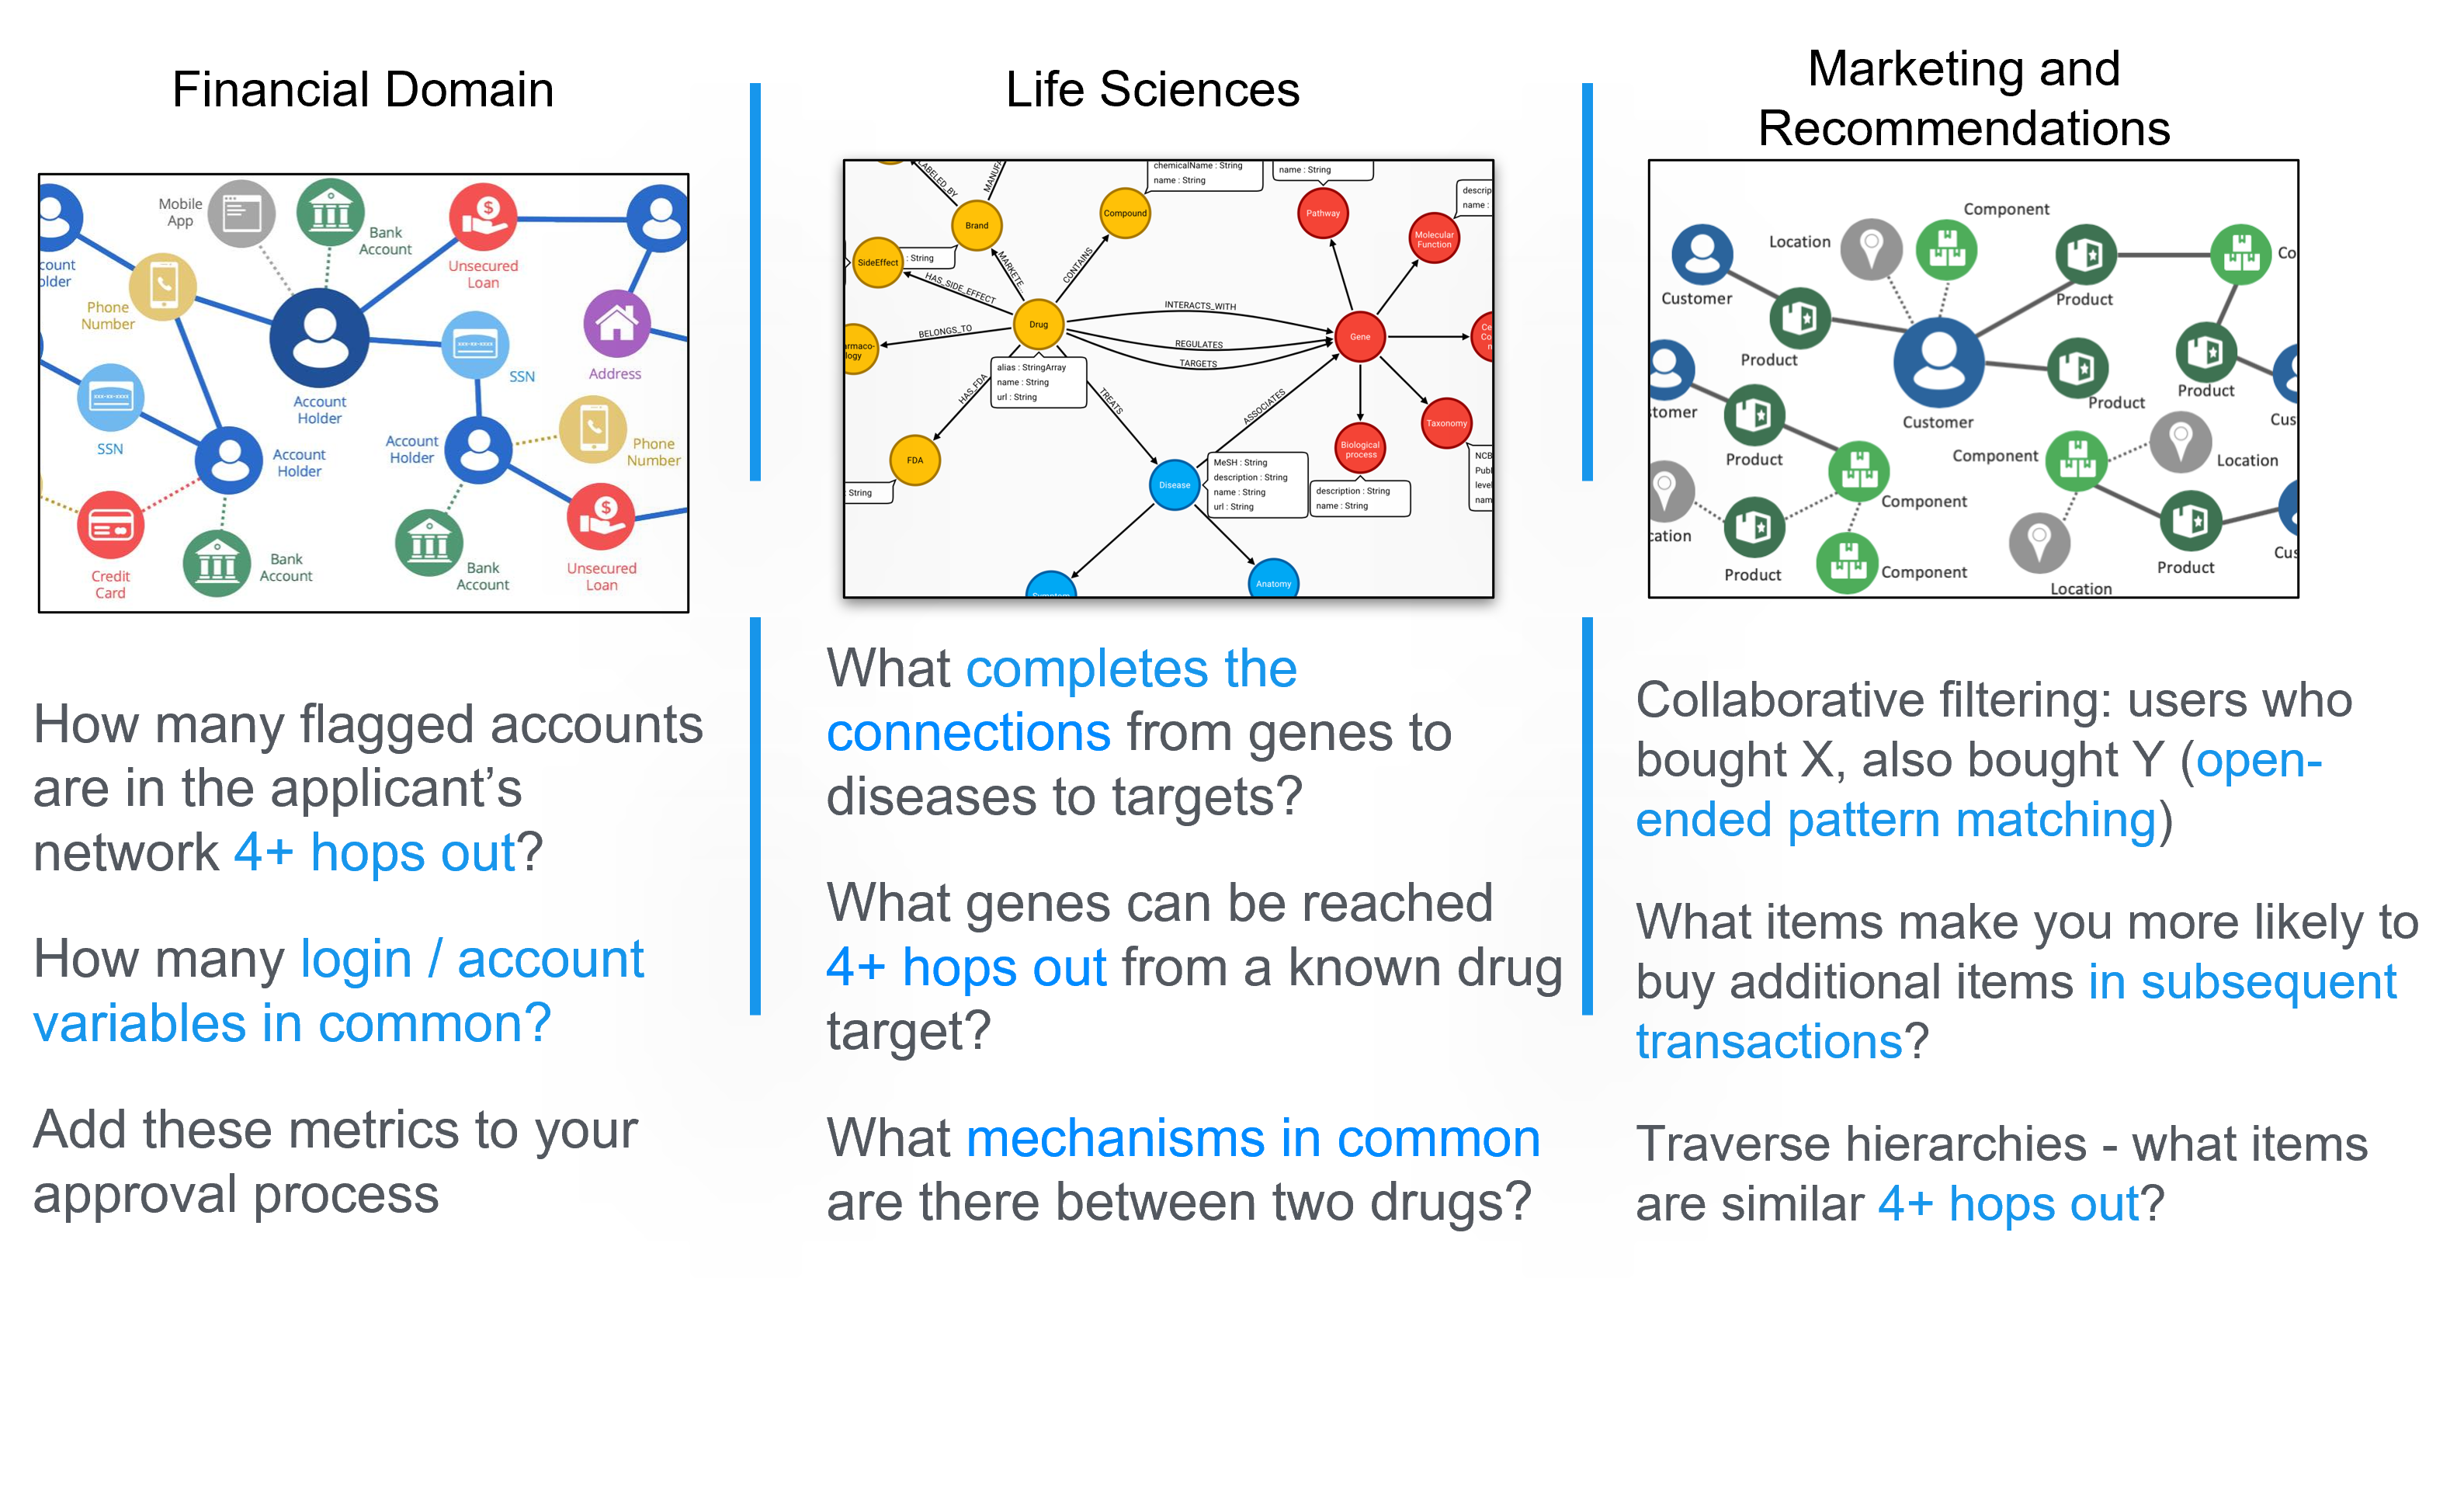
\includegraphics[width=\linewidth,keepaspectratio]{gds13}
\end{center}

\end{frame}

%%%%%%%%%%%%%%%%%%%%%%%%%%%%%%%%%%%%%%%%%%%%%%%%%%%%%%%%%%%%%%%%%%%%%%%%%%%%%%%%%%
\begin{frame}[fragile]\frametitle{Supply Chain: Organizational Knowledge graph}

\begin{center}
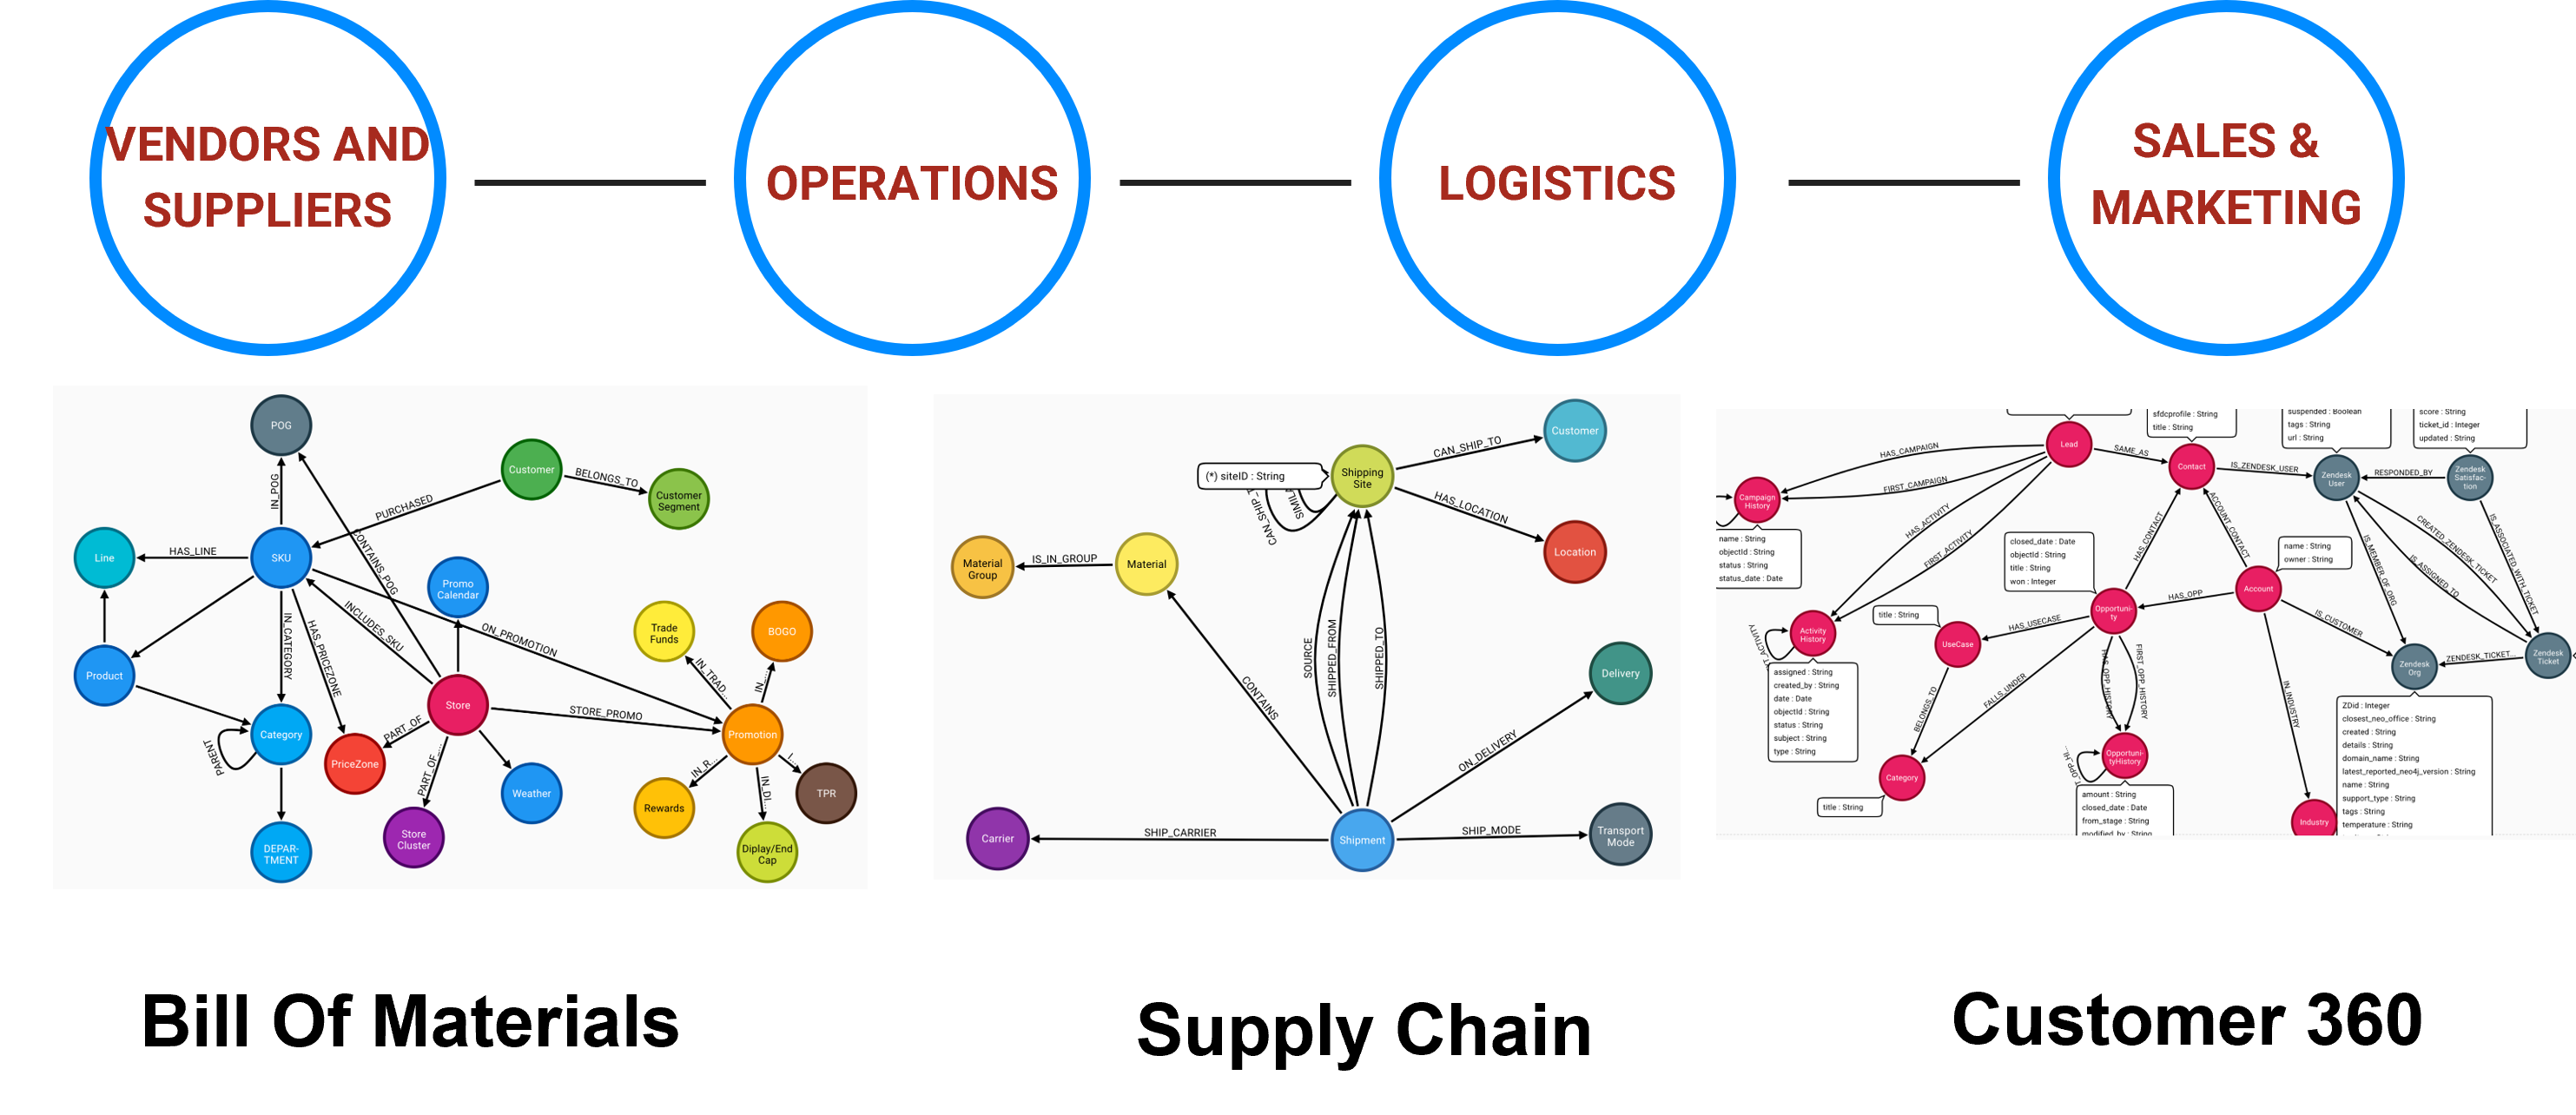
\includegraphics[width=\linewidth,keepaspectratio]{gds14}
\end{center}

\end{frame}

%%%%%%%%%%%%%%%%%%%%%%%%%%%%%%%%%%%%%%%%%%%%%%%%%%%%%%%%%%%%%%%%%%%%%%%%%%%%%%%%%%
\begin{frame}[fragile]\frametitle{Graph Data Science}

\begin{center}
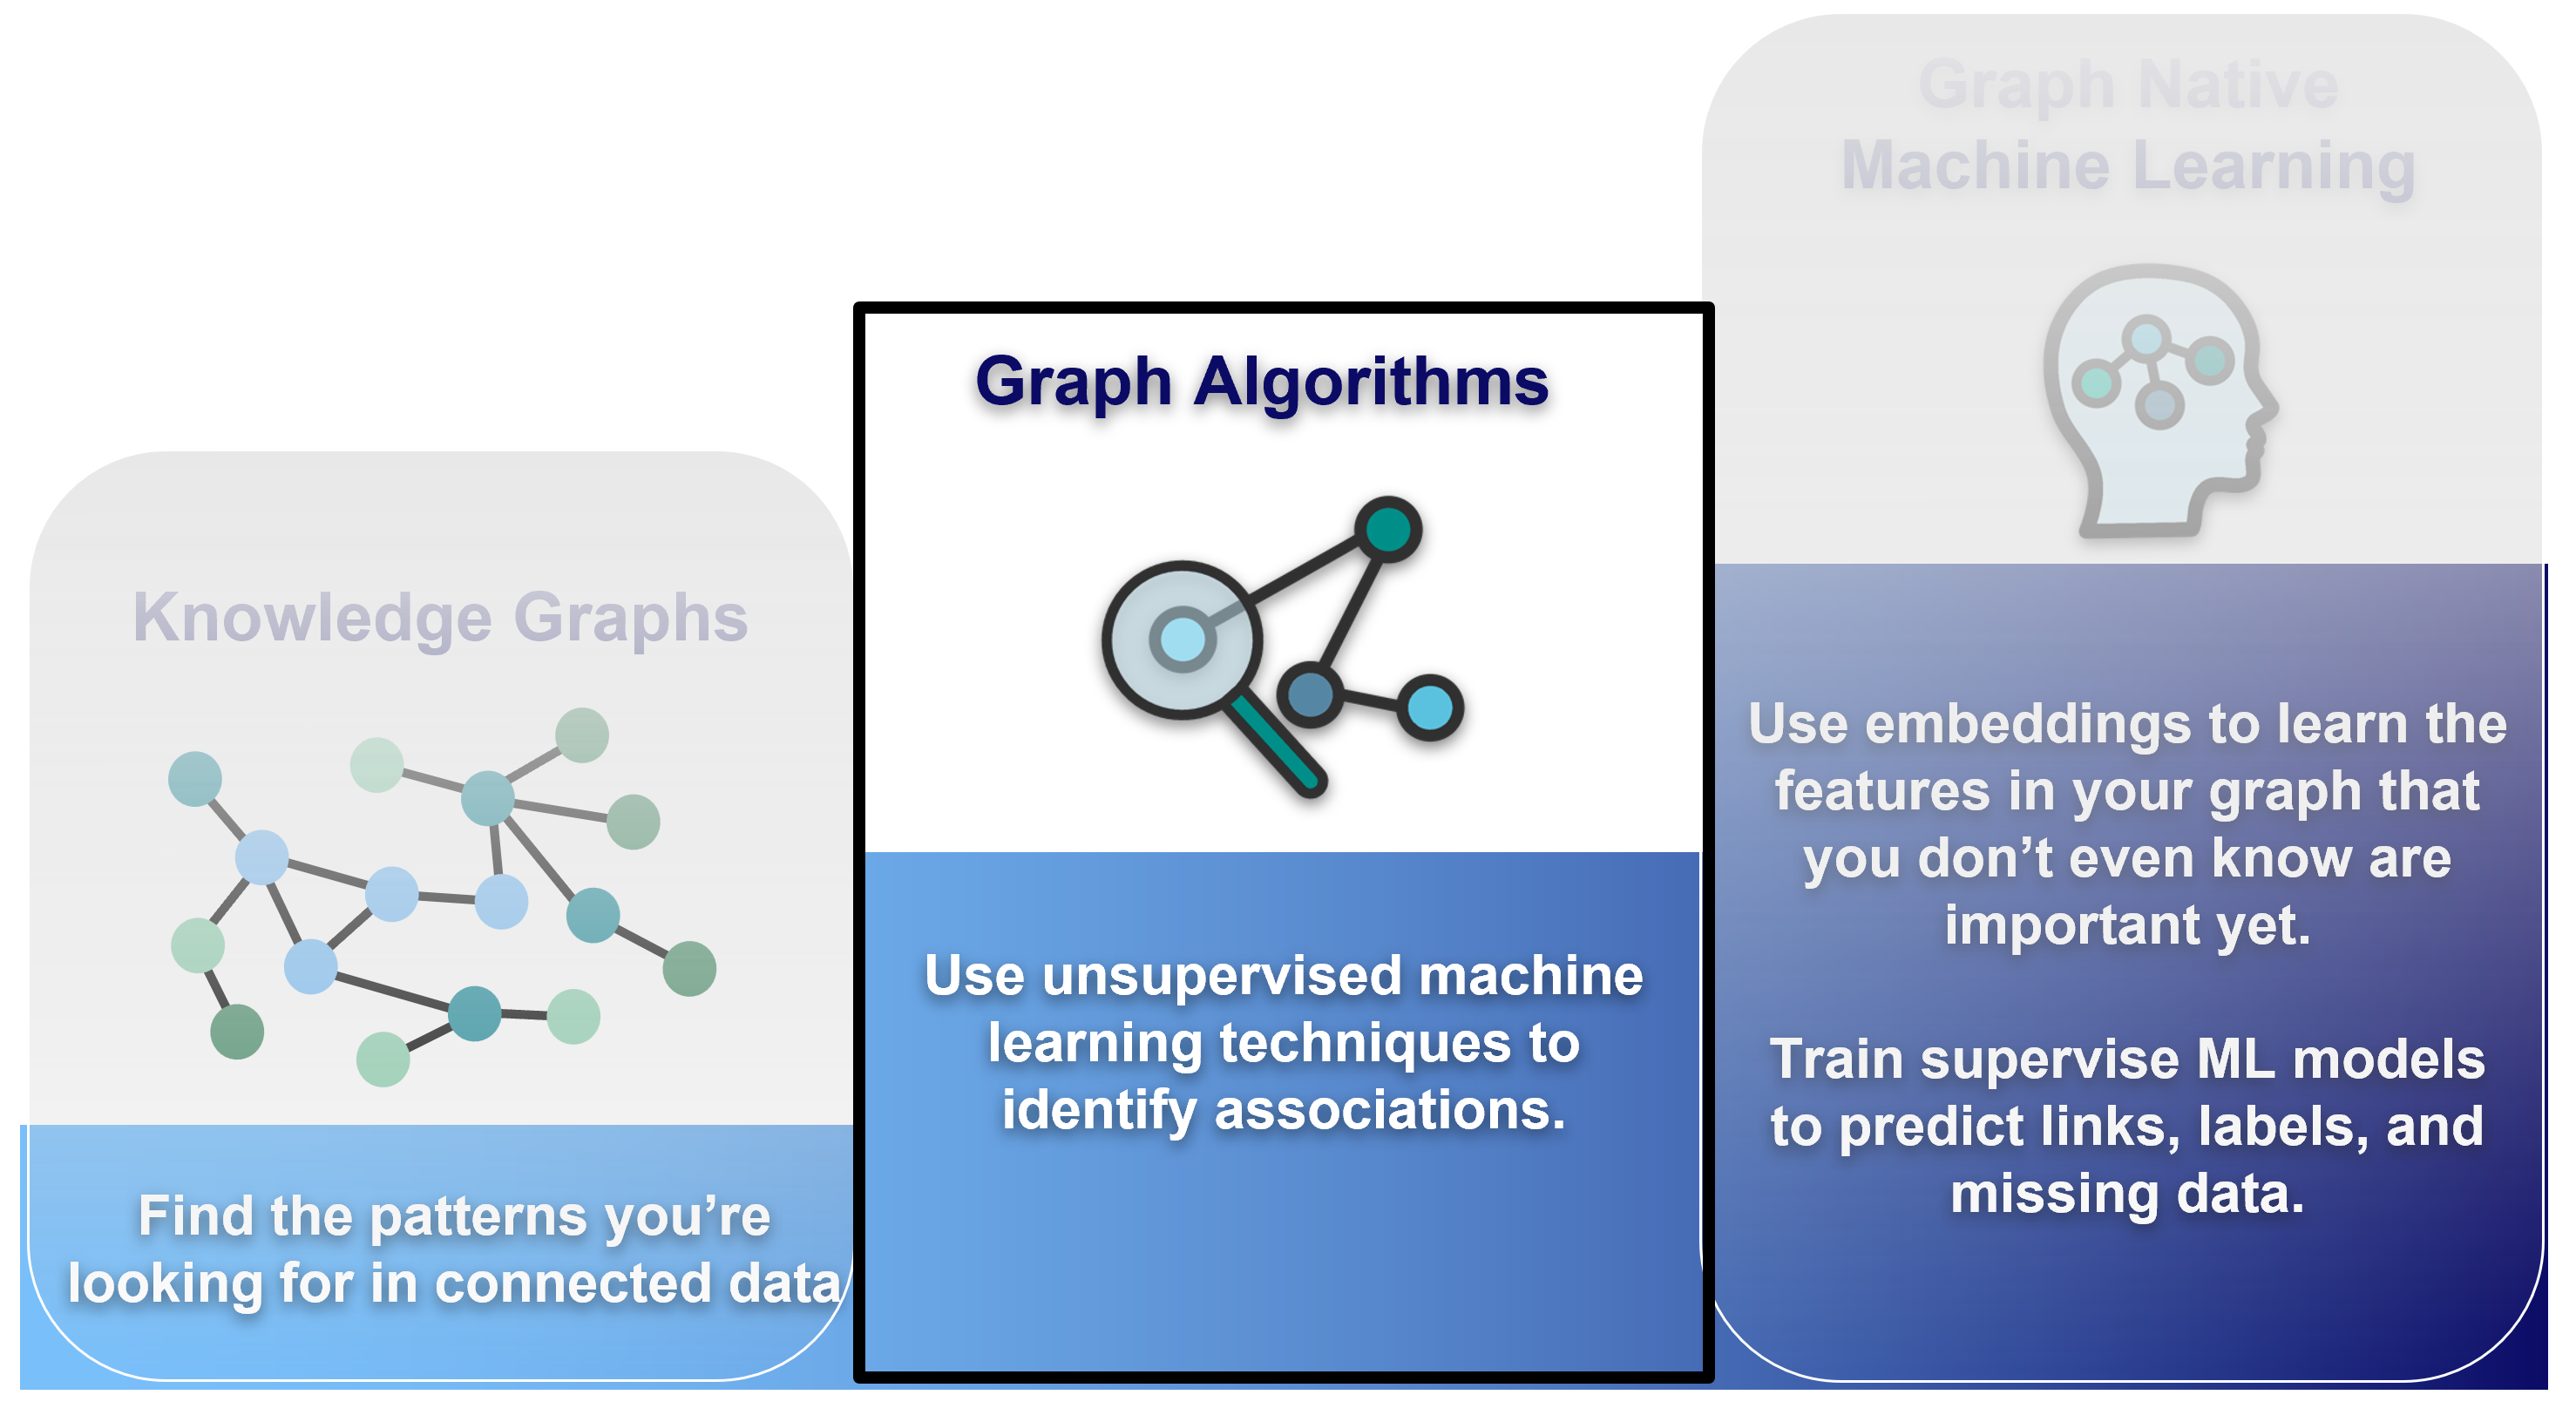
\includegraphics[width=\linewidth,keepaspectratio]{gds15}
\end{center}

\end{frame}

%%%%%%%%%%%%%%%%%%%%%%%%%%%%%%%%%%%%%%%%%%%%%%%%%%%%%%%%%%%%%%%%%%%%%%%%%%%%%%%%%%
\begin{frame}[fragile]\frametitle{Graph Algorithm types}

\begin{center}
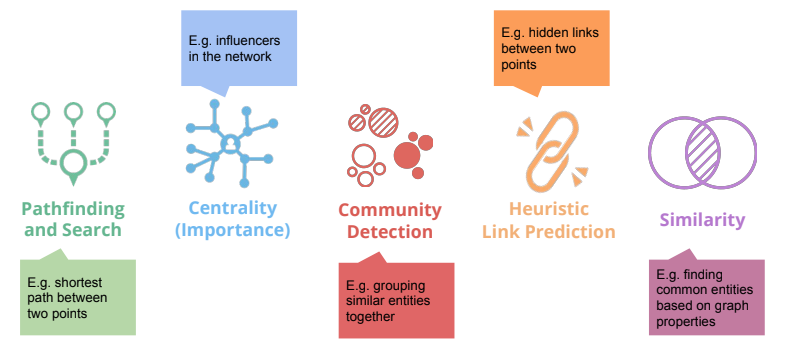
\includegraphics[width=\linewidth,keepaspectratio]{gds34}

{\tiny (Mark Needham - Intro to Graph Data Science with Neo4j)}

\end{center}

\end{frame}


%%%%%%%%%%%%%%%%%%%%%%%%%%%%%%%%%%%%%%%%%%%%%%%%%%%%%%%%%%%%%%%%%%%%%%%%%%%%%%%%%%
\begin{frame}[fragile]\frametitle{Graph Algorithms}

\begin{center}
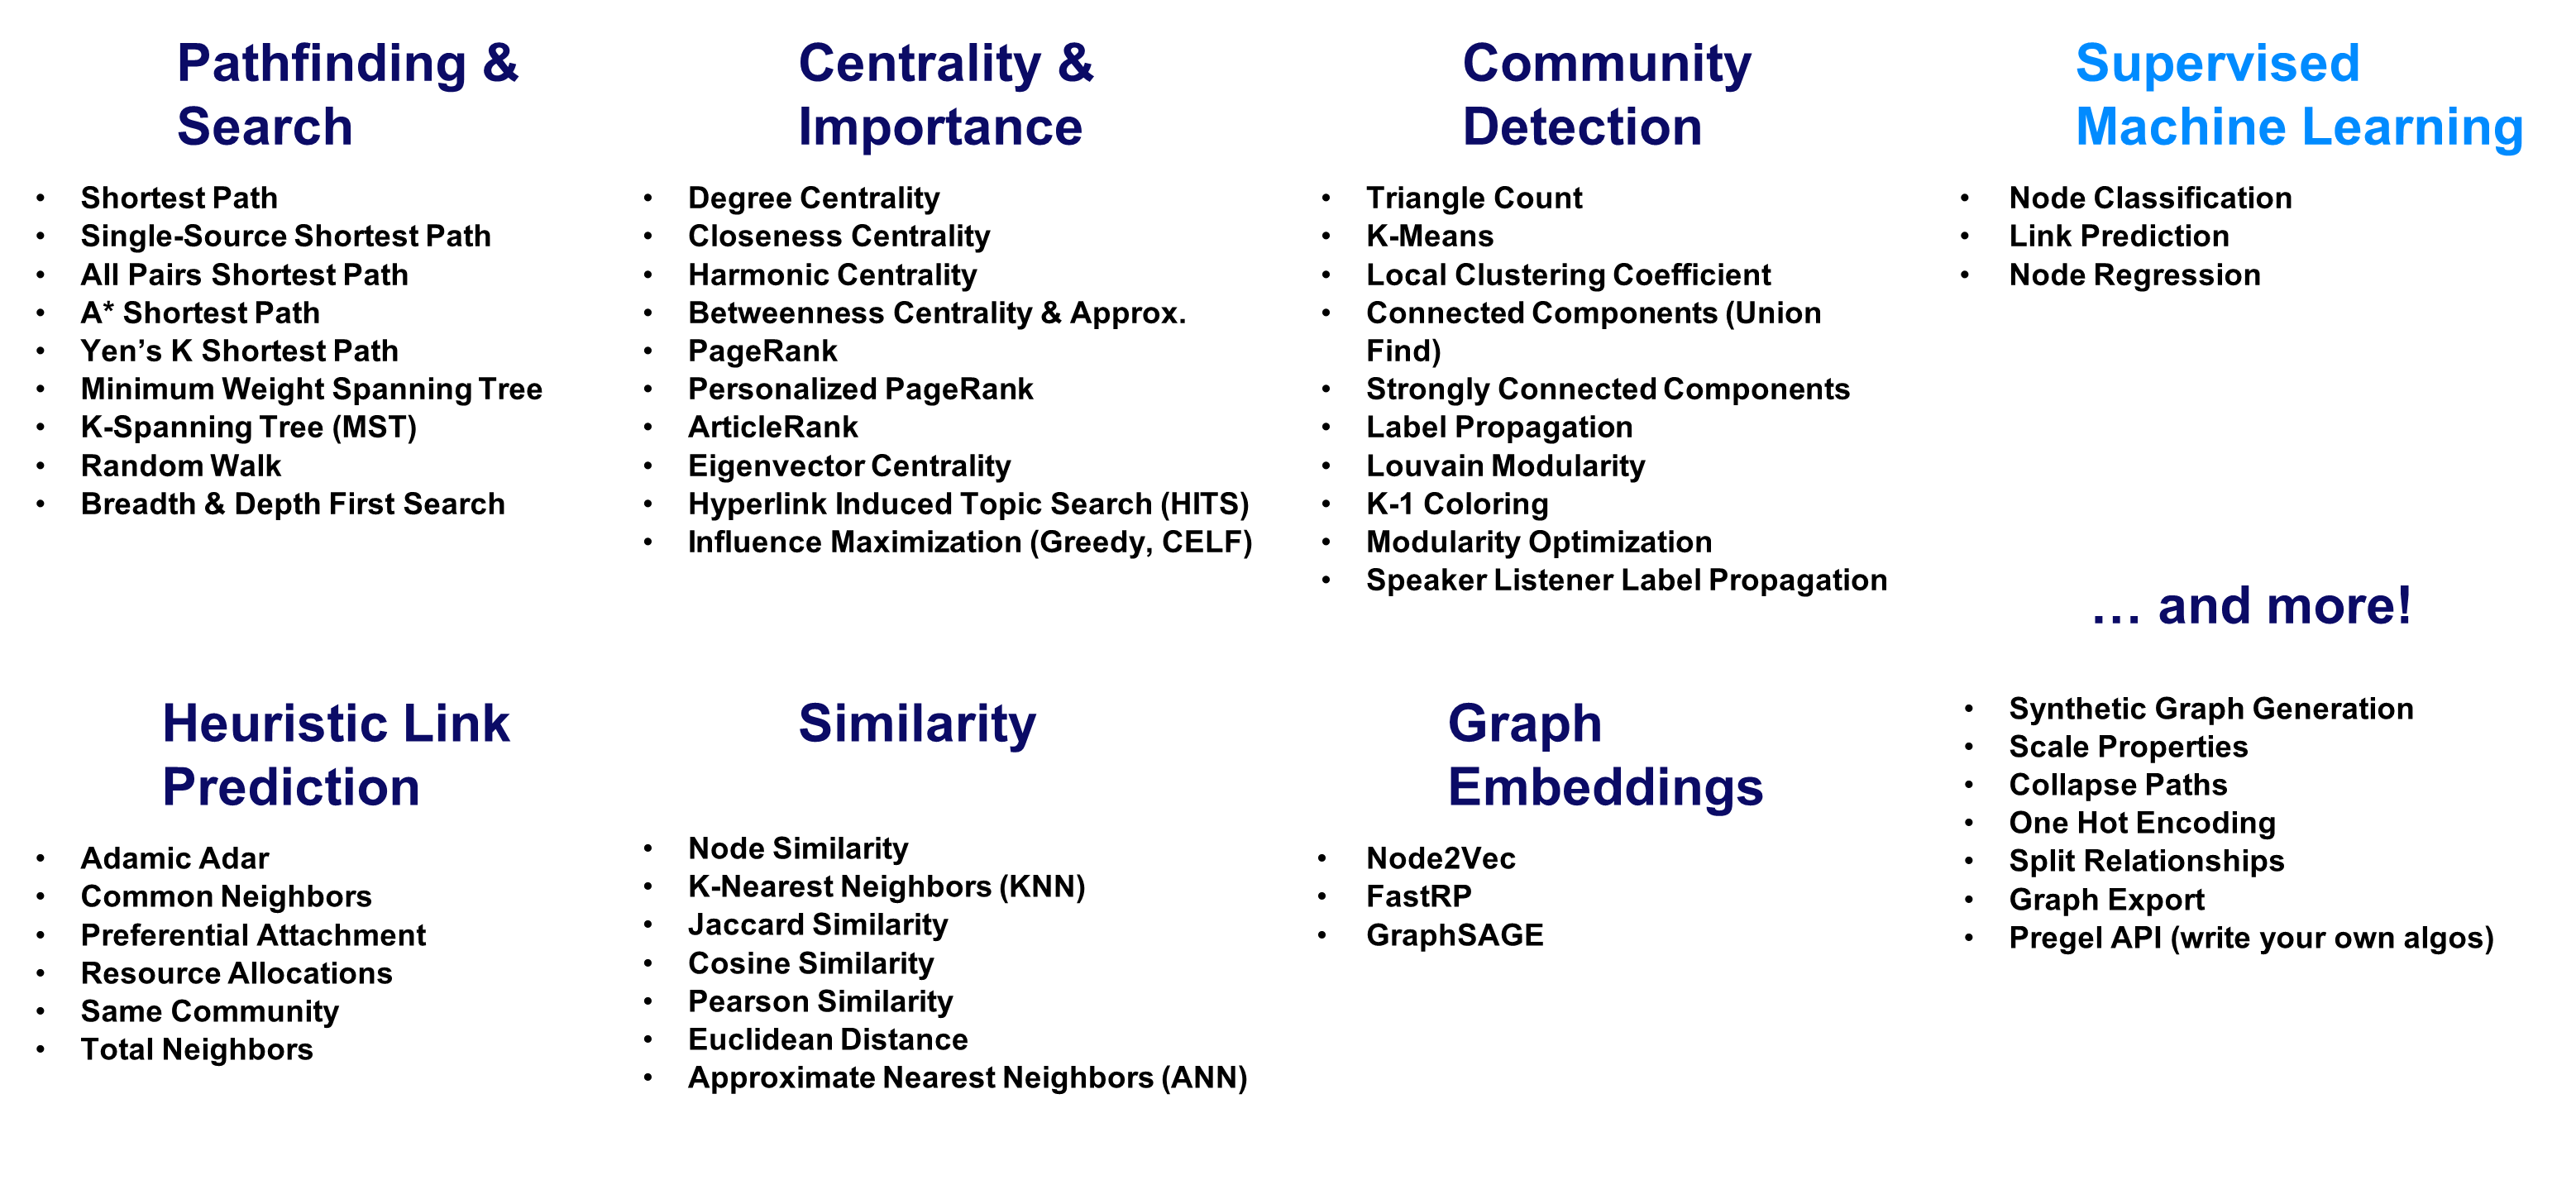
\includegraphics[width=\linewidth,keepaspectratio]{gds16}
\end{center}

\end{frame}


%%%%%%%%%%%%%%%%%%%%%%%%%%%%%%%%%%%%%%%%%%%%%%%%%%%%%%%%%%%%%%%%%%%%%%%%%%%%%%%%%%
\begin{frame}[fragile]\frametitle{What are Graph Algorithms?}

\begin{center}
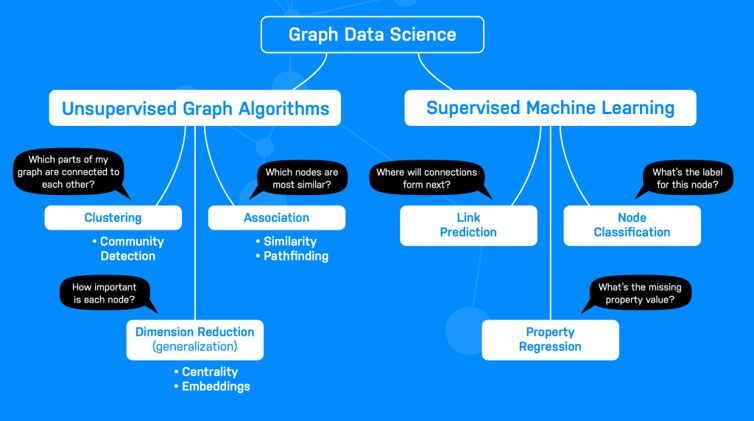
\includegraphics[width=\linewidth,keepaspectratio]{gds17}
\end{center}

\end{frame}


%%%%%%%%%%%%%%%%%%%%%%%%%%%%%%%%%%%%%%%%%%%%%%%%%%%%%%%%%%%%%%%%%%%%%%%%%%%%%%%%%%
\begin{frame}[fragile]\frametitle{Enriched Knowledge Graphs}

\begin{center}
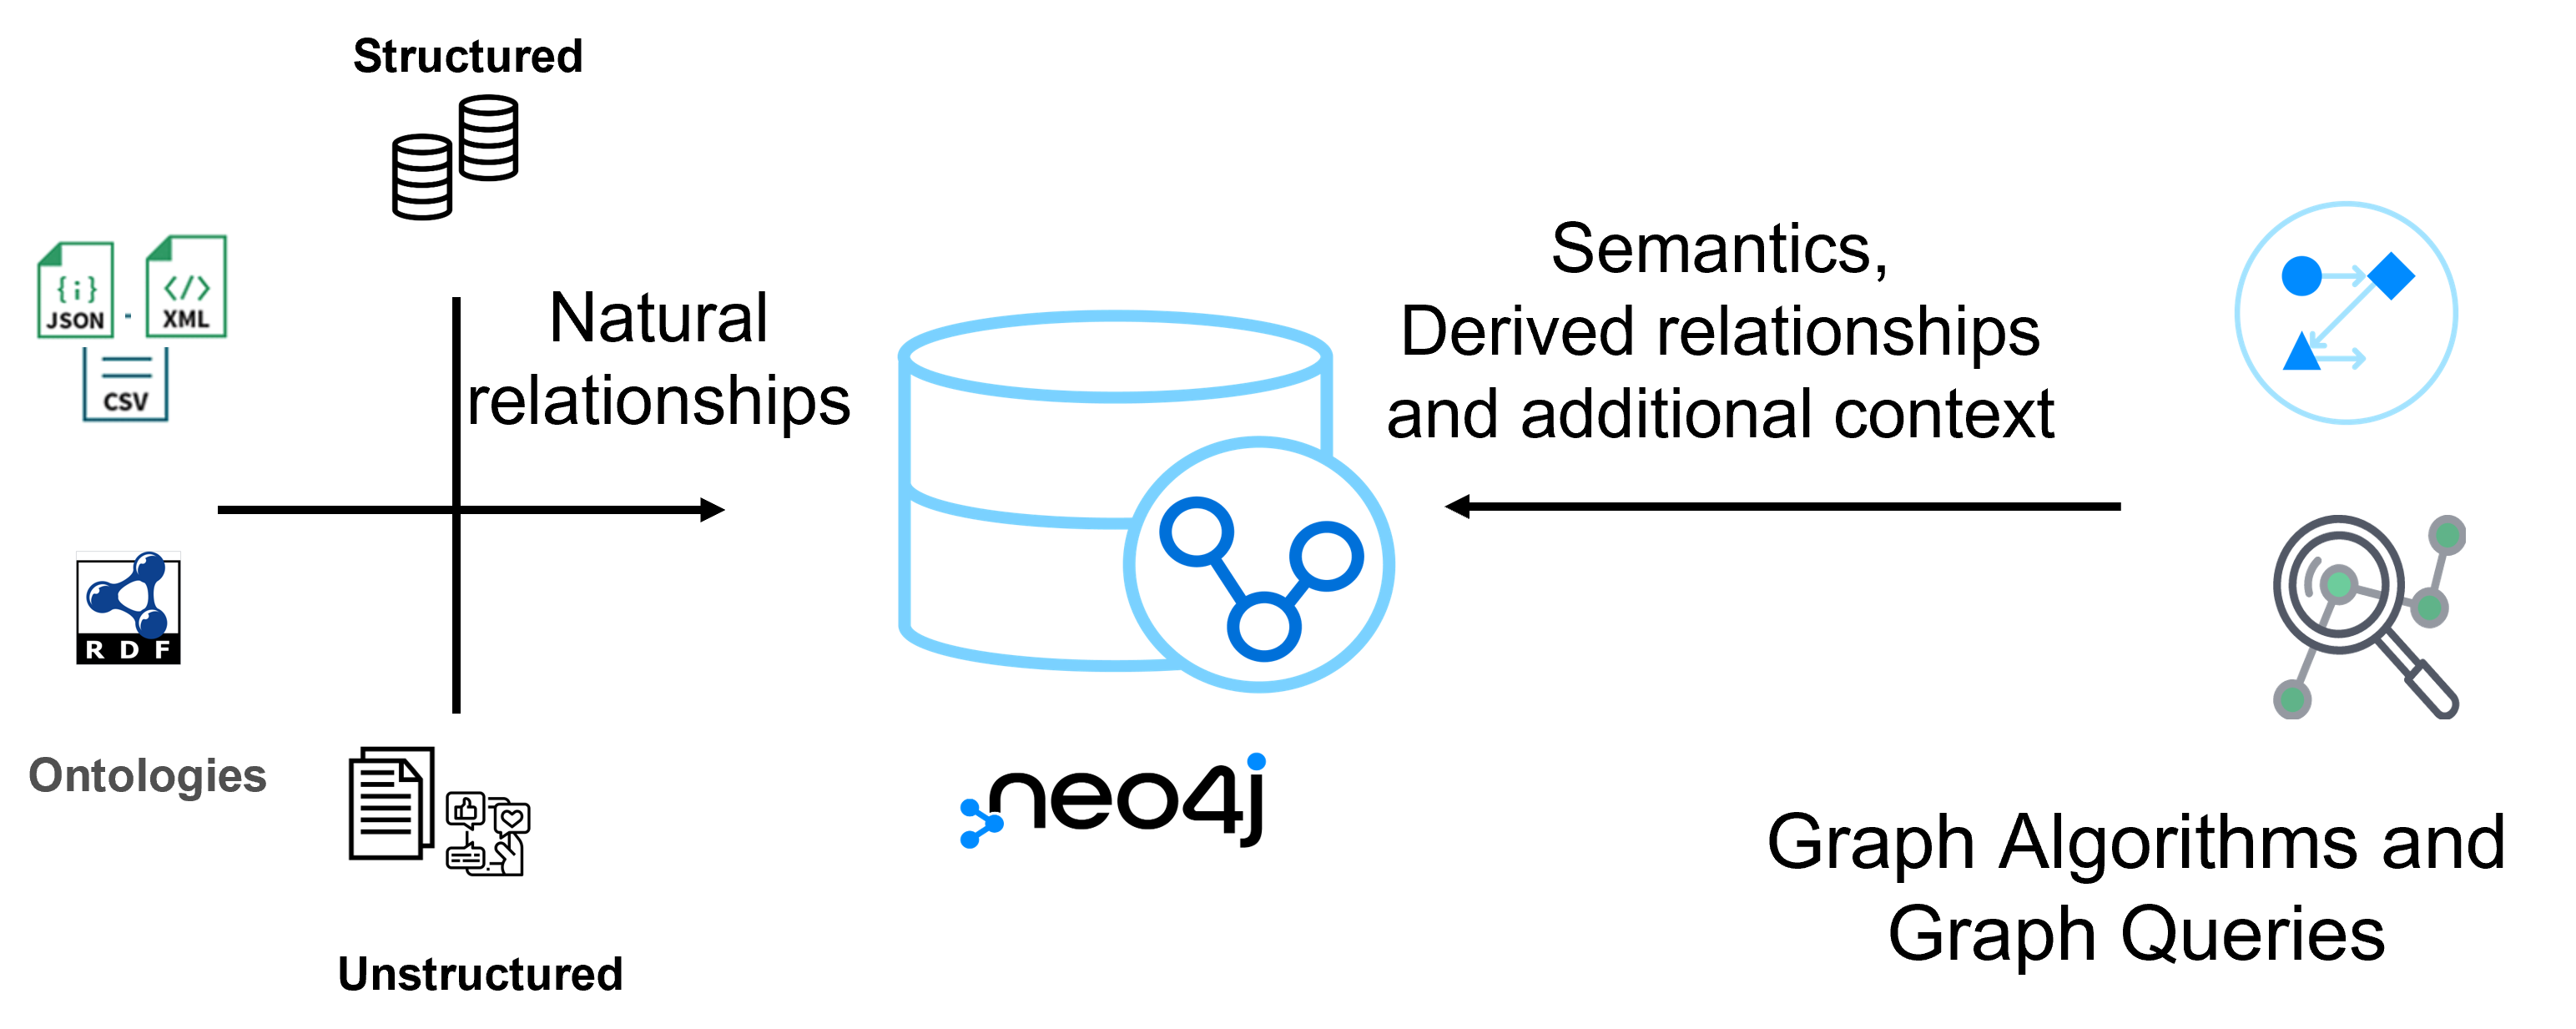
\includegraphics[width=\linewidth,keepaspectratio]{gds18}
\end{center}

\end{frame}


%%%%%%%%%%%%%%%%%%%%%%%%%%%%%%%%%%%%%%%%%%%%%%%%%%%%%%%%%%%%%%%%%%%%%%%%%%%%%%%%%%
\begin{frame}[fragile]\frametitle{Evolution of Graph Data Science}

\begin{center}
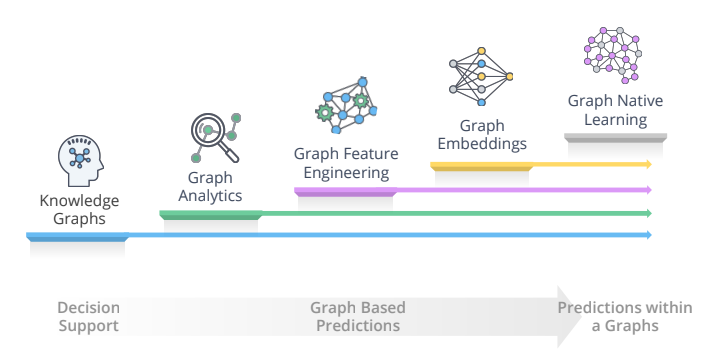
\includegraphics[width=\linewidth,keepaspectratio]{gds33}

{\tiny (Mark Needham - Intro to Graph Data Science with Neo4j)}

\end{center}

\end{frame}


%%%%%%%%%%%%%%%%%%%%%%%%%%%%%%%%%%%%%%%%%%%%%%%%%%%%%%%%%%%%%%%%%%%%%%%%%%%%%%%%%%
\begin{frame}[fragile]\frametitle{Identity Management / Entity Resolution}

Graph algorithms and graph embeddings are used for generating context and resolving identities/entities


\begin{center}
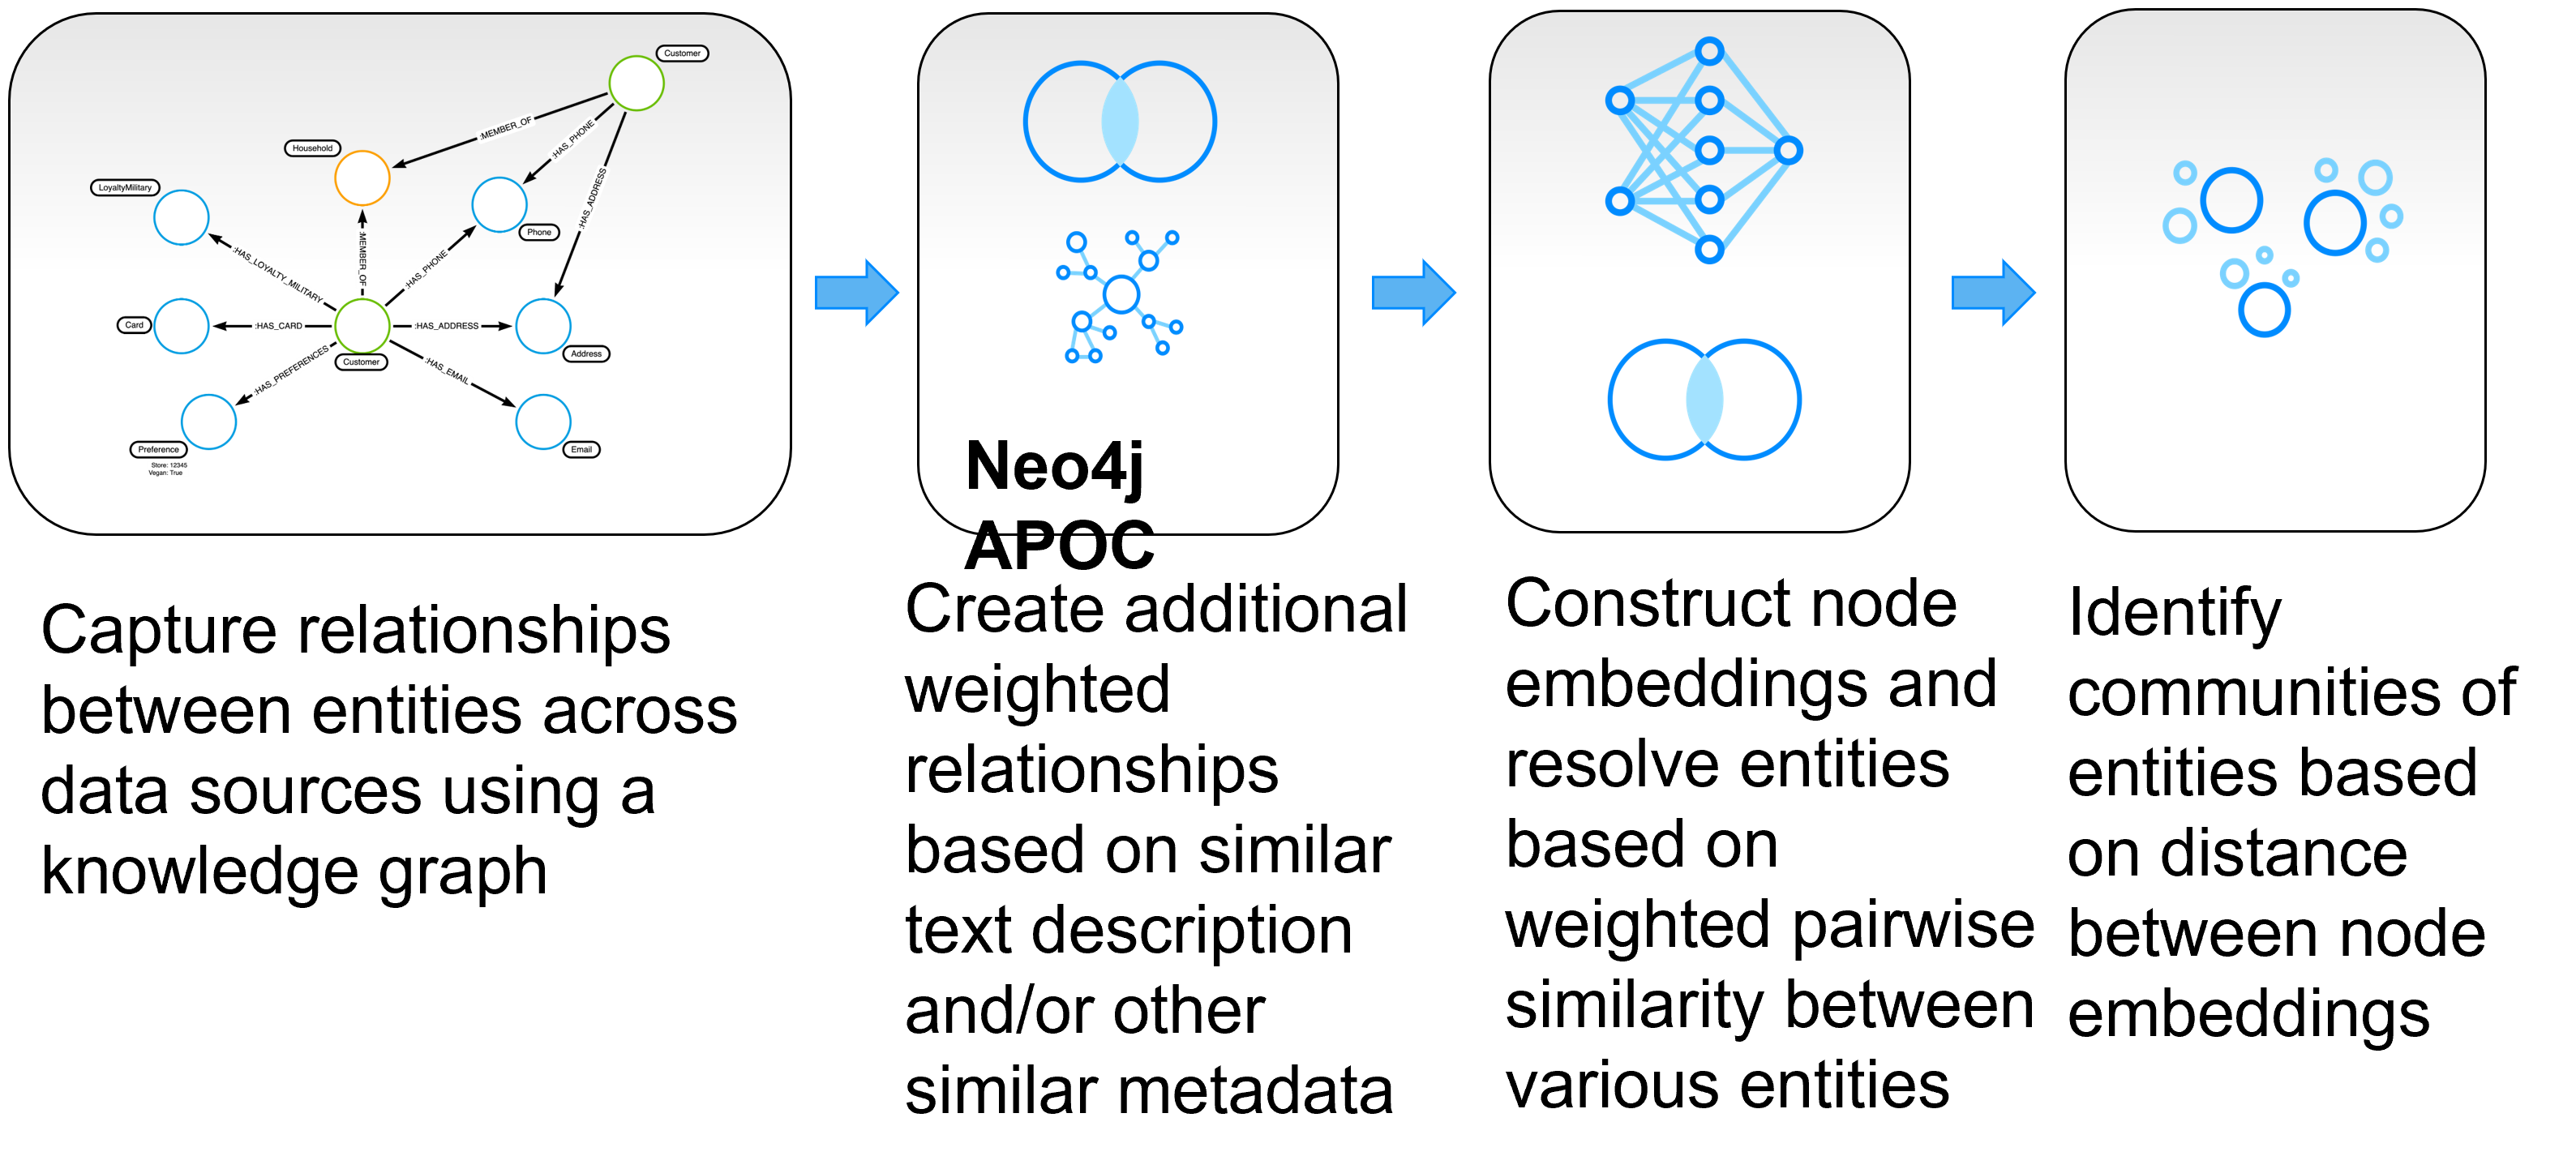
\includegraphics[width=\linewidth,keepaspectratio]{gds19}
\end{center}

\end{frame}

%%%%%%%%%%%%%%%%%%%%%%%%%%%%%%%%%%%%%%%%%%%%%%%%%%%%%%%%%%%%%%%%%%%%%%%%%%%%%%%%%%
\begin{frame}[fragile]\frametitle{Personalized Recommendations}

Graph algorithms and graph embeddings are used for generating product recommendations and improving search relevance


\begin{center}
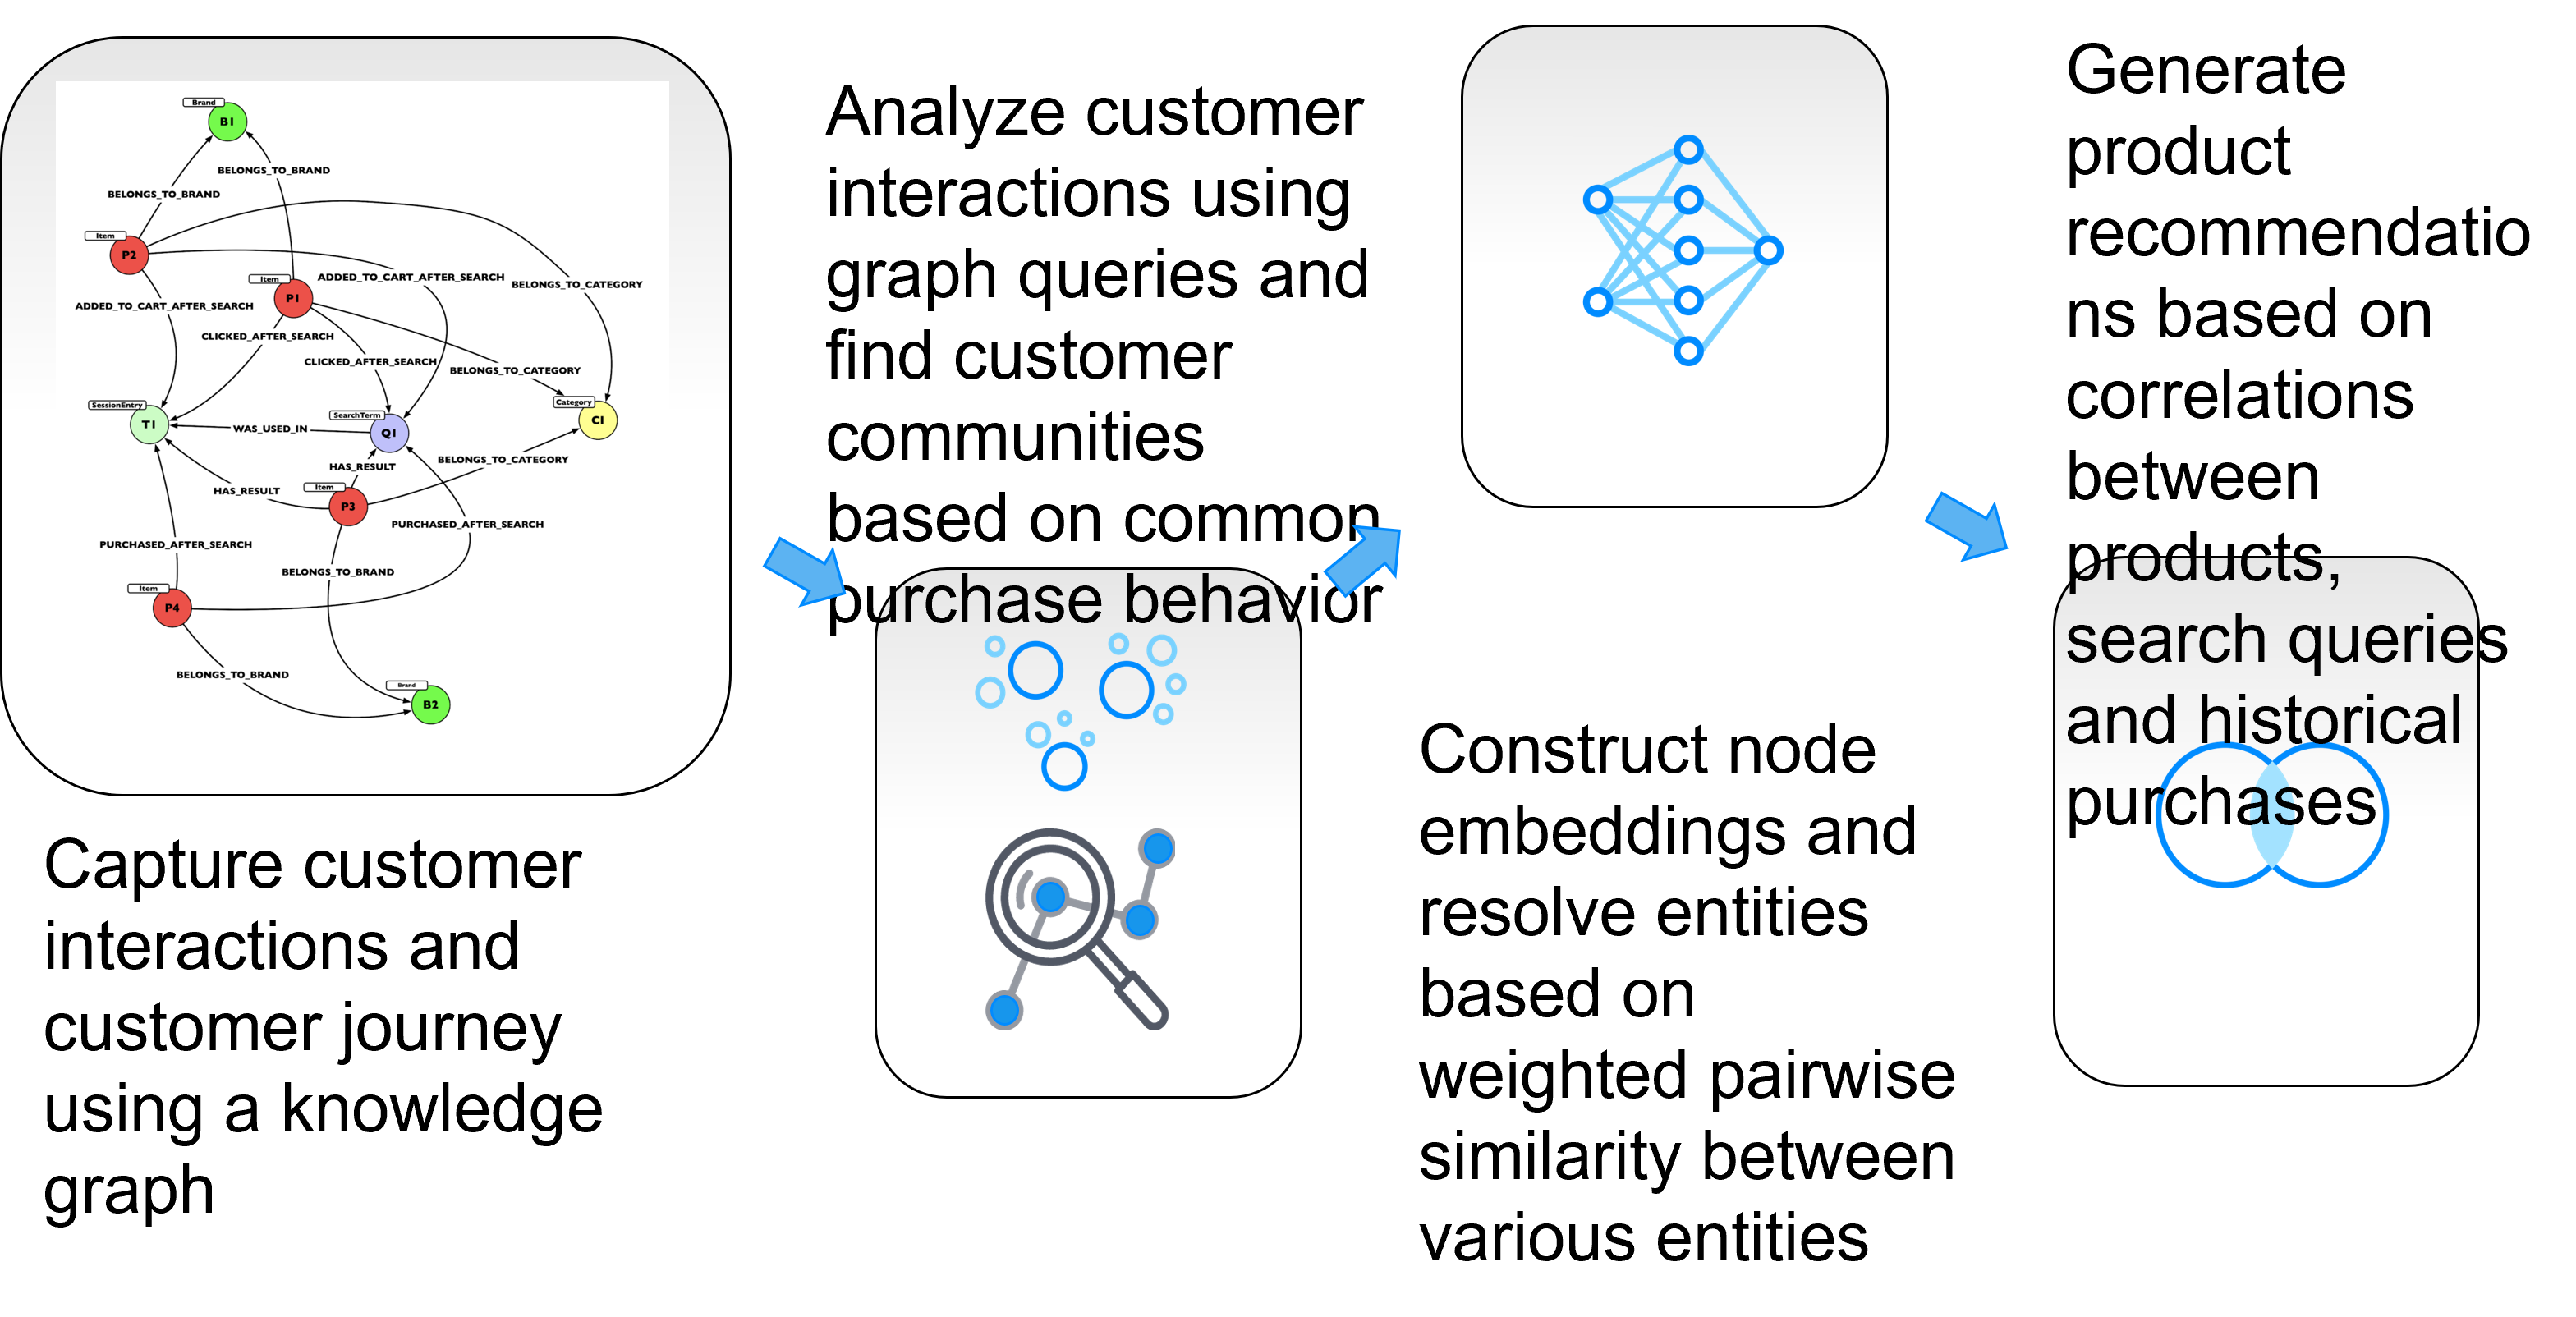
\includegraphics[width=\linewidth,keepaspectratio]{gds20}
\end{center}

\end{frame}

%%%%%%%%%%%%%%%%%%%%%%%%%%%%%%%%%%%%%%%%%%%%%%%%%%%%%%%%%%%%%%%%%%%%%%%%%%%%%%%%%%
\begin{frame}[fragile]\frametitle{Life Sciences: Patient care}

Graphs and graph algorithms are used for capturing the events in patient journeys and analyze them for proactive monitoring


\begin{center}
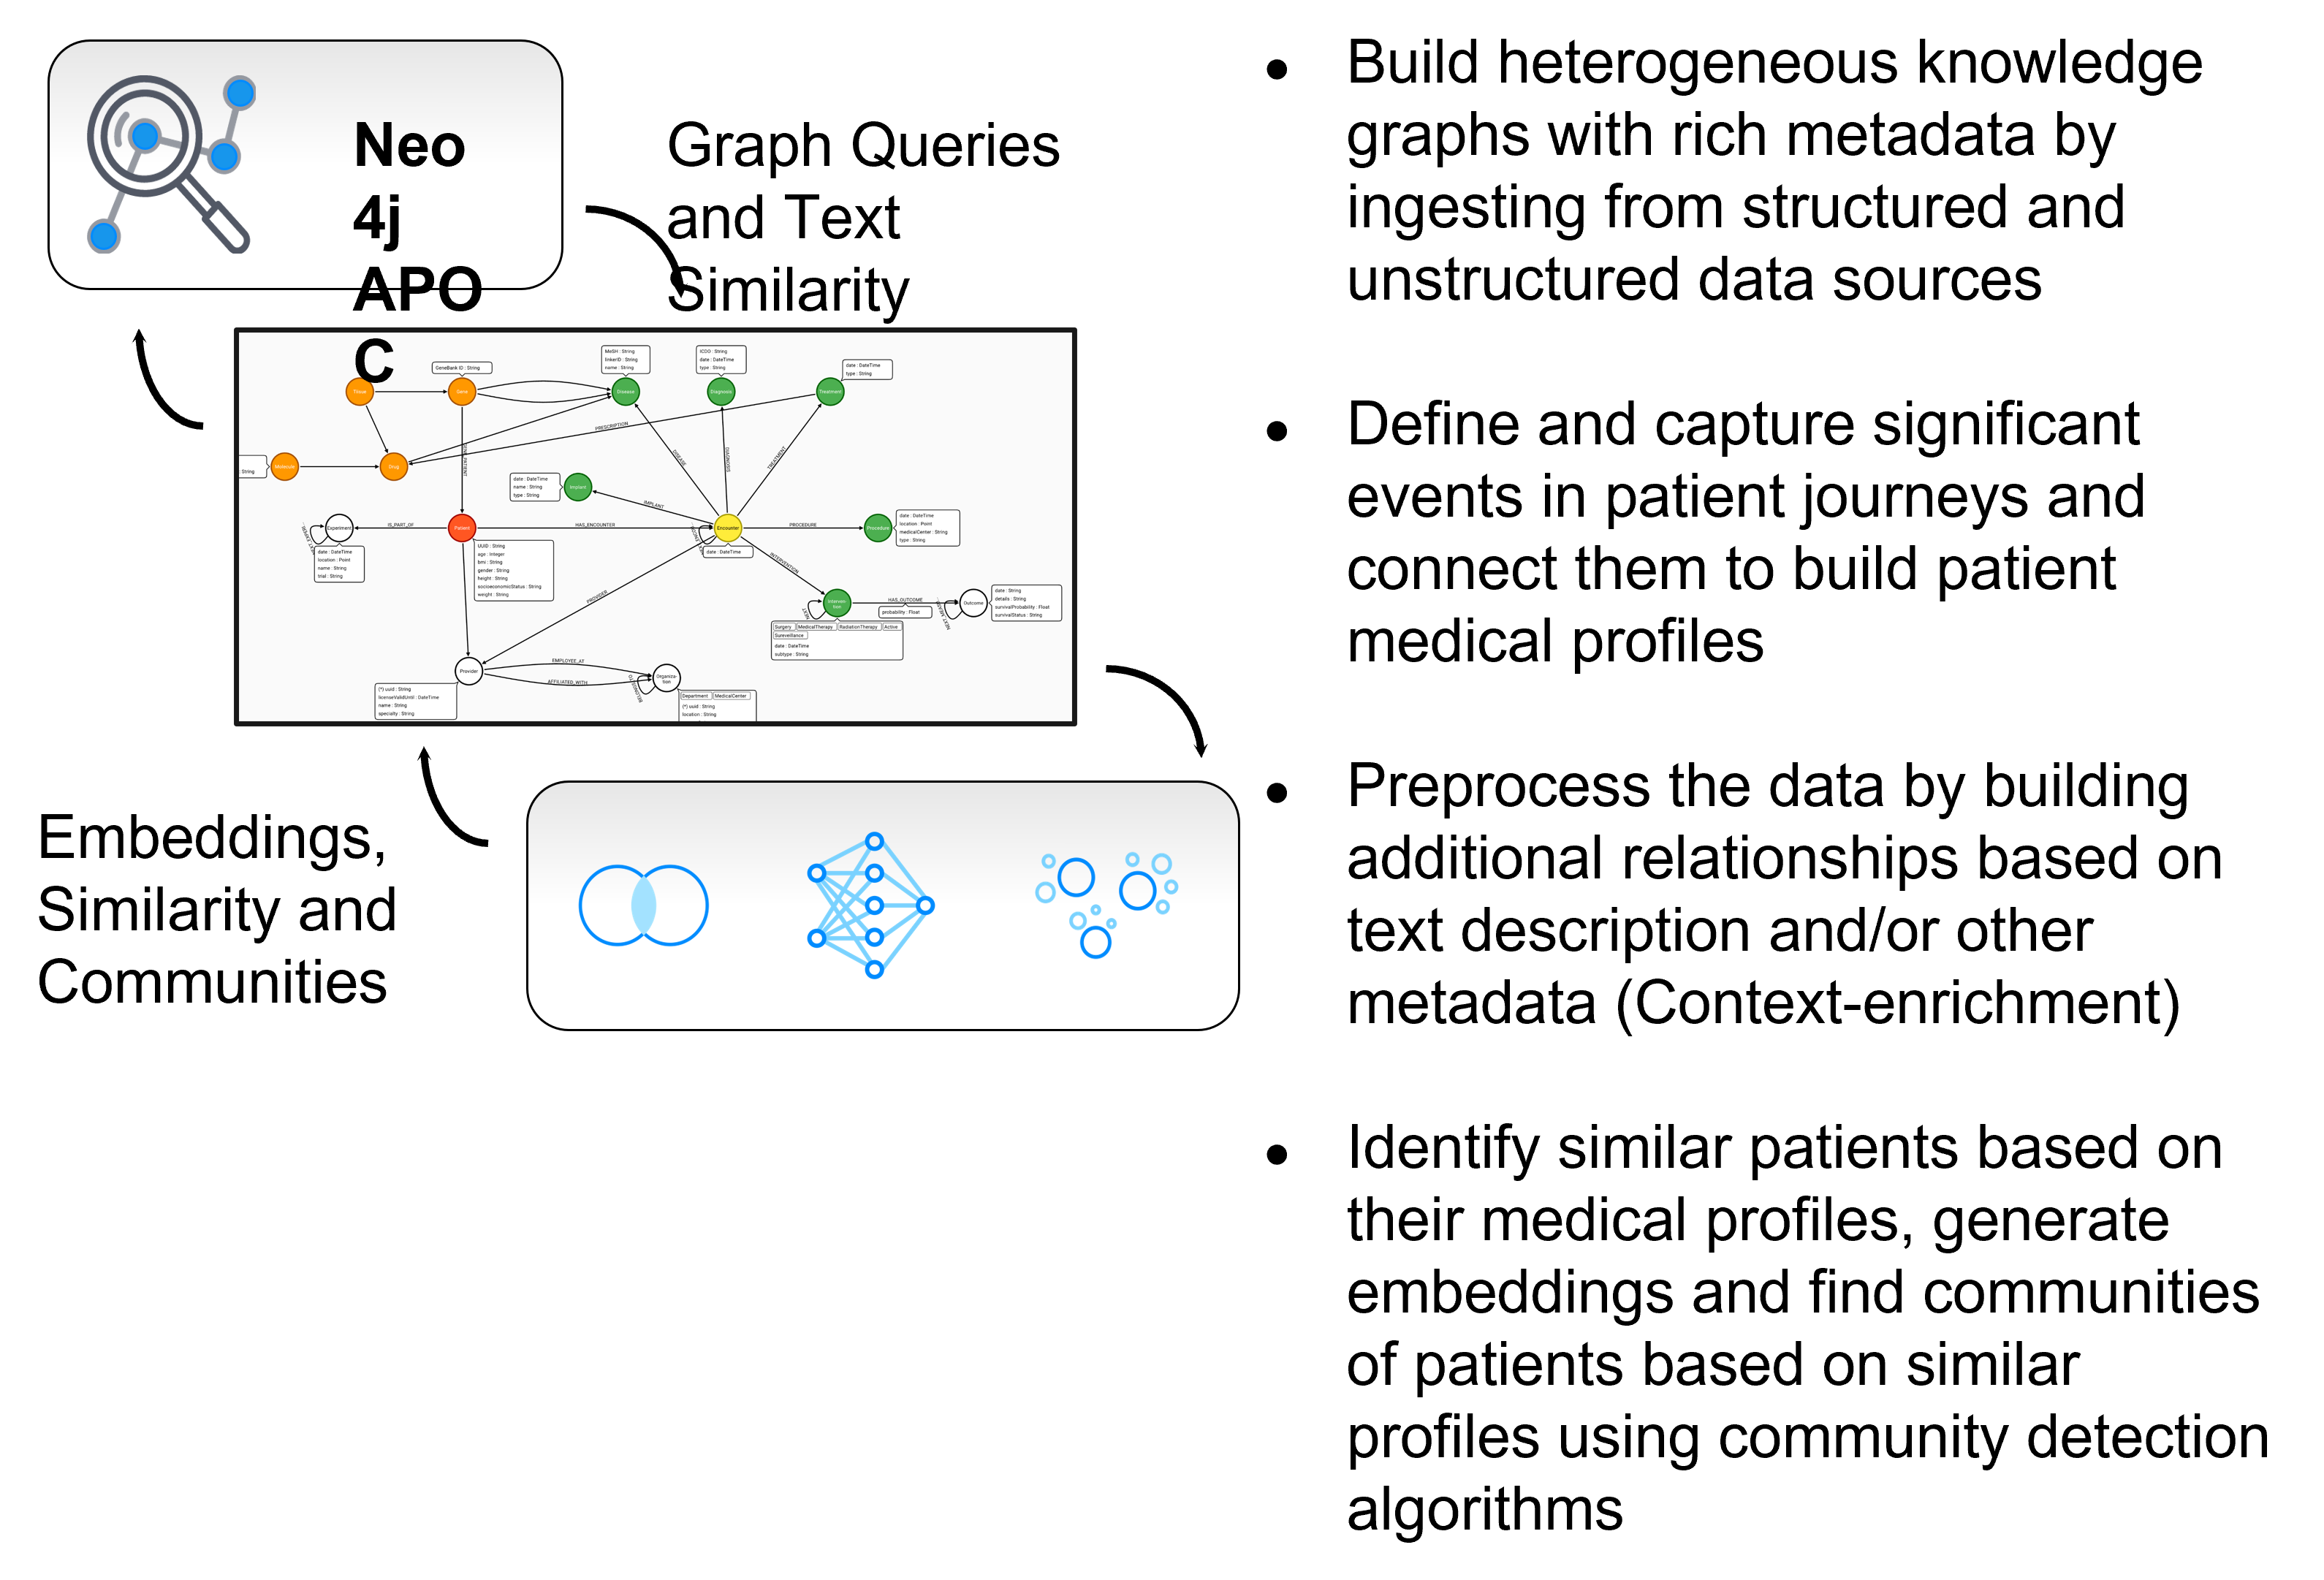
\includegraphics[width=0.9\linewidth,keepaspectratio]{gds21}
\end{center}

\end{frame}

%%%%%%%%%%%%%%%%%%%%%%%%%%%%%%%%%%%%%%%%%%%%%%%%%%%%%%%%%%%%%%%%%%%%%%%%%%%%%%%%%%
\begin{frame}[fragile]\frametitle{Graph Data Science}

\begin{center}
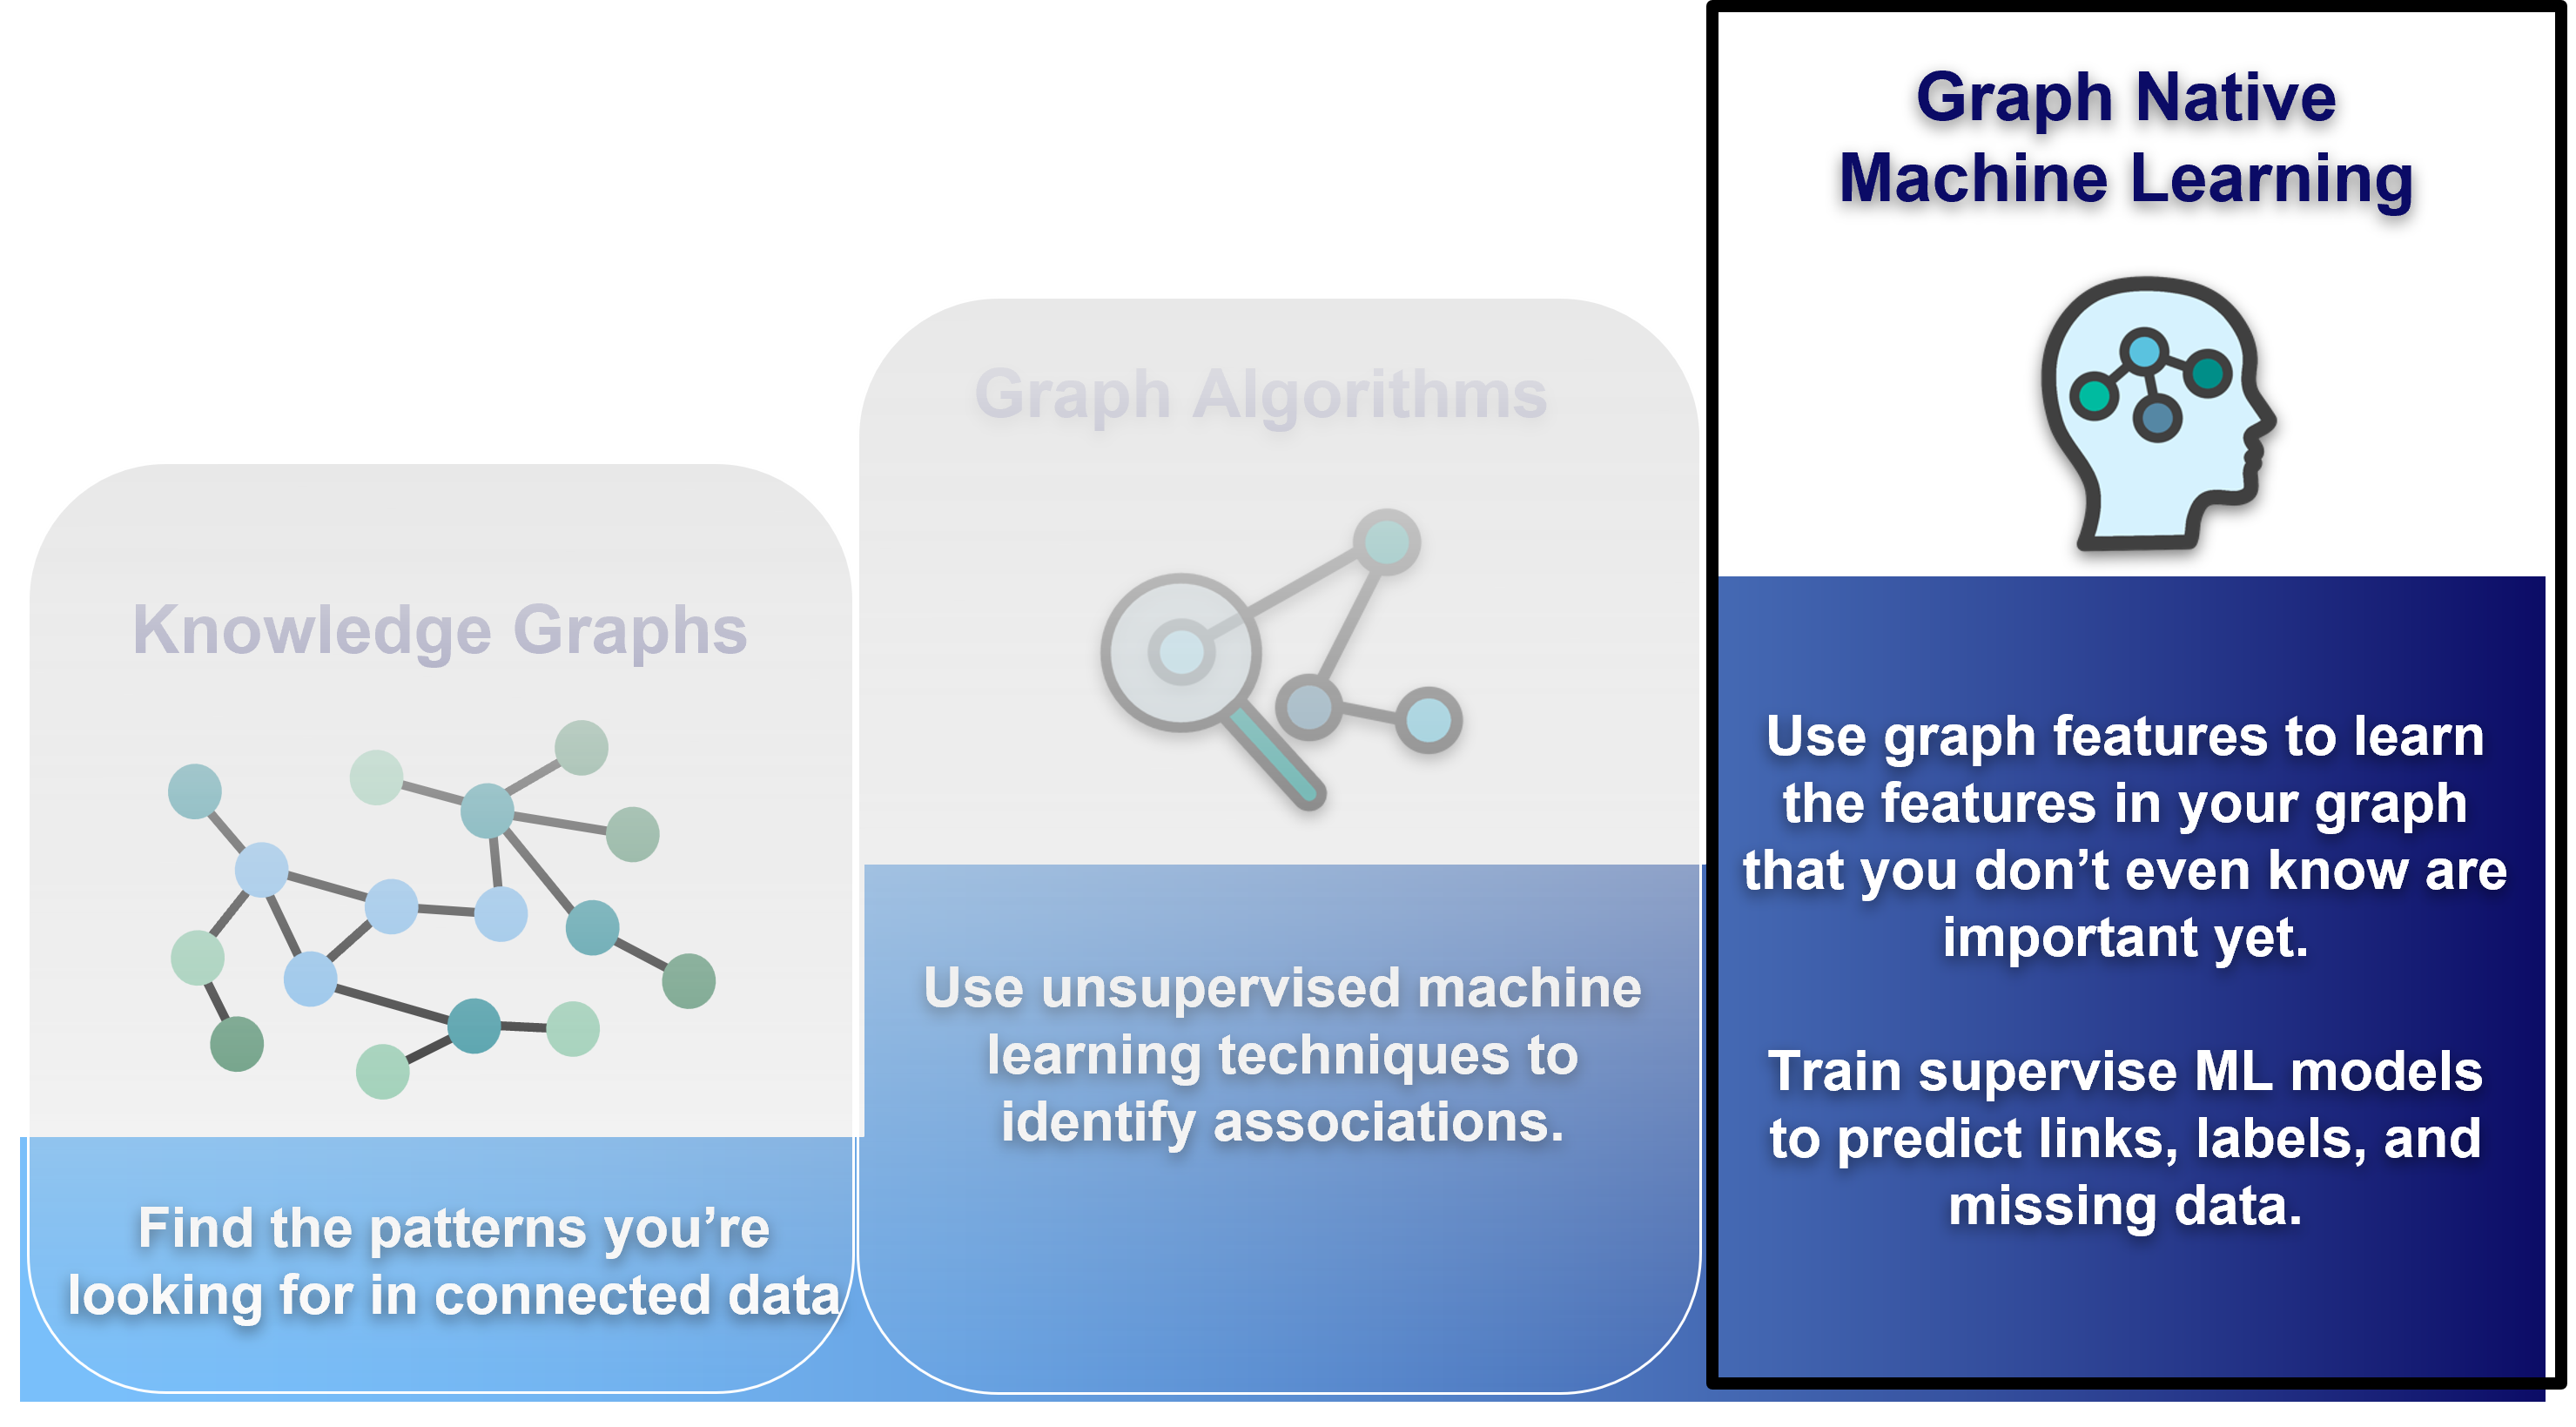
\includegraphics[width=\linewidth,keepaspectratio]{gds22}
\end{center}

\end{frame}

%%%%%%%%%%%%%%%%%%%%%%%%%%%%%%%%%%%%%%%%%%%%%%%%%%%%%%%%%%%%%%%%%%%%%%%%%%%%%%%%%%
\begin{frame}[fragile]\frametitle{Relationship-Driven AI}

\begin{itemize}
\item Traditional ML ignore network structure because it’s difficult to extract
\item Use the right data structures to store and retrieve relationships 
\item Add relationships to AI/ML pipelines to make them contextual and to unlock otherwise unattainable predictions
\end{itemize}

\begin{center}
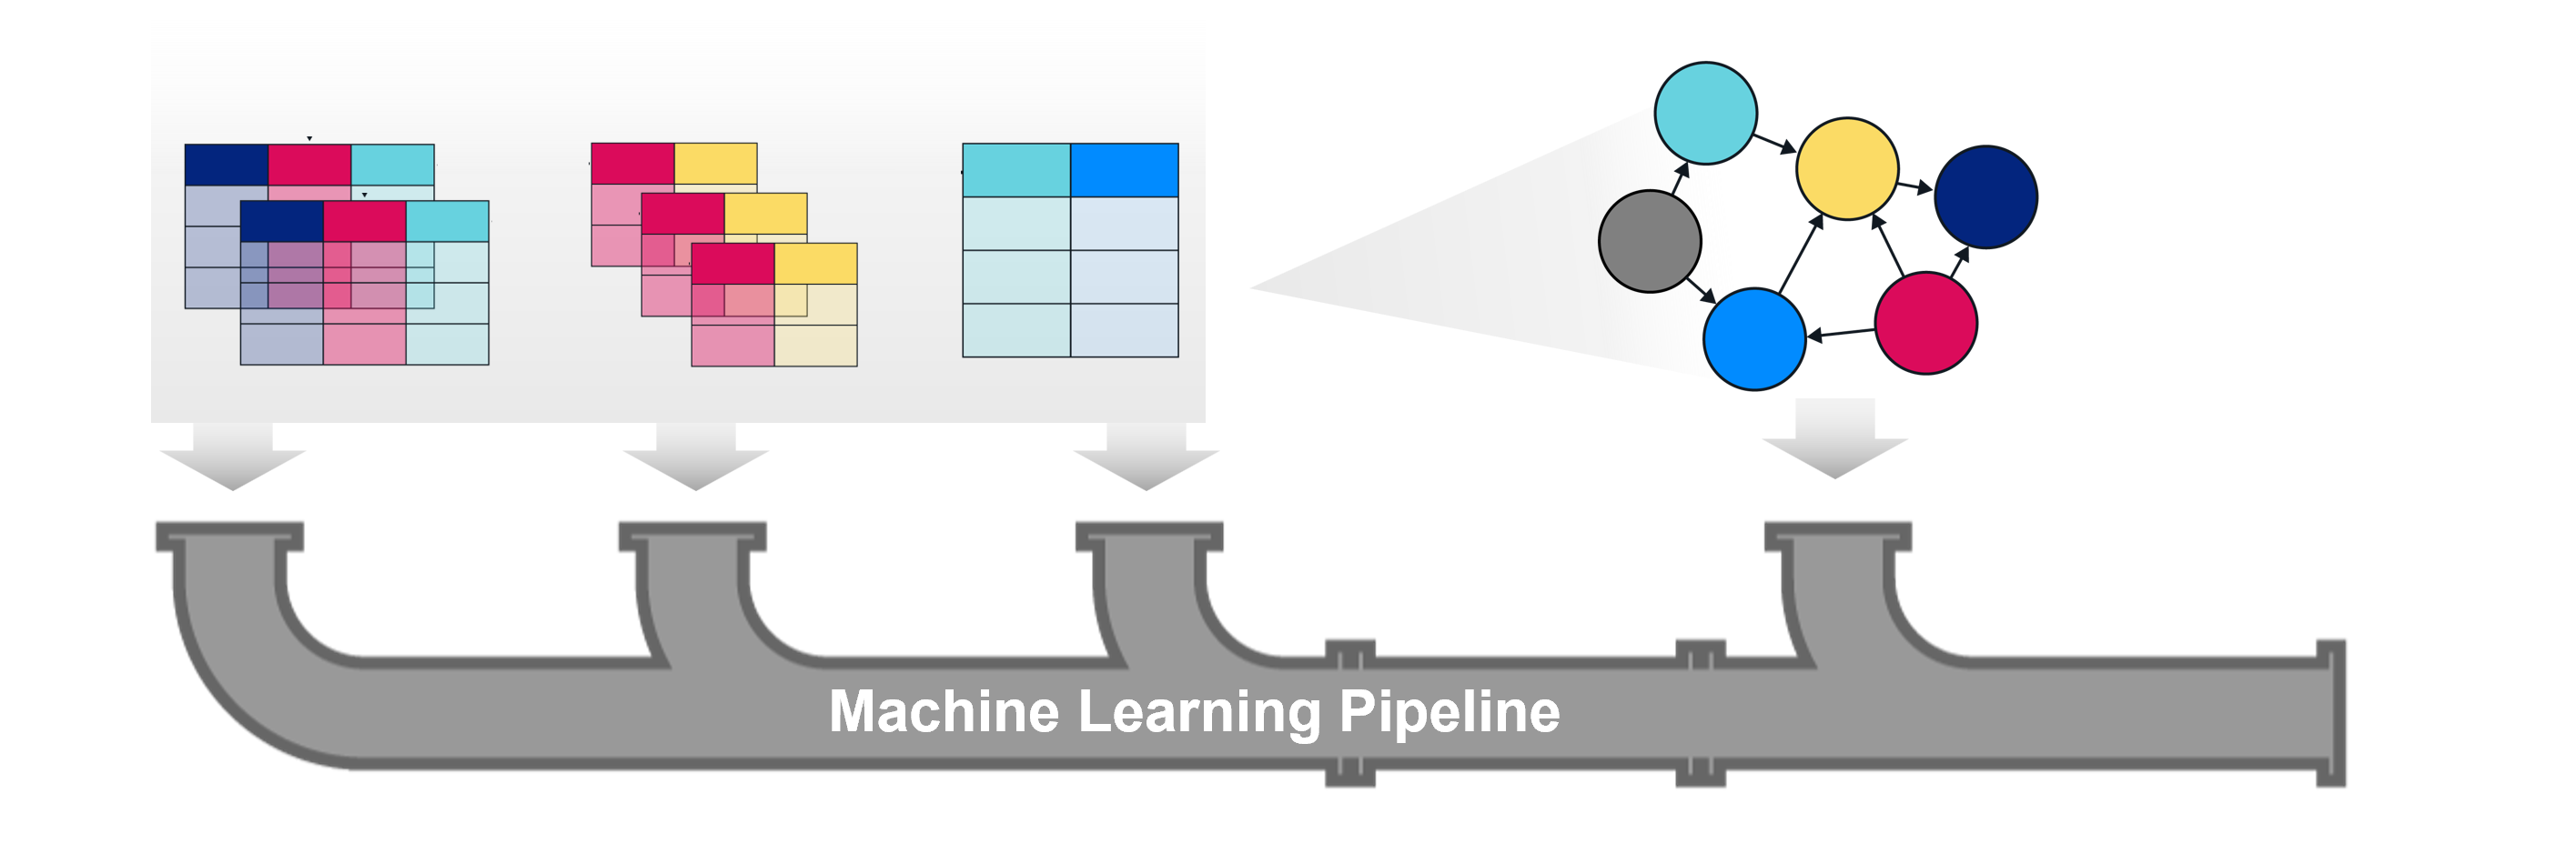
\includegraphics[width=\linewidth,keepaspectratio]{gds23}
\end{center}

\end{frame}


%%%%%%%%%%%%%%%%%%%%%%%%%%%%%%%%%%%%%%%%%%%%%%%%%%%%%%%%%%%%%%%%%%%%%%%%%%%%%%%%%%
\begin{frame}[fragile]\frametitle{Graph Feature Engineering}

\begin{center}
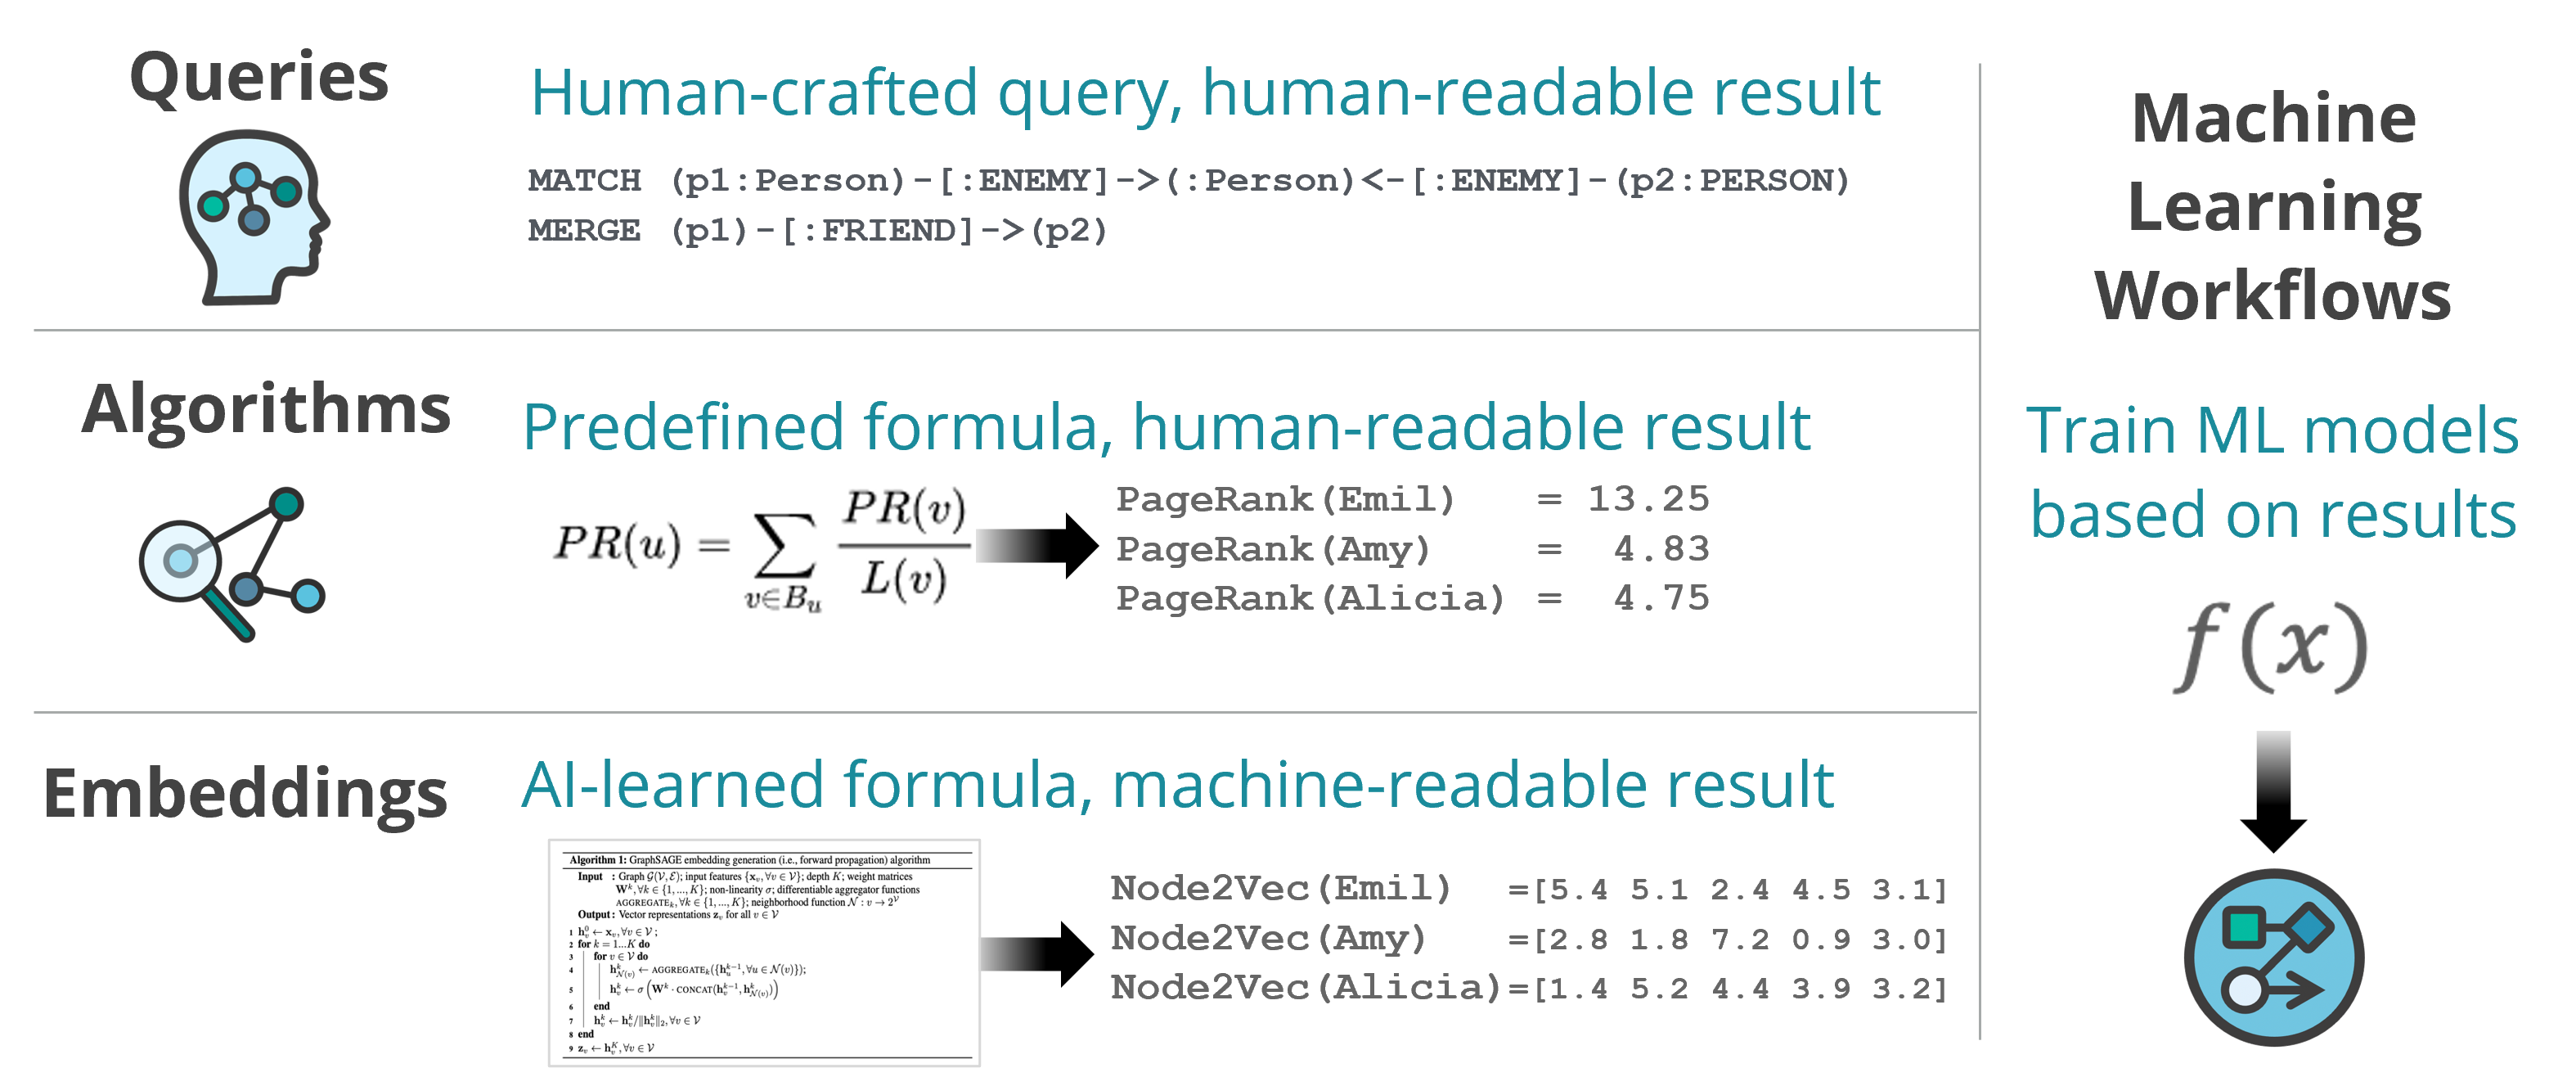
\includegraphics[width=\linewidth,keepaspectratio]{gds24}
\end{center}

\end{frame}


%%%%%%%%%%%%%%%%%%%%%%%%%%%%%%%%%%%%%%%%%%%%%%%%%%%%%%%%%%%%%%%%%%%%%%%%%%%%%%%%%%
\begin{frame}[fragile]\frametitle{Graph Machine Learning}

\begin{center}
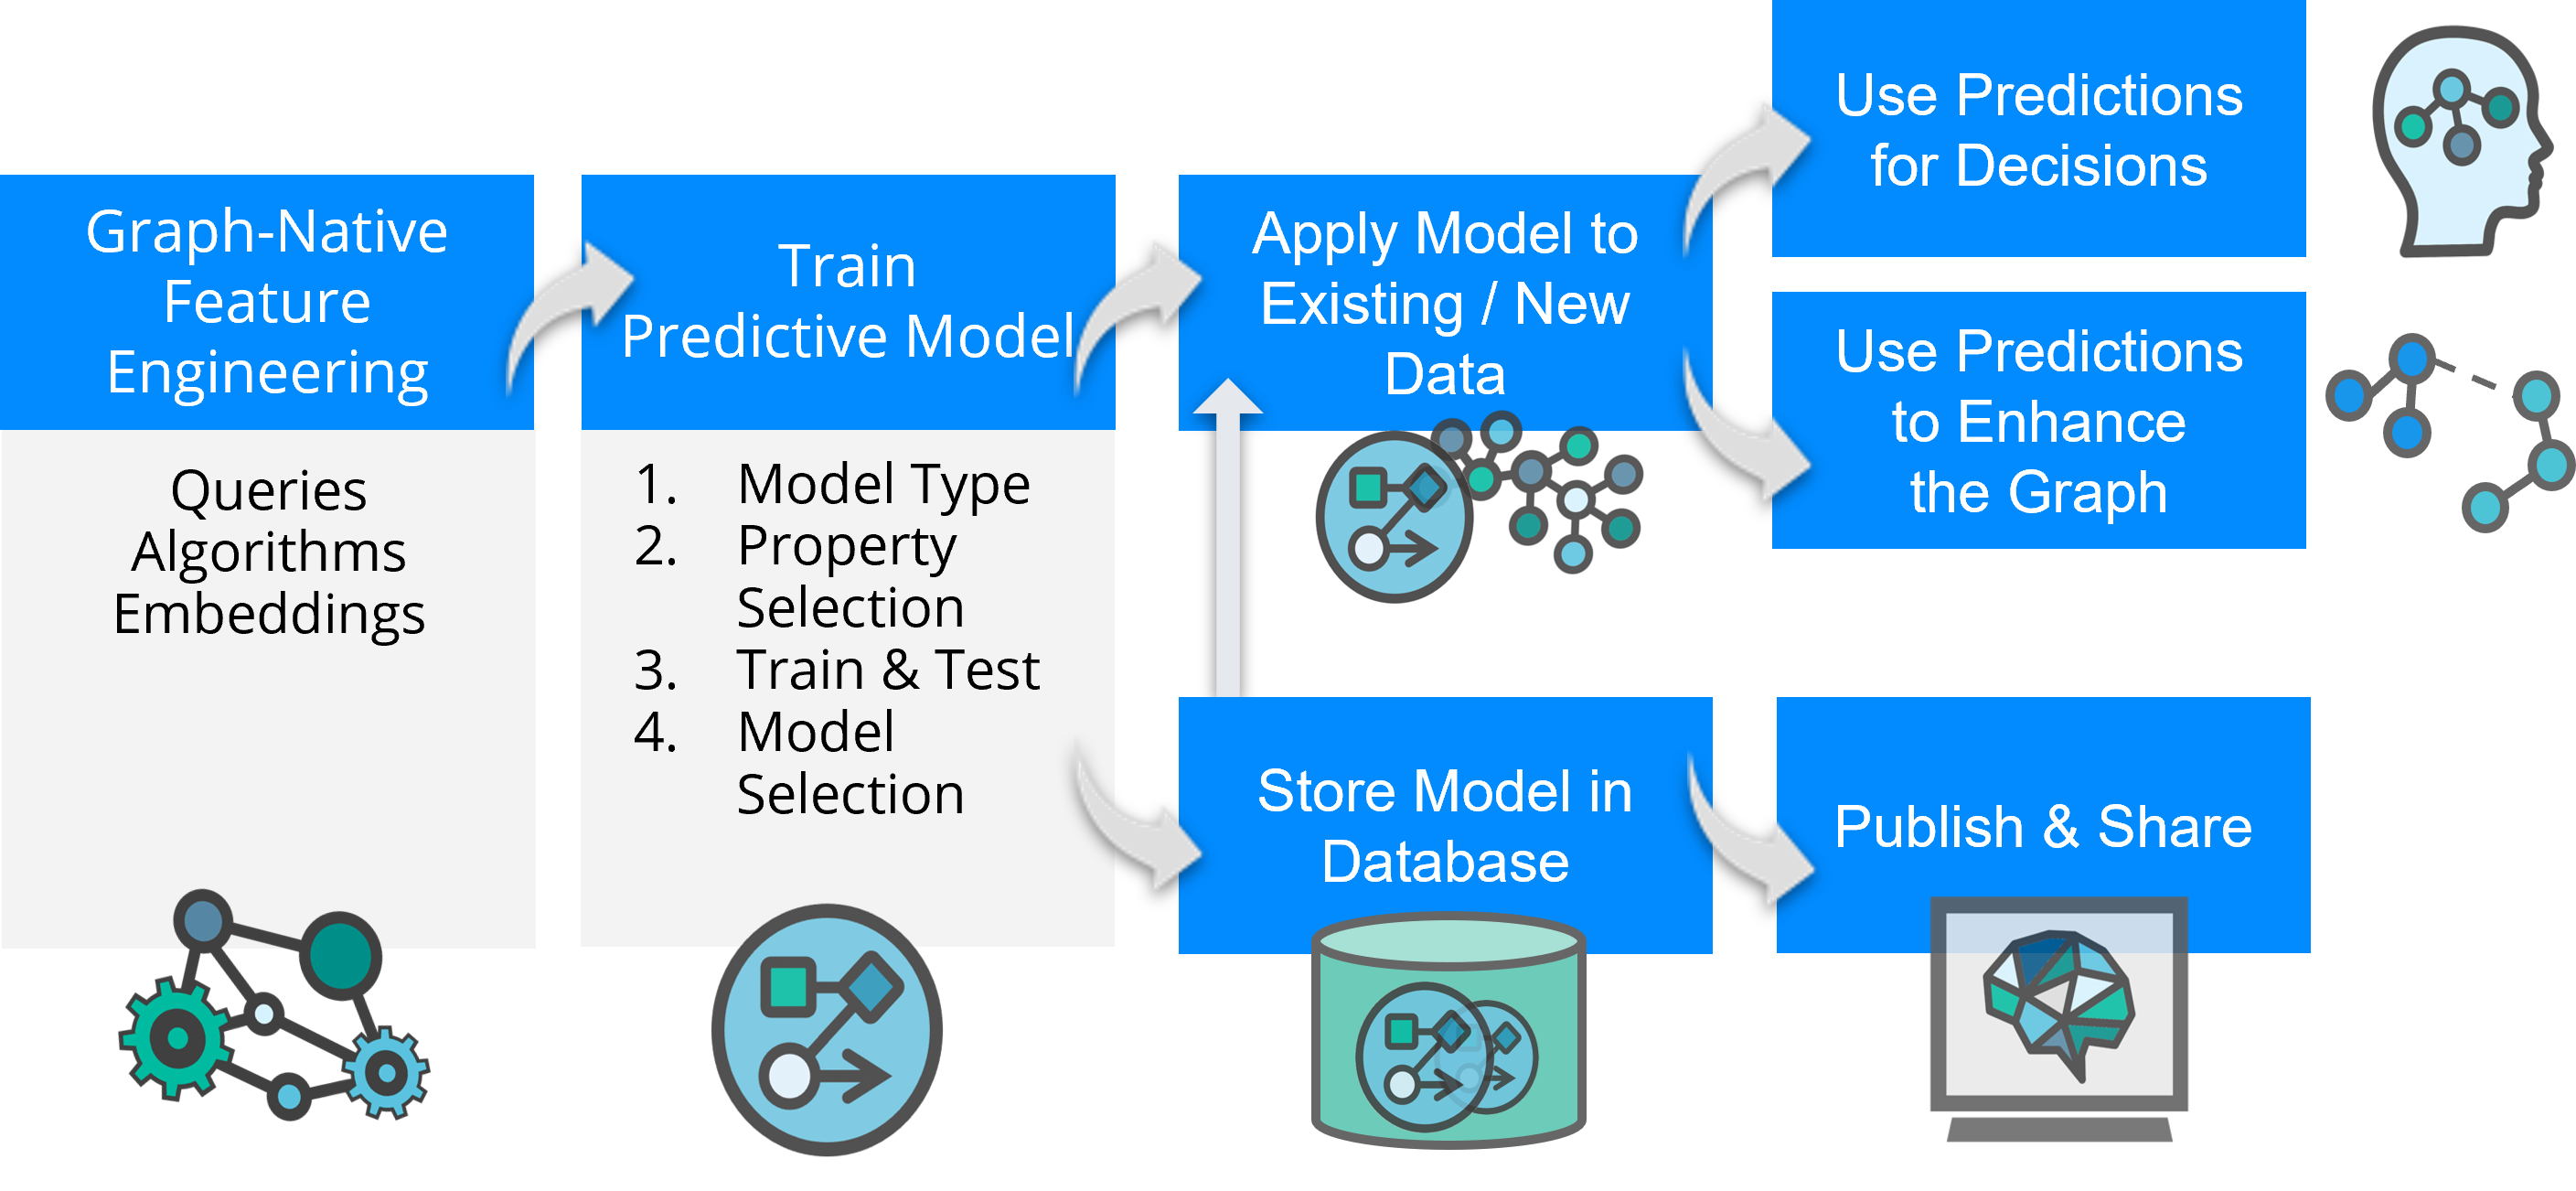
\includegraphics[width=\linewidth,keepaspectratio]{gds25}
\end{center}

The Only Completely In-Graph, ML Workflow

\end{frame}

%%%%%%%%%%%%%%%%%%%%%%%%%%%%%%%%%%%%%%%%%%%%%%%%%%%%%%%%%%%%%%%%%%%%%%%%%%%%%%%%%%
\begin{frame}[fragile]\frametitle{In-Graph Machine Learning}

\begin{center}
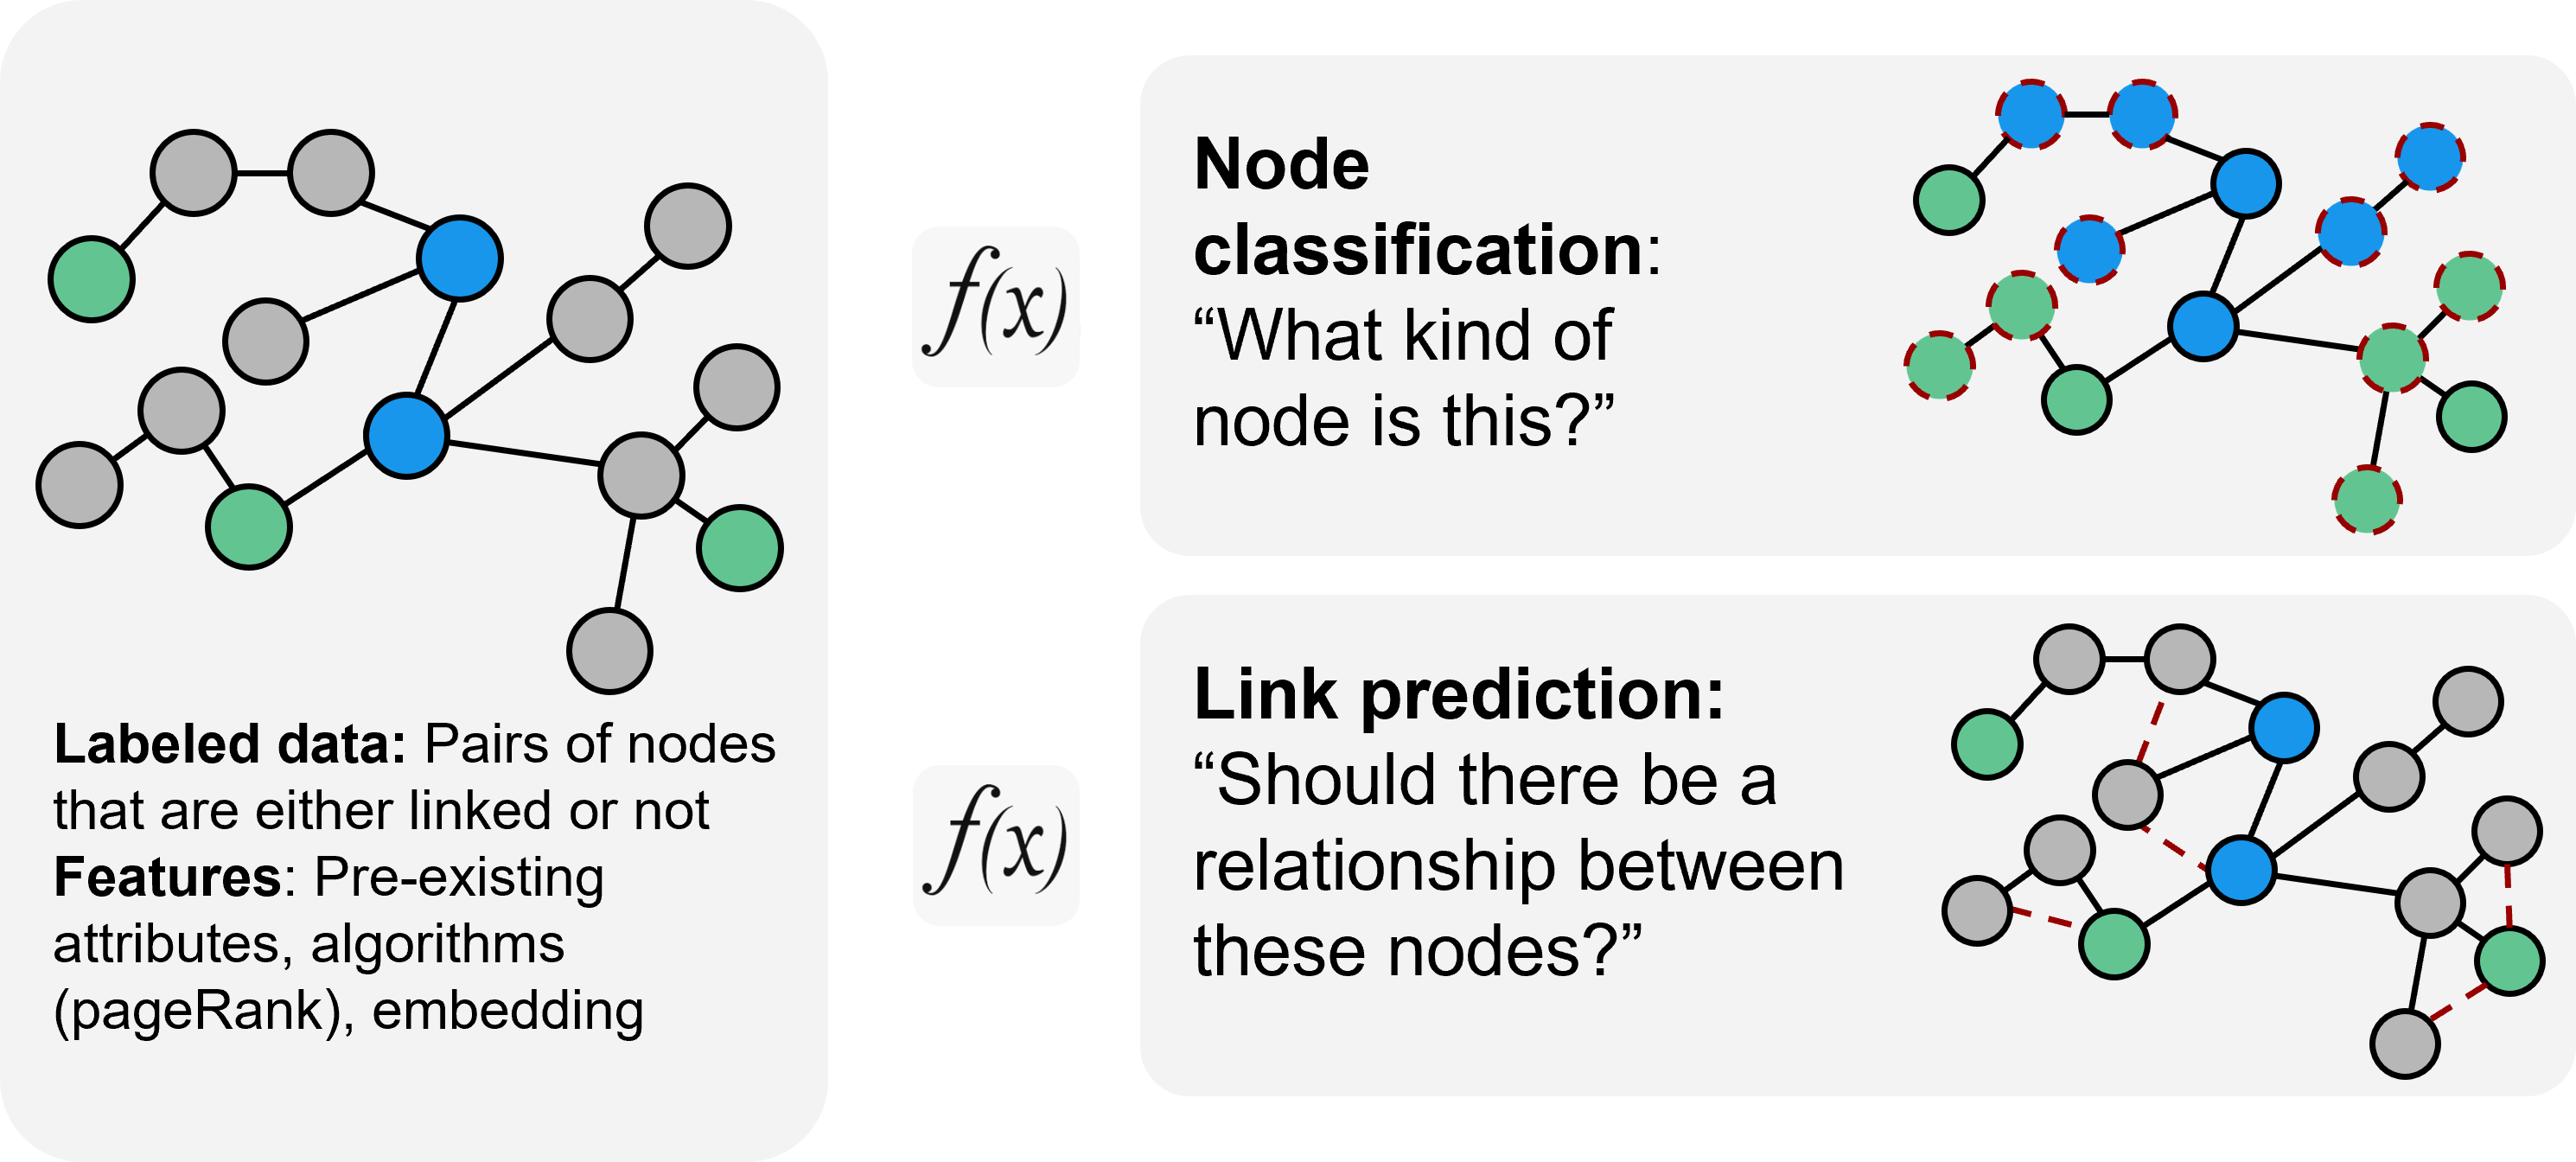
\includegraphics[width=\linewidth,keepaspectratio]{gds26}
\end{center}

\end{frame}

%%%%%%%%%%%%%%%%%%%%%%%%%%%%%%%%%%%%%%%%%%%%%%%%%%%%%%%%%%%%%%%%%%%%%%%%%%%%%%%%%%
\begin{frame}[fragile]\frametitle{Neo4j Graph Data Science Framework}

\begin{center}
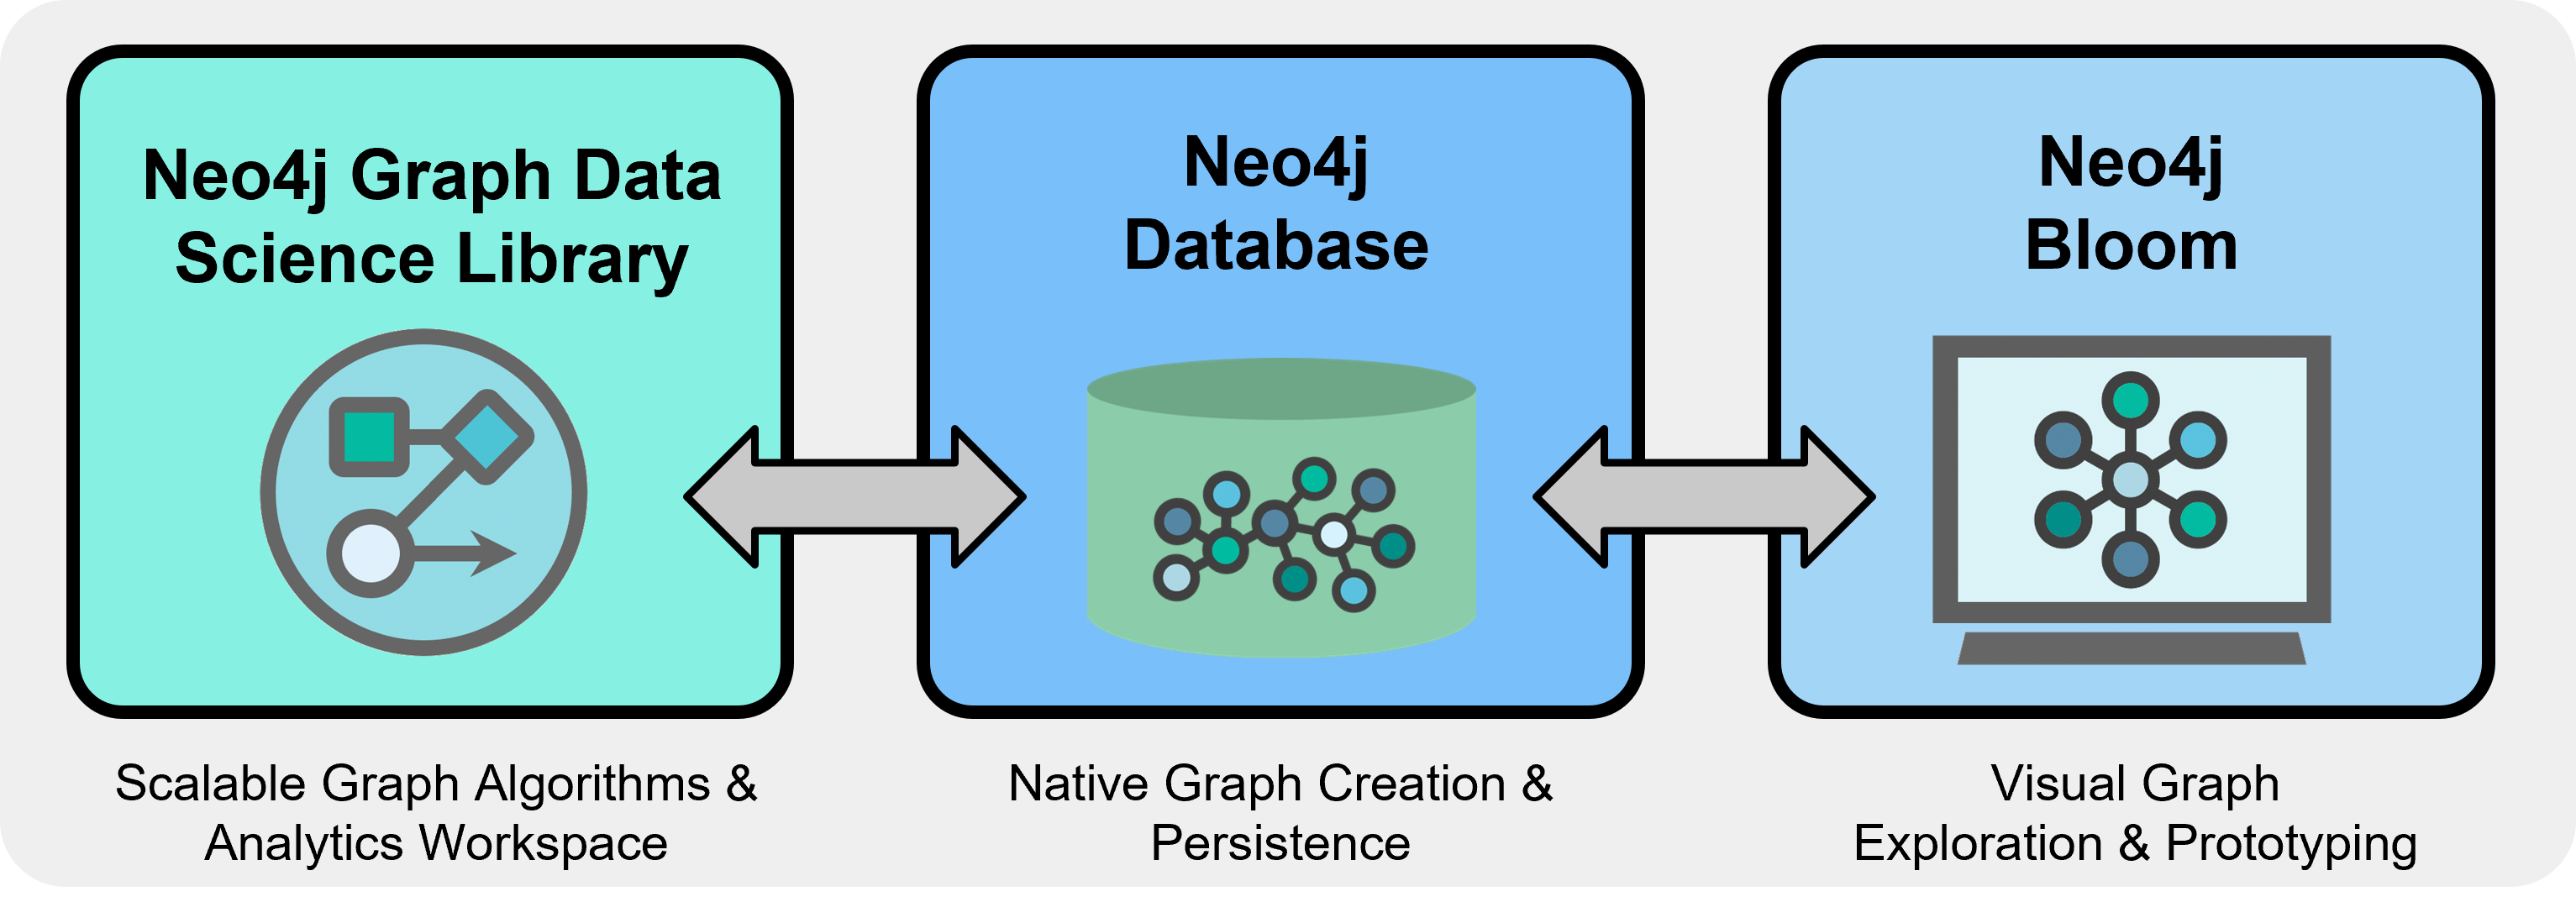
\includegraphics[width=\linewidth,keepaspectratio]{gds27}
\end{center}

\end{frame}

%%%%%%%%%%%%%%%%%%%%%%%%%%%%%%%%%%%%%%%%%%%%%%%%%%%%%%%%%%%%%%%%%%%%%%%%%%%%%%%%%%
\begin{frame}[fragile]\frametitle{Neo4j Graph Data Science Library}

\begin{center}
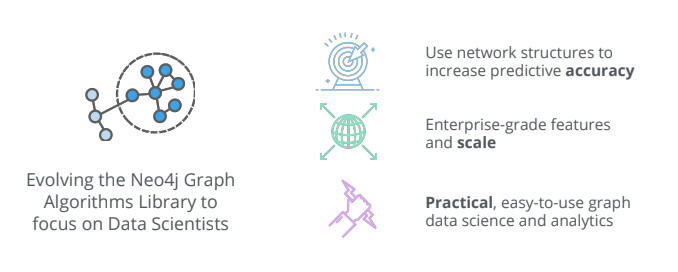
\includegraphics[width=\linewidth,keepaspectratio]{gds32}

{\tiny (Mark Needham - Intro to Graph Data Science with Neo4j)}

\end{center}

\end{frame}

%%%%%%%%%%%%%%%%%%%%%%%%%%%%%%%%%%%%%%%%%%%%%%%%%%%%%%%%%%%%%%%%%%%%%%%%%%%%%%%%%%
\begin{frame}[fragile]\frametitle{What’s available in GDS library?}

\begin{center}
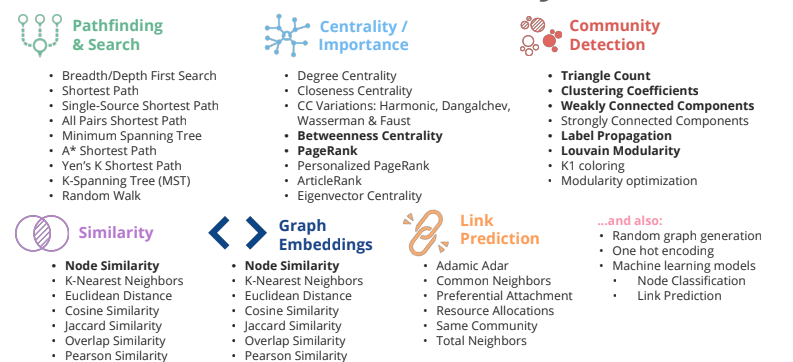
\includegraphics[width=\linewidth,keepaspectratio]{gds35}

{\tiny (Mark Needham - Intro to Graph Data Science with Neo4j)}

\end{center}

\end{frame}


%%%%%%%%%%%%%%%%%%%%%%%%%%%%%%%%%%%%%%%%%%%%%%%%%%%%%%%%%%%%%%%%%%%%%%%%%%%%%%%%%%
\begin{frame}[fragile]\frametitle{GDS syntax}

\begin{center}
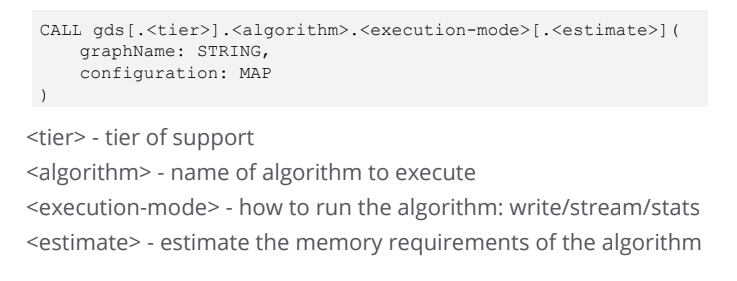
\includegraphics[width=\linewidth,keepaspectratio]{gds36}

{\tiny (Mark Needham - Intro to Graph Data Science with Neo4j)}

\end{center}

\end{frame}


%%%%%%%%%%%%%%%%%%%%%%%%%%%%%%%%%%%%%%%%%%%%%%%%%%%%%%%%%%%%%%%%%%%%%%%%%%%%%%%%%%
\begin{frame}[fragile]\frametitle{Tiers of Support}

\begin{center}
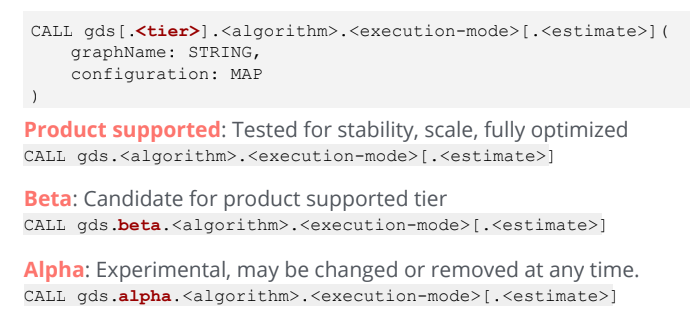
\includegraphics[width=\linewidth,keepaspectratio]{gds37}

{\tiny (Mark Needham - Intro to Graph Data Science with Neo4j)}

\end{center}

\end{frame}

%%%%%%%%%%%%%%%%%%%%%%%%%%%%%%%%%%%%%%%%%%%%%%%%%%%%%%%%%%%%%%%%%%%%%%%%%%%%%%%%%%
\begin{frame}[fragile]\frametitle{Where do I find the GDS library?}

\begin{center}
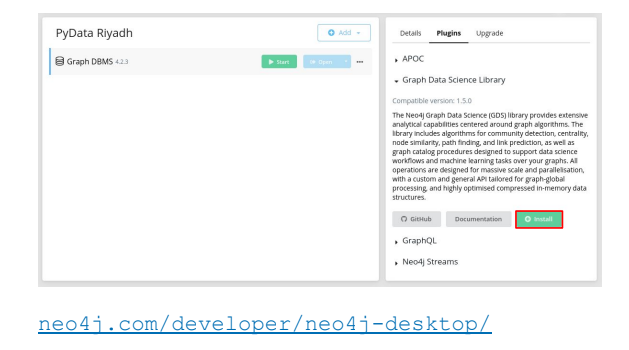
\includegraphics[width=\linewidth,keepaspectratio]{gds38}

{\tiny (Mark Needham - Intro to Graph Data Science with Neo4j)}

\end{center}

\end{frame}

%%%%%%%%%%%%%%%%%%%%%%%%%%%%%%%%%%%%%%%%%%%%%%%%%%%%%%%%%%%%%%%%%%%%%%%%%%%%%%%%%%
\begin{frame}[fragile]\frametitle{Where do I find the GDS library?}

\begin{itemize}
\item Download from: neo4j.com/download-center
\item Documentation: neo4j.com/docs/graph-data-science/1.5
\end{itemize}

\end{frame}

% %%%%%%%%%%%%%%%%%%%%%%%%%%%%%%%%%%%%%%%%%%%%%%%%%%%%%%%%%%%%%%%%%%%%%%%%%%%%%%%%%%
% \begin{frame}[fragile]\frametitle{Make Better Predictions}

% \begin{itemize}
% \item Answer intractable questions and increase predictive accuracy - with existing data
% \item First graph data science framework with enterprise features, scale, and support  
% \item Practical, easy-to-use graph data science and visual exploration
% \end{itemize}

% \end{frame}

%%%%%%%%%%%%%%%%%%%%%%%%%%%%%%%%%%%%%%%%%%%%%%%%%%%%%%%%%%%%%%%%%%%%%%%%%%%%%%%%%%
\begin{frame}[fragile]\frametitle{What Next?}

\begin{center}
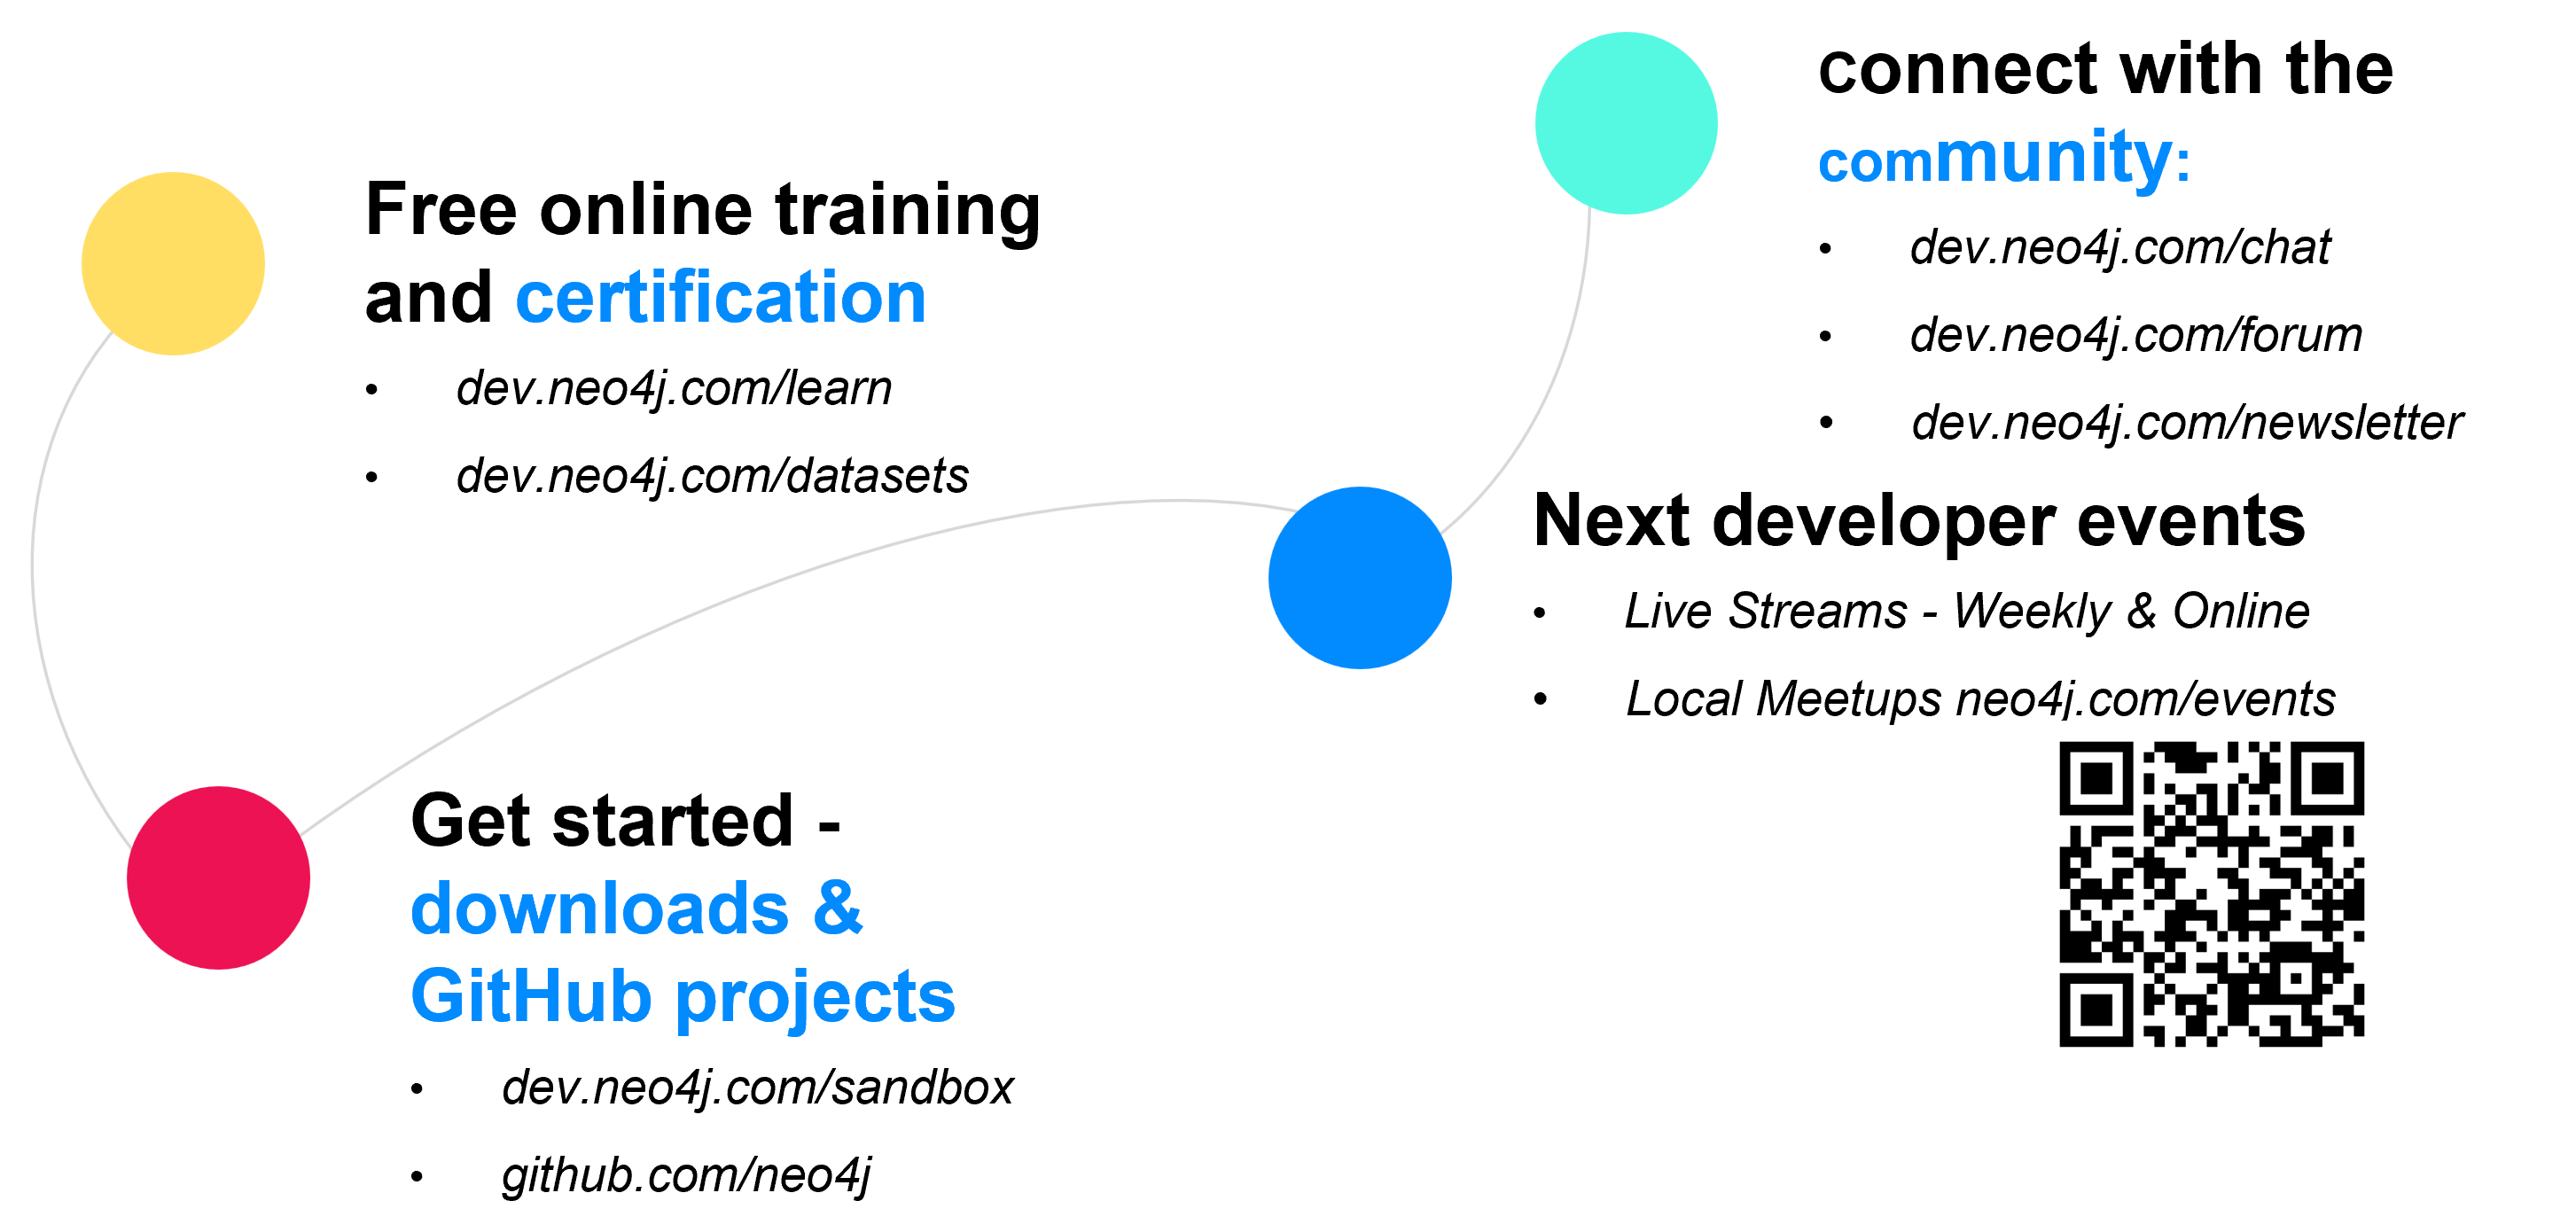
\includegraphics[width=\linewidth,keepaspectratio]{gds28}
\end{center}

\end{frame}

%%%%%%%%%%%%%%%%%%%%%%%%%%%%%%%%%%%%%%%%%%%%%%%%%%%%%%%%%%%%%%%%%%%%%%%%%%%%%%%%%%
\begin{frame}[fragile]\frametitle{Get Started \ldots}

\begin{itemize}
\item Download from: neo4j.com/download-center
\item Documentation: neo4j.com/docs/graph-data-science/1.5
\end{itemize}

\end{frame}
